% Arara build configuration:
% arara: pdflatex: {synctex: on, shell: true}
% arara: bibtex
% nomencl: {style: 'nomencl'}
% pdflatex: { synctex: on }
% pdflatex: { synctex: on }

%\includeonly{chap/legdesign}
\documentclass[listof=totoc,bibliography=totoc,11pt,twoside,BCOR=12mm,DIV=11]{scrbook}
\linespread{1.25}

\renewcommand*{\chapterheadstartvskip}{\vspace*{0cm}}

\renewcommand{\autodot}{}% Remove all end-of-counter dots
\addtokomafont{pagenumber}{\large\sffamily}

%\usepackage{showframe}  %to show typing area, header, footer, margins

\usepackage{microtype} %improve font spacing
\usepackage{parskip}

\usepackage[english]{babel}
\usepackage{amsmath}
\usepackage{amsfonts}
\usepackage{amssymb}
\usepackage[T1]{fontenc}
\usepackage{charter} %set font
%\setkomafont{disposition}{\bfseries}
\addtokomafont{chapter}{\Huge} %set font parameter
\addtokomafont{section}{\huge} %set font parameter
\addtokomafont{subsection}{\LARGE} %set font parameter
\addtokomafont{subsubsection}{\Large} %set font parameter

%\usepackage[headsepline,footsepline]{scrpage2}
%\pagestyle{scrheadings}
%\setheadsepline{3pt}

%\usepackage[round,mcite]{natbib} %bibliography

\usepackage[hidelinks]{hyperref} %hyperlinks in pdf
\usepackage{cleveref}
\crefname{subsection}{subsection}{subsections}

\usepackage{blindtext}  %to create a dummy document
\usepackage{lipsum} %content filler

\usepackage{minted}
\usemintedstyle{fruity}

\usepackage{float}
\usepackage{graphicx}
\DeclareGraphicsExtensions{.pdf,.png,.jpg,.eps} %images without extension
\usepackage{subfig} %use subfigure configurations
%\usepackage{caption}
%\usepackage{subcaption}
\usepackage{epstopdf} %include eps figures
\usepackage[final]{pdfpages} %includepdf
\usepackage[section]{placeins} %no [Htb], place within section
%\usepackage{showframe}

\usepackage{textcomp} %copyright symbols

%Nomenclature
\usepackage[intoc]{nomencl}
\makenomenclature

% customize dictum format:
\setkomafont{dictumtext}{\itshape\small}
\setkomafont{dictumauthor}{\normalfont}
\renewcommand*\dictumwidth{\linewidth}
\renewcommand*\dictumauthorformat[1]{--- #1}
\renewcommand*\dictumrule{}

\begin{document}

\frontmatter
\titlehead{
\begin{center}

\includegraphics[width = 0.35\textwidth]{images/uctround.png}
\end{center}
}
\subject{Faculty of Engineering and the Built Environment \\
Department of Electrical Engineering \\}
\title{{Hopping Control of a Single Leg Robot}}
\subtitle{Prepared for Dr. Amir Patel.
\linebreak
Submitted to the Department of Electrical Engineering\\at the University of Cape Town in partial
fulfilment\\ of the academic requirements\\for a Bachelor of Science (Eng.) degree in Mechatronics.
}
\author{Benjamin Scholtz}
%\date{date}
\publishers{\textbf{Keywords:} robotics, virtual model, compliance control, force control, mechatronics}
\dedication{To all the people that helped me jump!\\ \medskip \includegraphics[width = 0.4\textwidth]{images/leg-mount.png}}
\maketitle
\chapter{Declaration}
\begin{enumerate}
\item I know that plagiarism is wrong. Plagiarism is to use another's work and pretend that it
is one's own.
\item I have used the IEEE convention for citation and referencing. Each contribution to, and
quotation in, this final year project report from the work(s) of other people, has been attributed and has been cited and referenced.
\item This final year project report is my own work.
\item I have not allowed, and will not allow, anyone to copy my work with the intention of passing it off as their own work or part thereof.
\end{enumerate}

\bigskip

\noindent
Name: Benjamin Scholtz \\
Signature: \underline{\hspace{3cm}} \\
Date: \today \\
\chapter{Abstract}

A vertically constrained direct drive robotic leg platform was modelled, simulated, designed, built, and tested in order to better understand rapid acceleration control. The research was performed to investigate the following questions: \textbf{Is a virtual model a suitable replacement for accurate dynamic modelling in complex robotic topologies? Can high fidelity force control be effectively implemented without using force feedback? Is a virtual compliance control system effective in handling high speed impacts and executing rapid acceleration manoeuvres?} The dynamic model of the robot is complex, instead a virtual model uses simulations of components placed on the body of the robot to generate the desired end effector force response. The end effector was virtually modelled in the polar coordinate system as a radial and torsional series spring-damper. The desired virtual model motor torques were generated using the Jacobian kinematic mapping. Proprioceptive force control was possible due to the transparent coupling between the direct drive actuator and end effector. An iterative hardware and software design process was used to enable effective robotic testing - both an embedded communication and control system, and a GUI, were developed for the platform. Experiments were performed in virtual model spring-damping, impact absorption, trajectory tracking, force control, and current control. Jump tests were performed investigating robustness, repeatability, and rapid acceleration control. Force control and virtual model fidelity were verified by critically analysing both theoretical simulated responses and practical data. The robot generated an energy of $3.9\ J/kg$ with a maximum hopping height of $0.4\ m$, comparing well to the current state of the art. Robust hopping control was achieved with an $8.57\%$ mean time shift and a negligible mean peak force deviation over 7 consecutive jumps. A robust robotic platform was successfully developed that enabled high fidelity force control using a virtual compliance model. The research contributed a platform and control framework that can be effectively used in future rapid acceleration research in the UCT Mechatronics Lab.


\chapter{Acknowledgements}
Amir Patel
Callen Fisher
Craig Burden
Gareth Callanan
Roberto Aldera

Ben Bingham
Luke Bell

Justin Pead
Brendan Daniels
\chapter{Terms of Reference}

\section*{Description}

\begin{figure}[H]
\centering
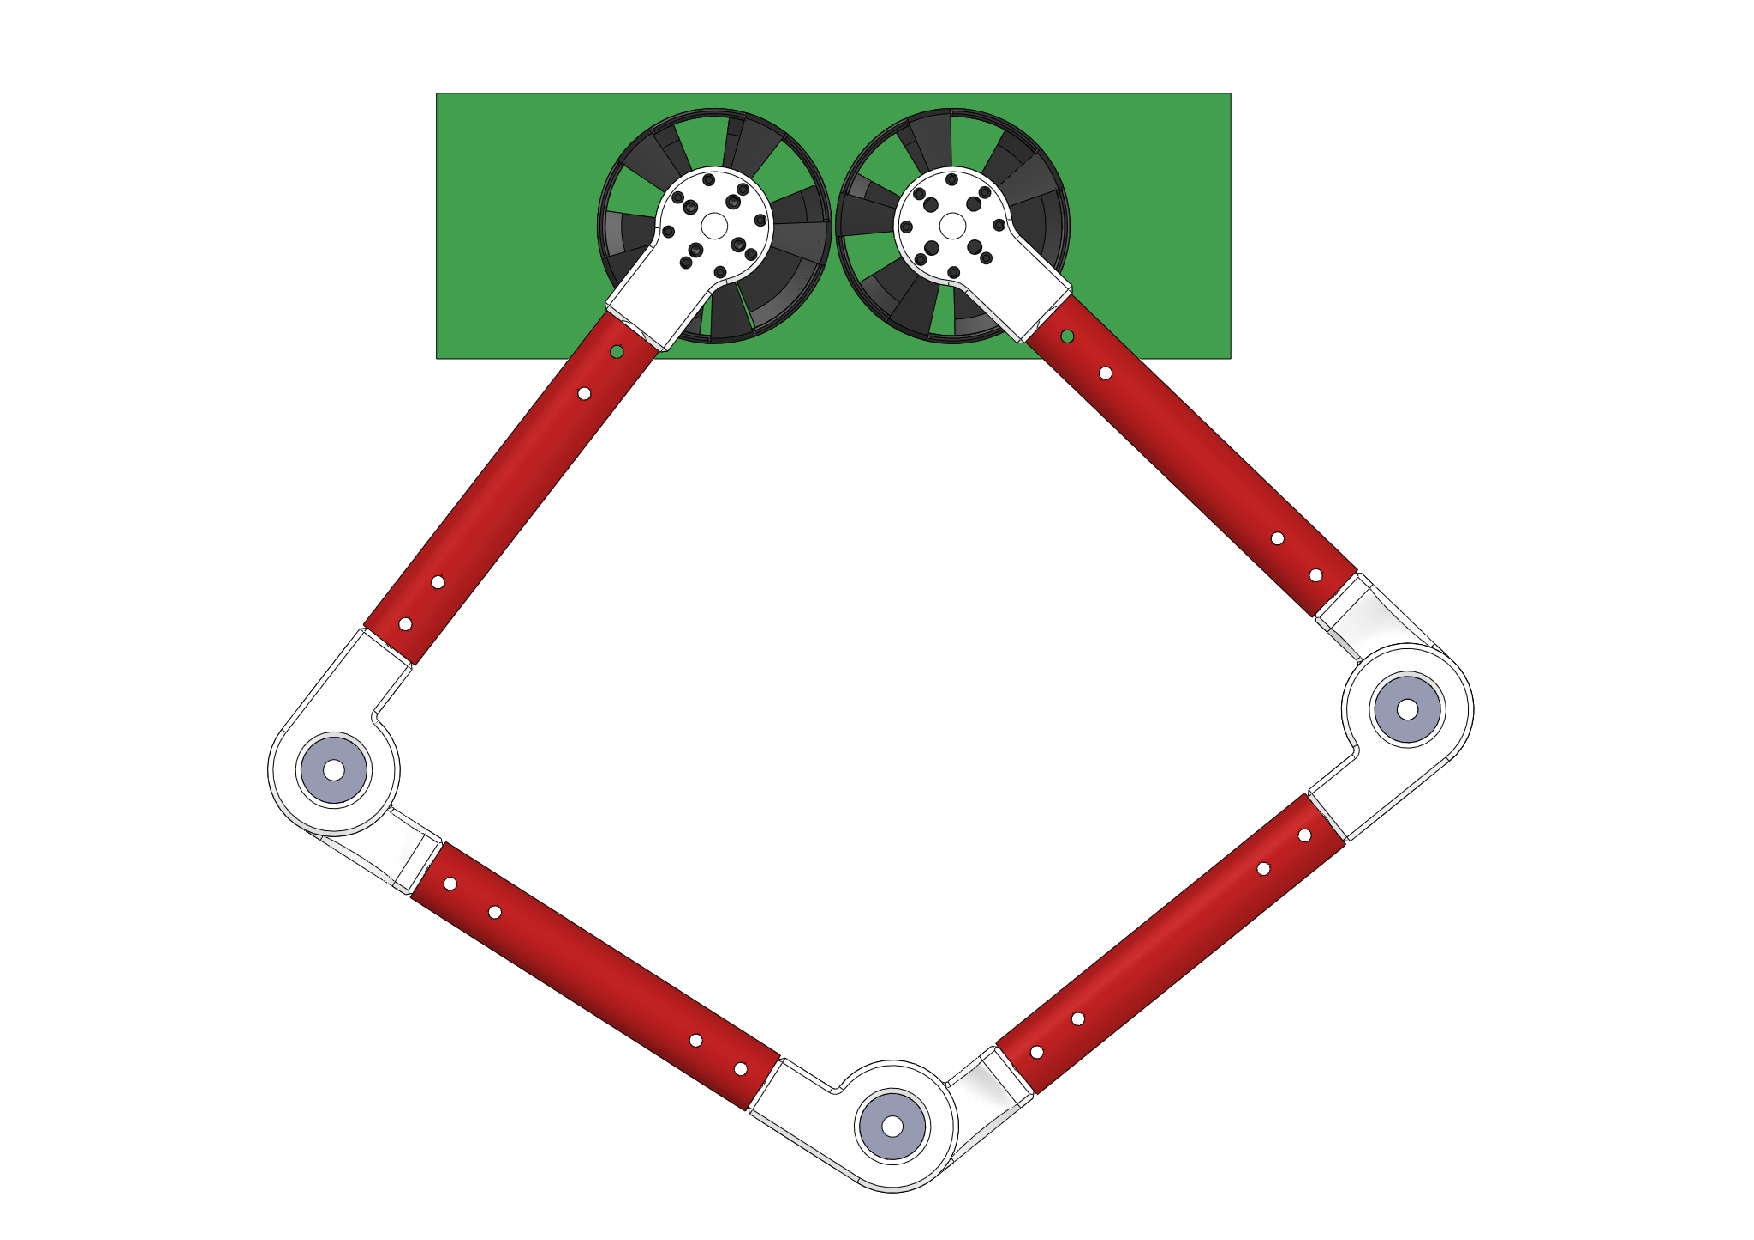
\includegraphics[width=0.5\textwidth,trim={0cm 0cm 0cm 0cm},clip]{images/mechanical/legsV1.pdf}
\caption{Version 1 of Baleka leg platform (Ben Bingham, 2016).}
\label{fig:legV1}
\end{figure}

The Mechatronics Lab has recently developed a single leg direct drive robot,
Baleka, to investigate modelling and control of rapid accelerations.
This project will involve the design of a control system to perform stable
hopping with the robot. Various controller algorithms will be investigated and
compared (eg. PID, MPC, etc.). The project will also involve developing a test
rig for the robot.

\section*{Deliverables}

\begin{itemize}
\item Mathematical model of the hopping robot must be developed in
Simulink/Matlab
\item Hopping controller design
\item Mechanical design of the test rig
\item Experimental testing of the robot
\end{itemize}

\section*{Skills/Requirements}

\begin{itemize}
\item Mathematical Modelling 
\item Mechatronics Design
\item Control Systems
\item Embedded Systems
\item Strong Practical and Mathematical skills required
\end{itemize}

\section*{ELO3: Engineering Design}

\textit{Perform creative, procedural and non-procedural design and synthesis of components, systems, engineering works, products or processes.}

The student is expected to design:

\begin{itemize}
\item Robot feedback control system
\item Rig for testing of hopping motion
\end{itemize}

\section*{Area of Research}

\begin{itemize}
\item Bio-inspired robotics
\item Control systems
\end{itemize}

\section*{Extra Information}

\url{http://ieeexplore.ieee.org/xpls/abs_all.jsp?arnumber=5648972}
\url{http://kodlab.seas.upenn.edu/uploads/Avik/compositionTR_sc.pdf}


\textsf{\tableofcontents}

\listoffigures
\listoftables
\renewcommand\listoflistingscaption{List of Source Codes}
\listoflistings

%\printnomenclature

\mainmatter

\setchapterpreamble[uc][.75\textwidth]{%
\dictum[Lewis Carroll, \textit{Alice in Wonderland}]{%
``Begin at the beginning,'' the King said, gravely, ``and go on till you
come to an end; then stop.''}\vskip1em}
\chapter{Introduction}
\label{chap:intro}

With a hop, skip, and a jump -- the journey begins!

\section{Background}
\section{Objectives of the Study}
\subsection{Problems to be Investigated}
\subsection{Research Questions}
\subsection{Purpose of the Study}
\section{Scope and Limitations}
\section{Plan of Development}
\chapter{Literature Review}
\section{Legged Locomotion in Nature}
\section{Raibert Control}
\cite{Raibert1977}
\cite{Raibert1984}
\cite{Raibert1989}

\subsection{Dynamic Stability vs Static Stability}
\subsection{Phases of Motion}
\subsection{Leg Stance Control}
\section{Force Control}

\setchapterpreamble[uc][.75\textwidth]{%
\dictum[Sherlock Holmes in Arthur Conan Doyle, \textit{The Crooked Man}]{%
``You know my methods, Watson.''}\vskip1em}
\chapter{Project Plan and Methodology}
\lipsum
\chapter{Kinematics}

The 5-bar linkage design of the leg was first designed constructed in the study \cite{Duperret}. The geometry of the leg is fairly complex and the derivation of the kinematic equations equally so. J.M. Duperret and D.E. Koditschek derived the kinematic equations \cref{eq:forward-kinematics, eq:reverse-kinematics} in the study \cite{Duperret}. 

In this study the assumption was made that the distance $d$, as seen in \cref{fig:Geometric view of leg}, is zero. This simplifies the derivation of forward and reverse kinematic equations of the leg design by making the leg a 4-bar linkage. These kinematic equations are more easily calculated on board a microcontroller\cite{Duperret}, leaving more processing power for other control tasks if needed. 

The ease of calculation makes the loss in accuracy acceptable - in practise the simplified kinematic equations worked well with an insignificant calculation time made possible by the STM32F4's on-board floating point unit.

\begin{equation} \label{eq:forward-kinematics}
f(\phi_1, \phi_2) = \left(\begin{array}{c} \sqrt{{\mathrm{l_2}}^2 - {\mathrm{l_1}}^2\, {\sin\!\left(\frac{\mathrm{\phi_1}}{2} + \frac{\mathrm{\phi_2}}{2}\right)}^2} - \mathrm{l_1}\, \cos\!\left(\frac{\mathrm{\phi_1}}{2} + \frac{\mathrm{\phi_2}}{2}\right)\\
\frac{\mathrm{\phi_1}}{2} - \frac{\mathrm{\phi_2}}{2} \end{array}\right)
\end{equation}

\begin{equation} \label{eq:reverse-kinematics}
g(r, \theta) = \left(\begin{array}{c} \pi - acos(\frac{r^2 + l_1^2 - l_2^2}{2rl_1}) + \theta \\
\pi - acos(\frac{r^2 + l_1^2 - l_2^2}{2rl_1}) - \theta  \end{array}\right)
\end{equation}

\section{The Jacobian}
The Jacobian is formed by taking partial derivatives of the forward kinematic equation \cref{eq:forward-kinematics} as shown in \cref{eq:jacobian}. 

It is used as a mapping from the joint angles $\phi_1$ and $\phi_1$ to the end effector generalized coordinates $r$ and $\theta$. The Jacobian can be applied in robotic kinematic control to determine joint velocities and forces to achieve a desired force or velocity at the end effector, in this case the leg foot.

Taking the Jacobian of the kinematic mapping $f(\phi_1, \phi_2)$ the foot force vector, F, can be transformed to the motor torque commands, $\tau$:
\begin{equation} \label{eq:jacobian}
J = \left[ \frac{\partial \textbf{f}}{\partial \textbf{X}} \right] 
\end{equation}
where \textbf{X} = [r $\theta$].

\subsection{Velocity Mapping}

Velocity mapping from motor rotational velocity to polar velocity.
\begin{equation}
v(\dot{r}, \dot{\theta}) = J w(\dot{\phi_1}, \dot{\phi_2})
\end{equation}


\chapter{Dynamic Modelling}
\section{System Modelling}

\begin{figure}
\centering
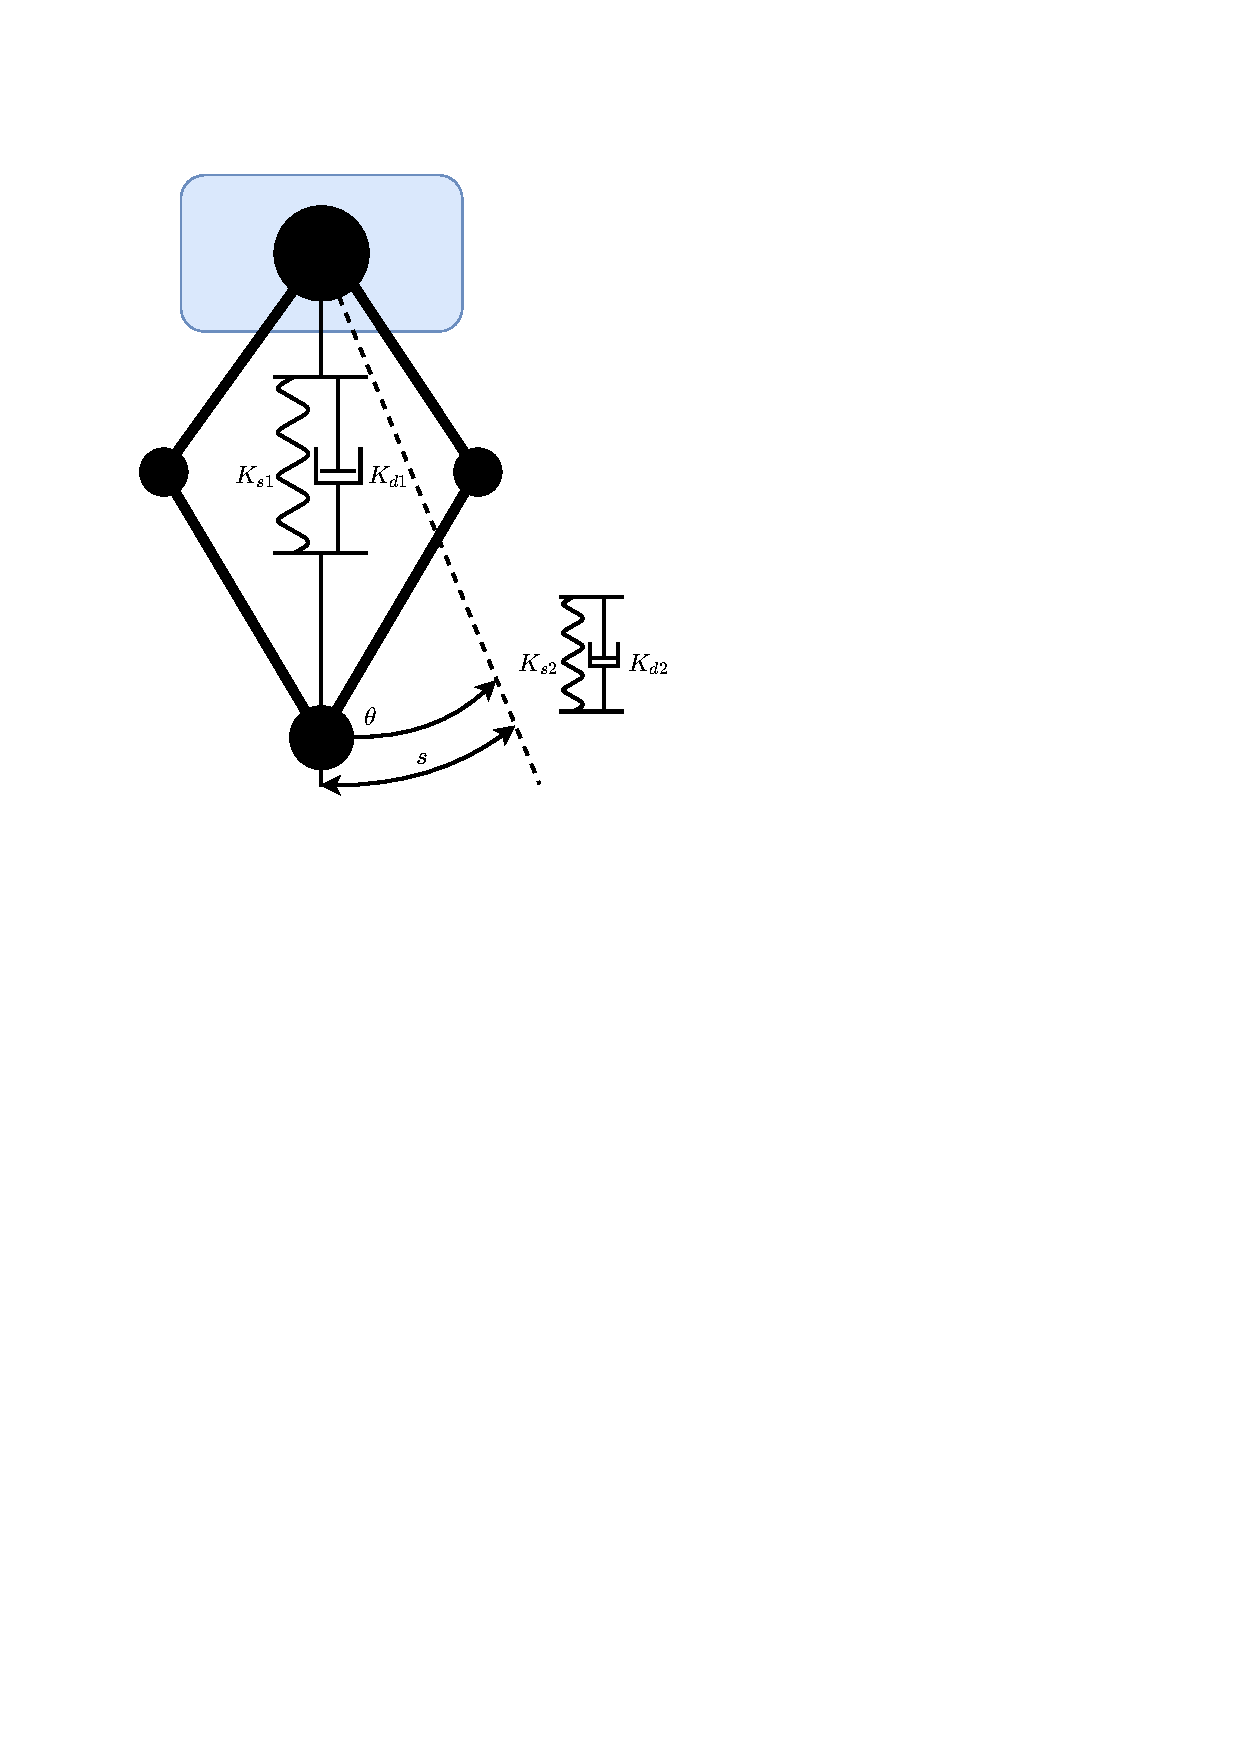
\includegraphics[clip, trim=2cm 15cm 9cm 2cm, page = 1, width=0.8\textwidth]{images/geometry/leg-spring-damper} 
\caption{Leg spring-damper virtual model.}
\label{fig:Leg spring-damper virtual model}
\end{figure}

\subsection{SLIP Model}
\section{Virtual Compliance Model}
\chapter{Hardware Design}

\section{Original Leg Design}
\label{sec:Original Leg Design}

\subsection{Leg Hip}
The original leg `hip' was designed by Ben Bingham in 2016 in completion of his undergraduate vacation work as seen in \cref{fig:original-hip}.

The `hip' was constructed of 6 mm perspex sheet in a box design with metal L connectors to join the sheets securely. The design of the `hip' allowed the motor drivers as well as the microcontroller to be mounted on the body, with space provided for an extra leg for future two-legged movement. 

\begin{figure}
\centering
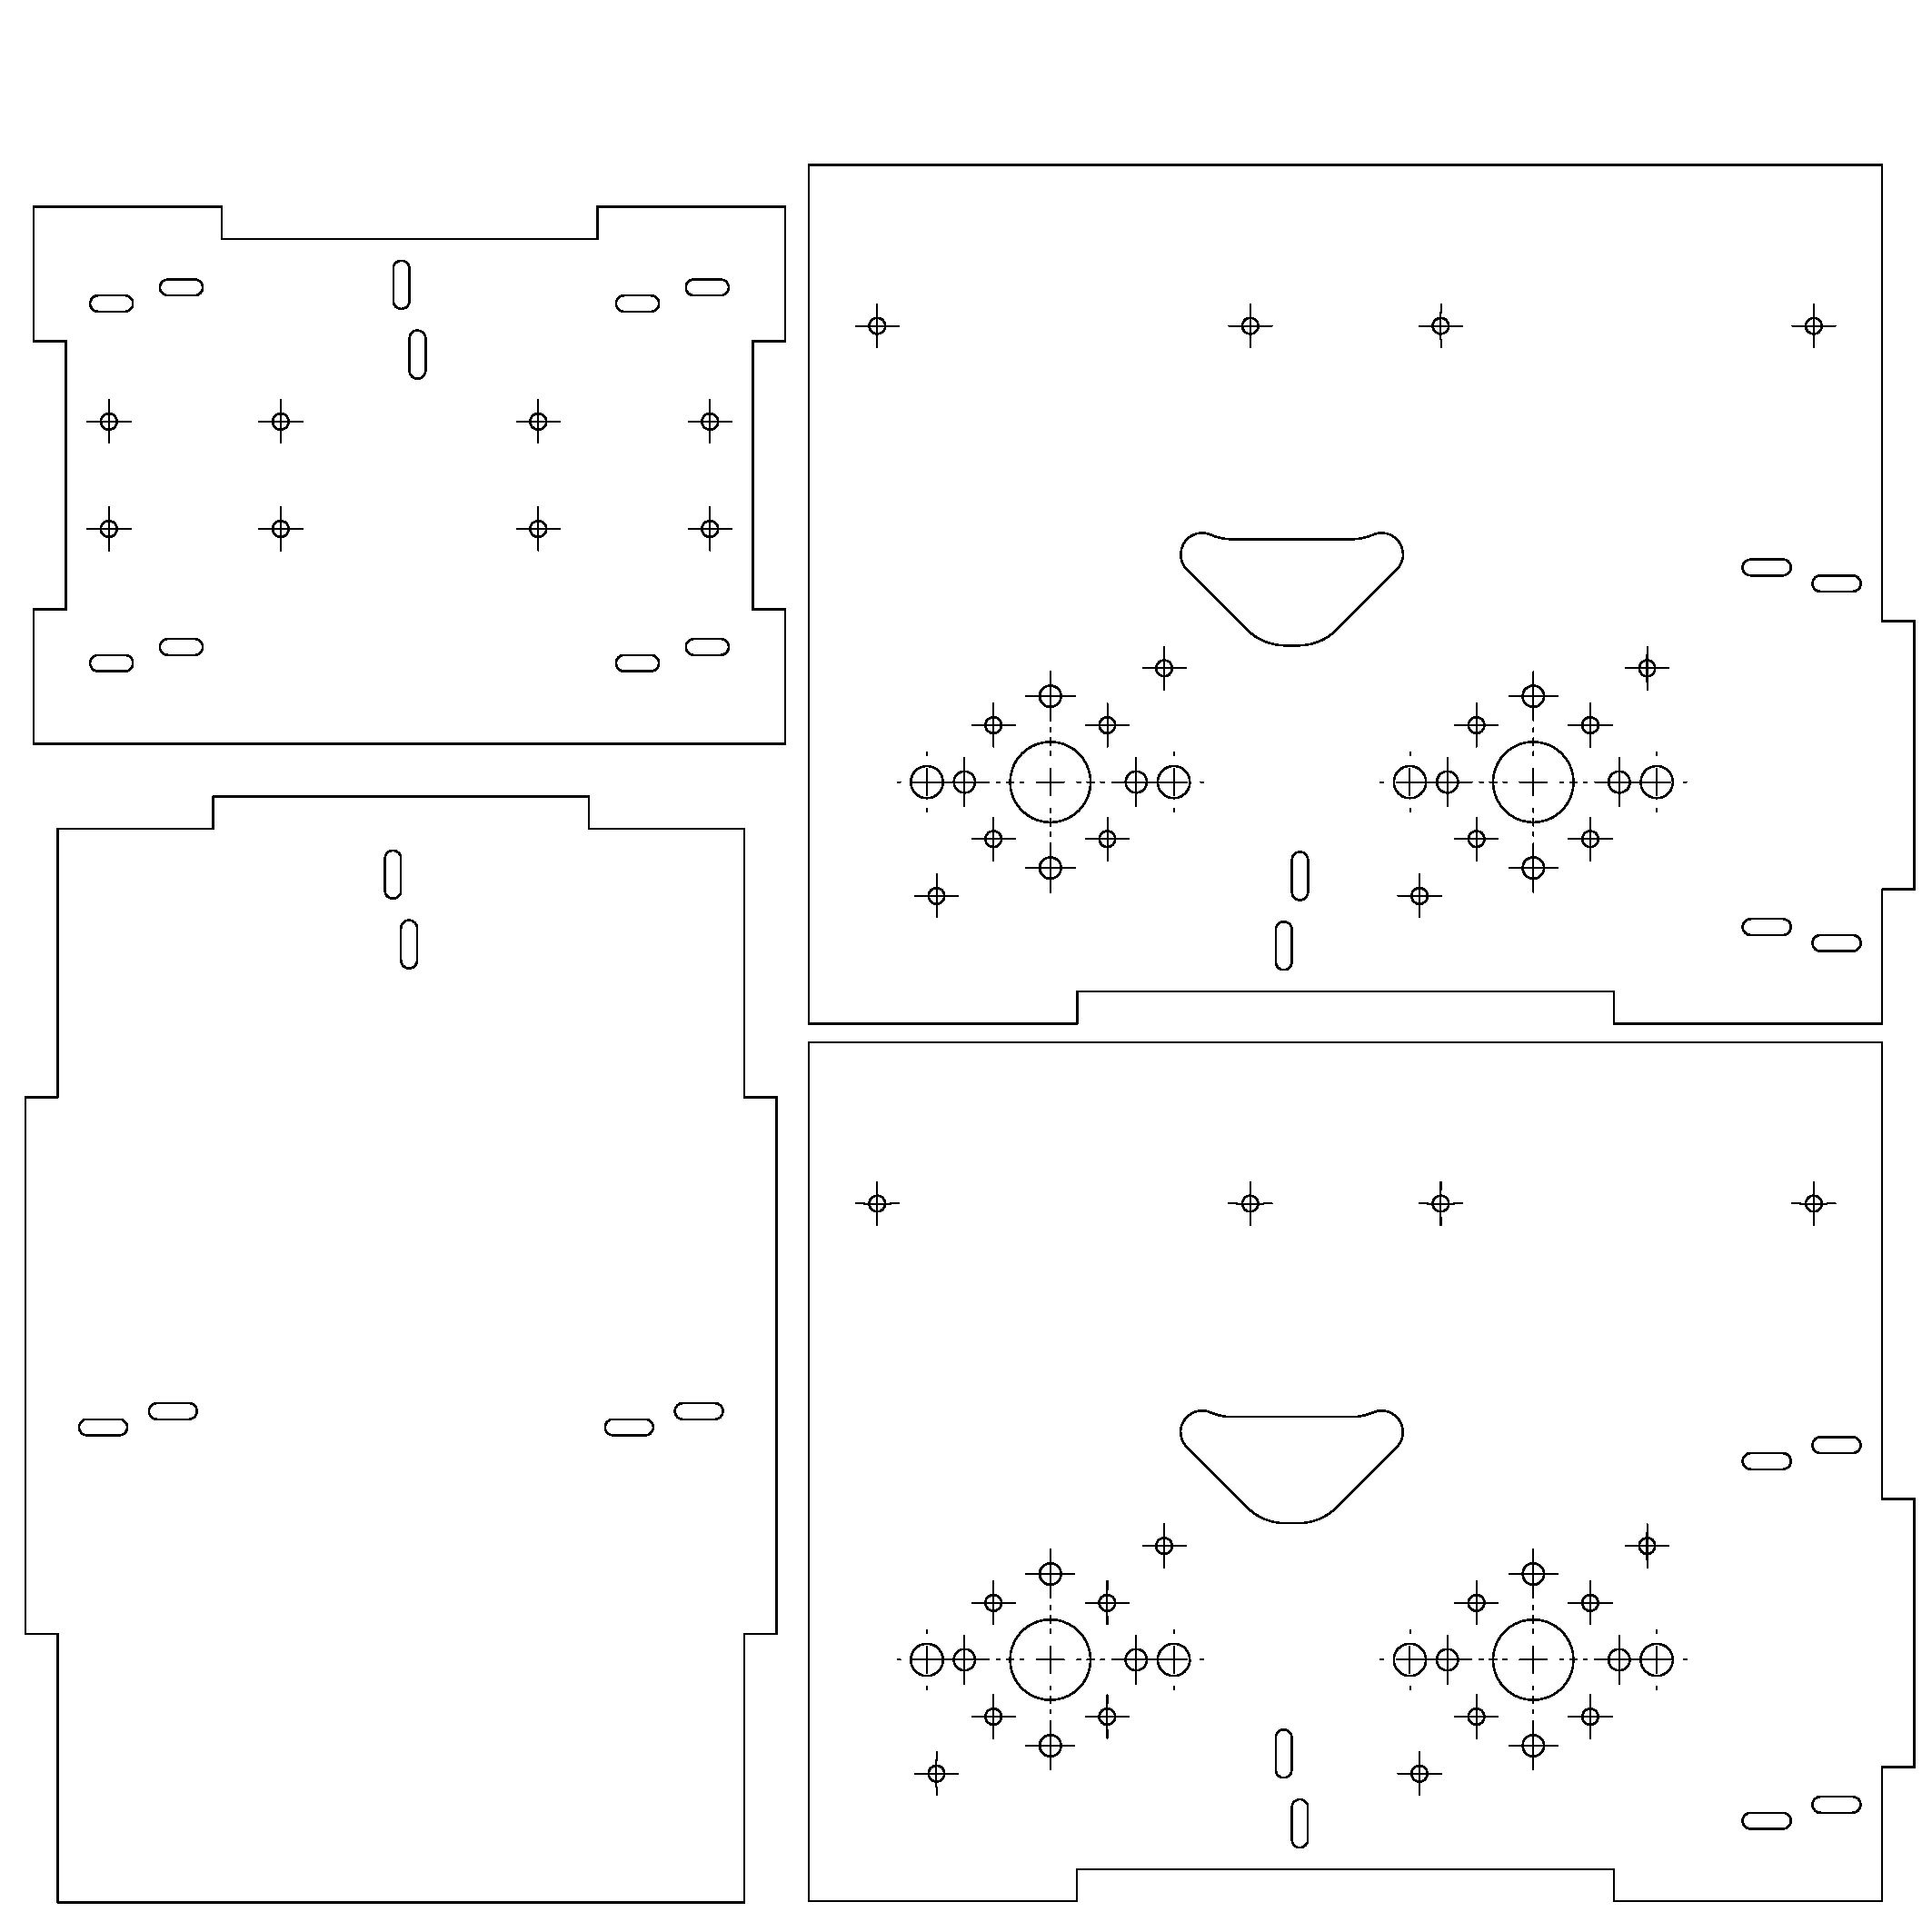
\includegraphics[clip, trim =0cm 0cm 0cm 0cm, page =1, width=0.4\textwidth]{images/mechanical/hip-6mm-360x360}
\caption{Original 'hip' design by Ben Bingham, 2016.}
\label{fig:original-hip}
\end{figure}

\subsection{Leg Guide}
The guiding system consisted of two parallel steel rods with ball bearings mounted on the `hip'. The ball bearings were mounted using a 3D printed holder, with one for each circular  bearing. 

\subsection{Limitations}

The leg mounting plate went through three design iterations after the original `hip' design before the final design was created, as seen in \cref{fig:CAD mounting plate final design}.

The original `hip' design had the following mechanical design flaws:

\begin{enumerate}
\item The 6 mm perspex box construction with on-board microncontroller and motor drivers was too heavy for efficient jumping action when compared to similar designs like \cite{Duperret} (1.3 kg), \cite{Kalouche2016} (2.5 kg), \cite{Wang2012} (4.2 kg) where there is a high leg torque to mass ratio.
\item The ball bearings are particularly heavy.
\item The mounting of the leg guide places a significant torque in all three cartesian coordinates being off-center from the center of mass.
\item The design of the leg guide requires the two steel rods to be perfectly parallel to remove resistance to movement, which is difficult to achieve practically.
\end{enumerate}

These problems were accounted for by replacing the original `hip' with a rigid aluminium mounting plate with off-board microcontroller and motor drivers. The leg guide consisting of parallel steel rods and ball bearings was replaced with a linear guide as seen in \cref{fig:drylin-linear-guide}.  

\begin{figure}
\centering
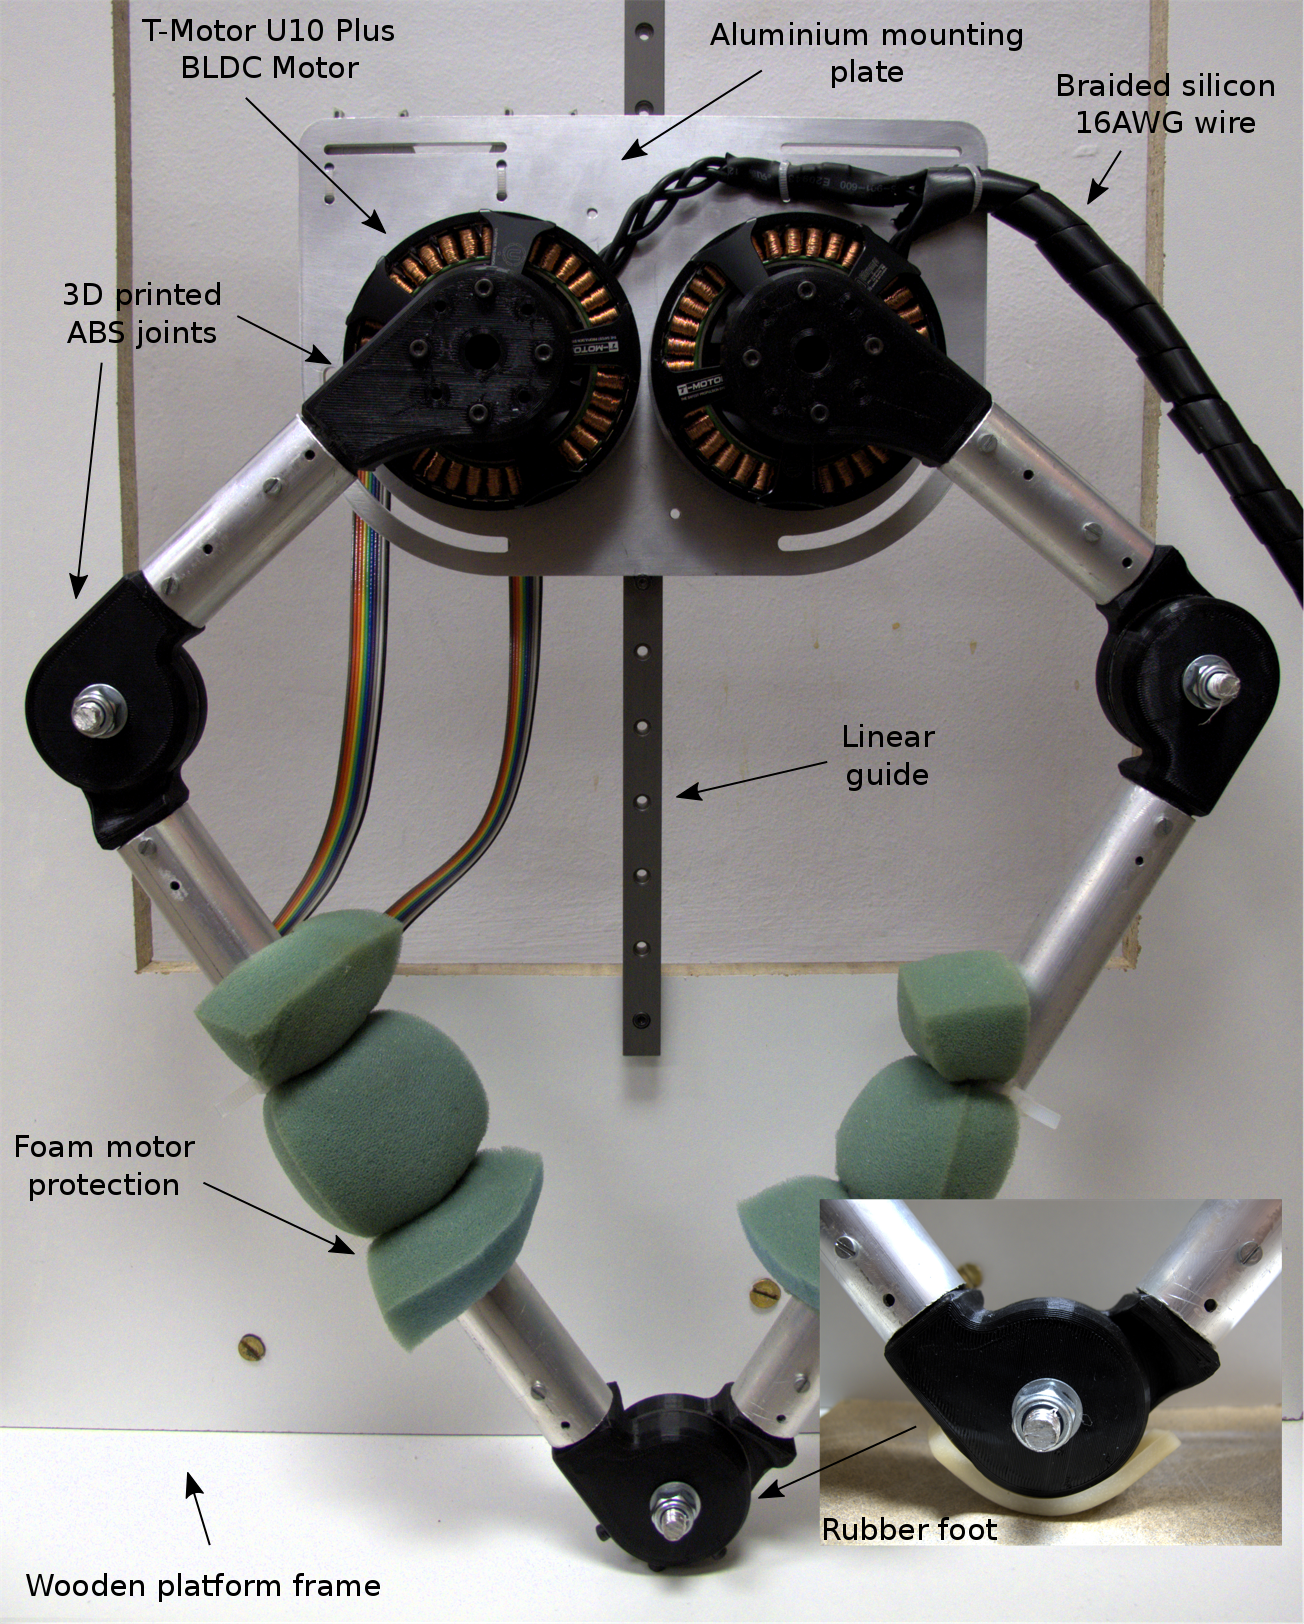
\includegraphics[width=0.8\textwidth]{images/mechanical/leg-mount-annotated} 
\caption{Final leg design mounted to platform and linear guide: front.}
\label{fig:Final leg design - front}
\end{figure}

\begin{figure}
\centering
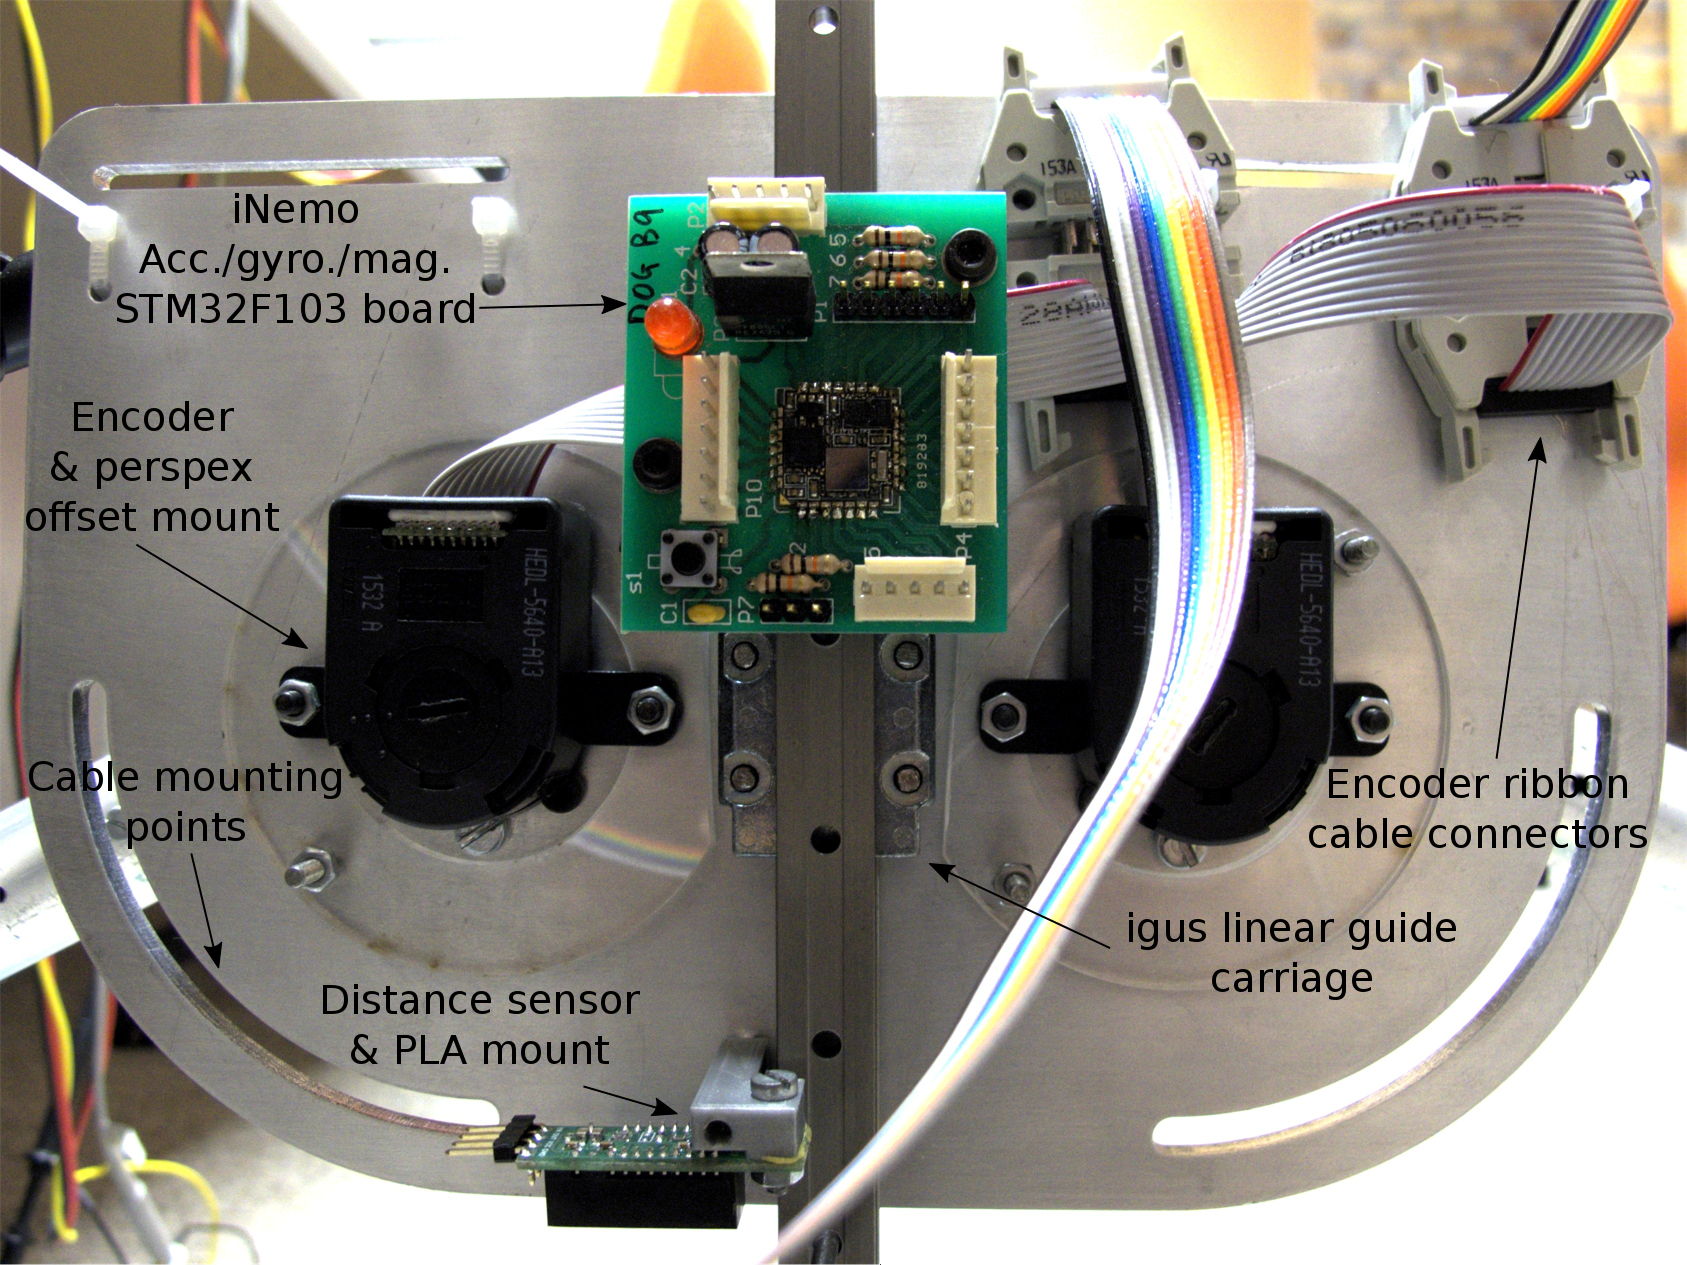
\includegraphics[width=0.8\textwidth]{images/mechanical/encoder-mount-annotated} 
\caption{Final leg design mounted to platform and linear guide: back.}
\label{fig:Final leg design - back}
\end{figure}

\section{Mechanics and Construction}

\subsection{Aluminium Mounting Plate Design}
\label{sec:Alumnium Mounting Plate Design}

The original mounting box described in \cref{sec:Original Leg Design} was replaced with a single mounting plate. 

In order to reduce the weight of the platform and to prevent damage to components during jump tests, the motor drivers and microcontroller were mounted off-board on a separate mounting plate - the final design of which can be seen in \cref{fig:Motor driver interface mounting plate}.

The plate that the motors and encoders mount to went through several iterations before the final design was used. A few major factors were considered in the design process, both for the motor mount and motor driver mount:
\begin{enumerate}
\item Perspex material was too flexible, especially considering the close tolerances of the motor mounts - aluminium was used instead of perspex as a more rigid material.
\item The motors when used in a high torque relatively static environment reach temperatures of close to $100^oC$ - this heat was noticeably better dissipated by aluminium.
\item The motor drivers perform better and are less likely to thermally cut-out if mounted on aluminium.
\item The center of mass of the robotic leg body was calculated and the linear guide mount was placed as close as possible to this point. This ensured as little torque as possible was placed on the linear guide which would lead to frictional losses and ware.
\item The iNemo accelerometer, gyroscope, magnetometer combination was placed as close as possible to the center of mass to ensure proper readings were achieved which accurately represented the robot dynamics.
\item Excess weight was cut wherever possible, most noticeably so above the motor mounting points.
\end{enumerate}


\begin{figure}
\centering
\subfloat[][CAD mounting plate V1.]{
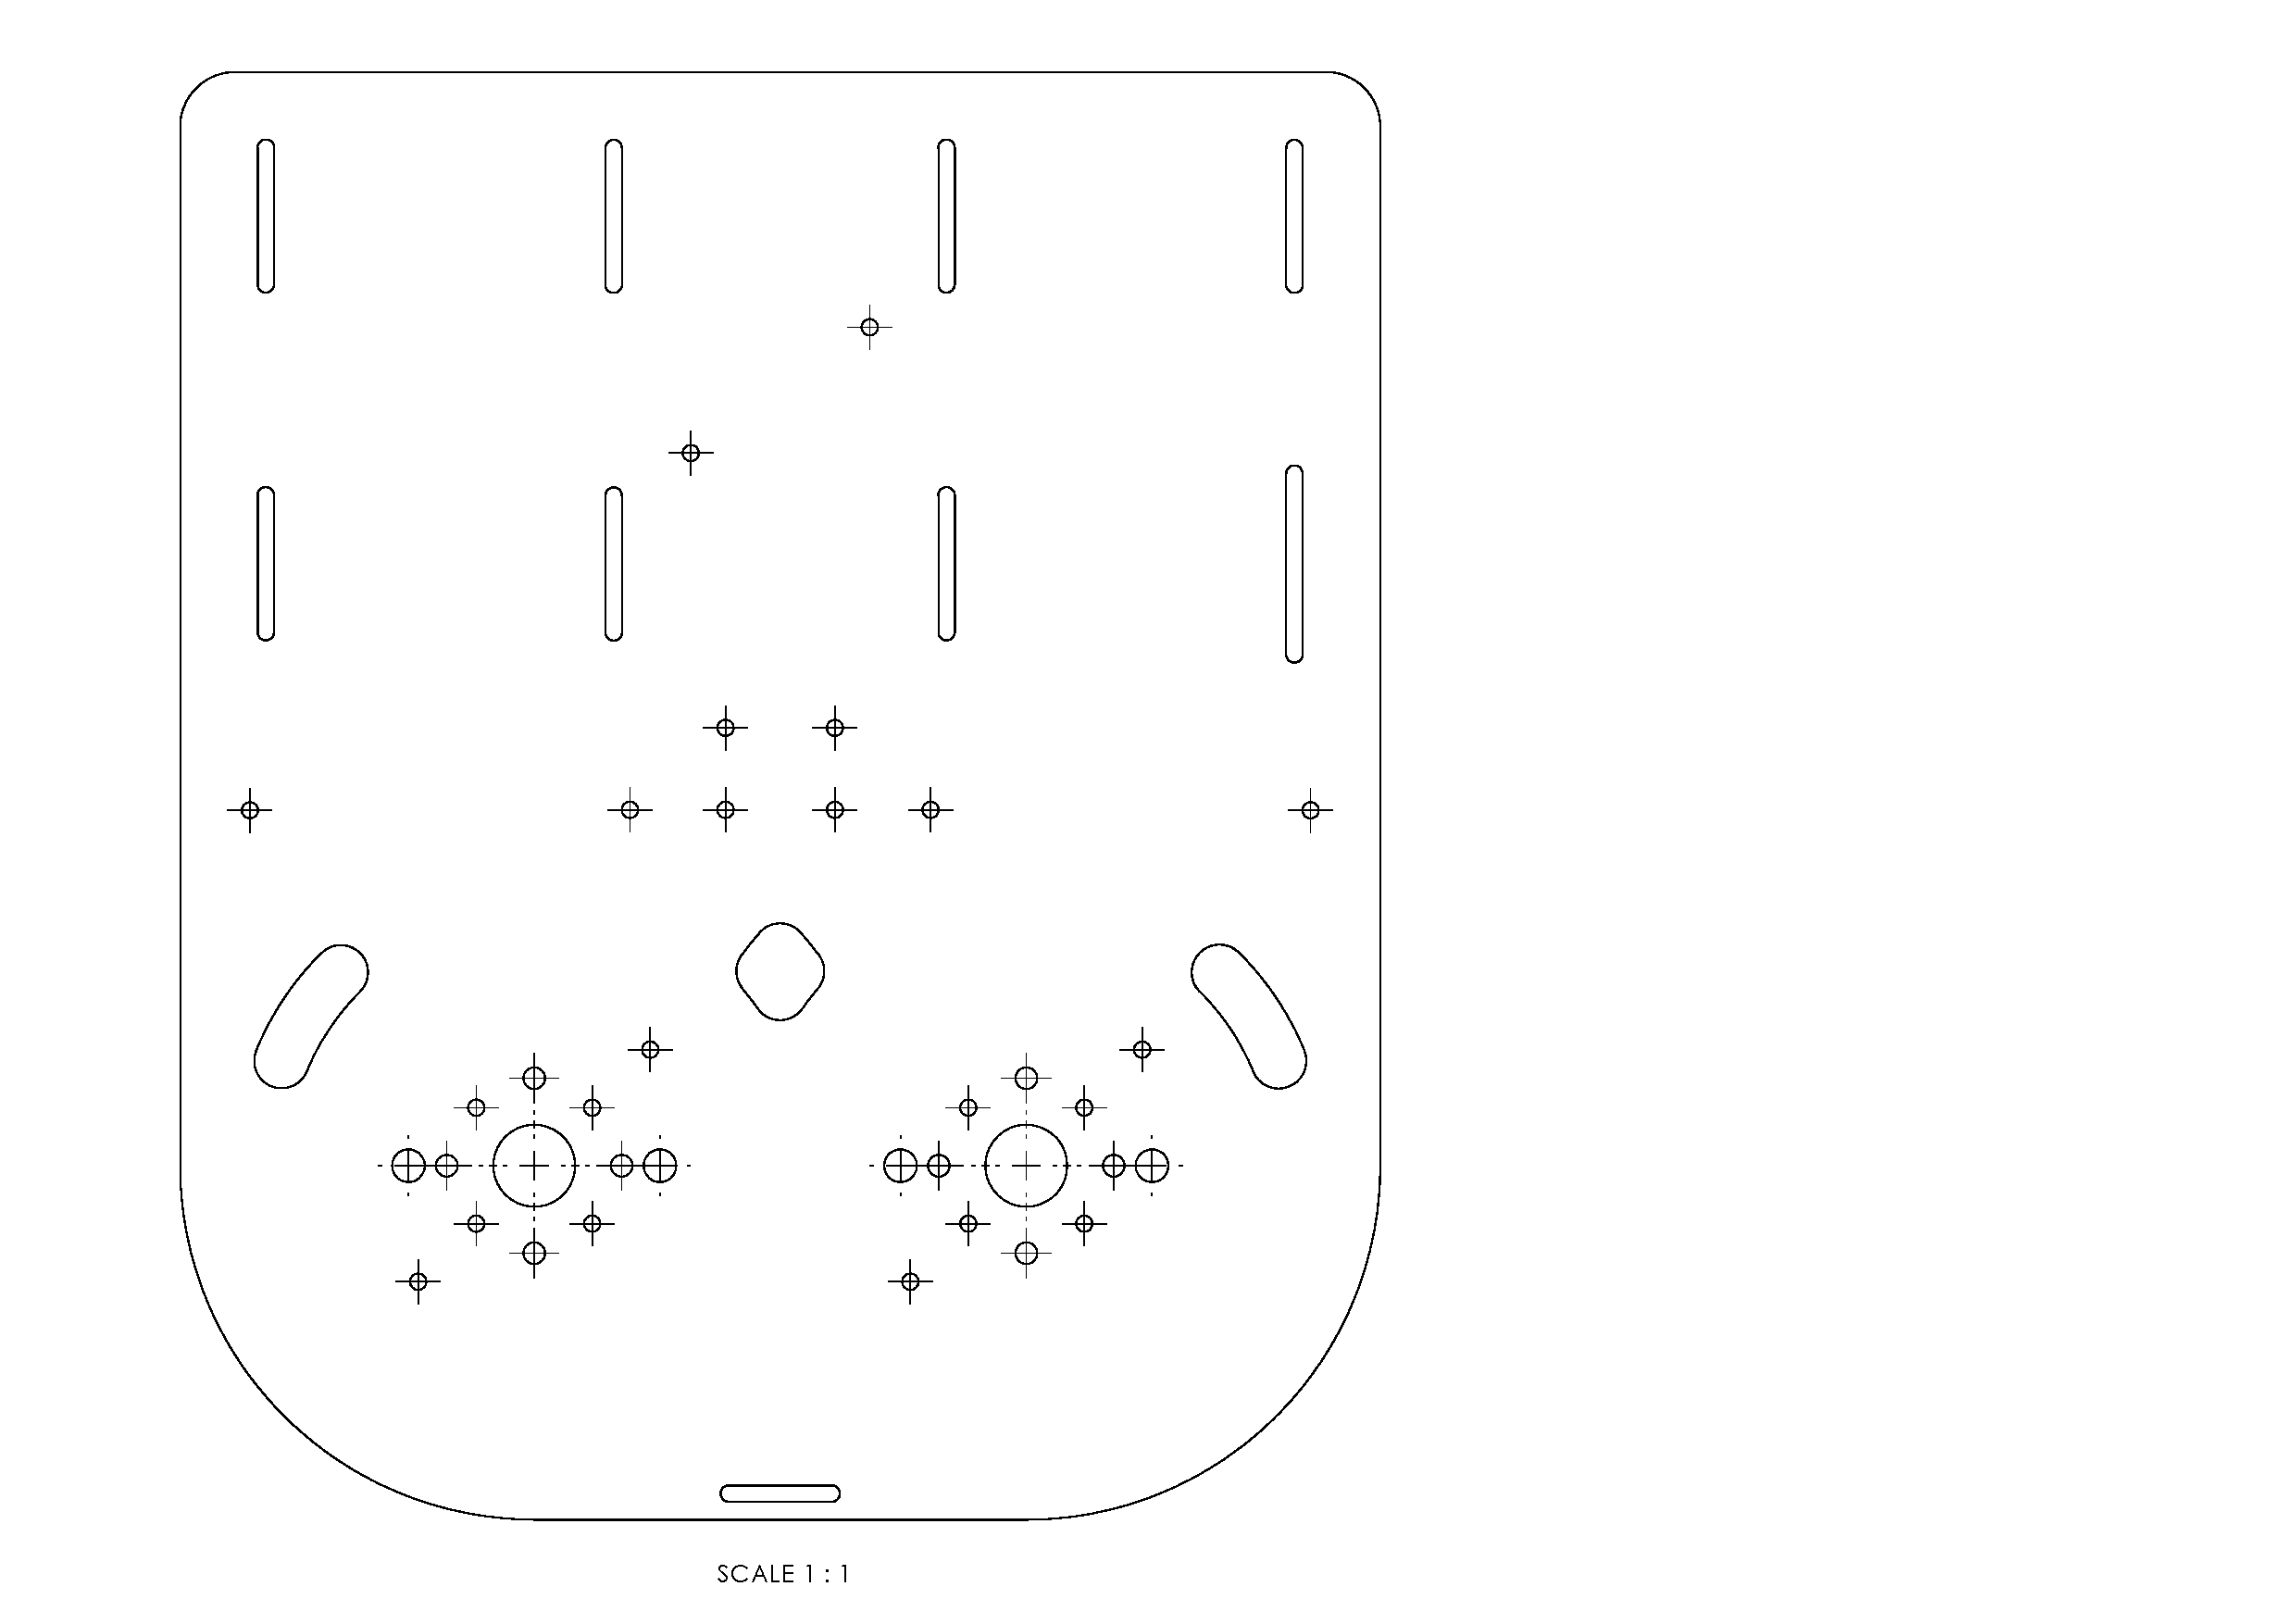
\includegraphics[clip, trim=2cm 0cm 16cm 1cm, page = 1, width=0.3\textwidth]{images/mechanical/laser-test-print-V1} 
\label{fig:CAD mounting plate V1}
}
\subfloat[][CAD mounting plate V3.1.3.]{
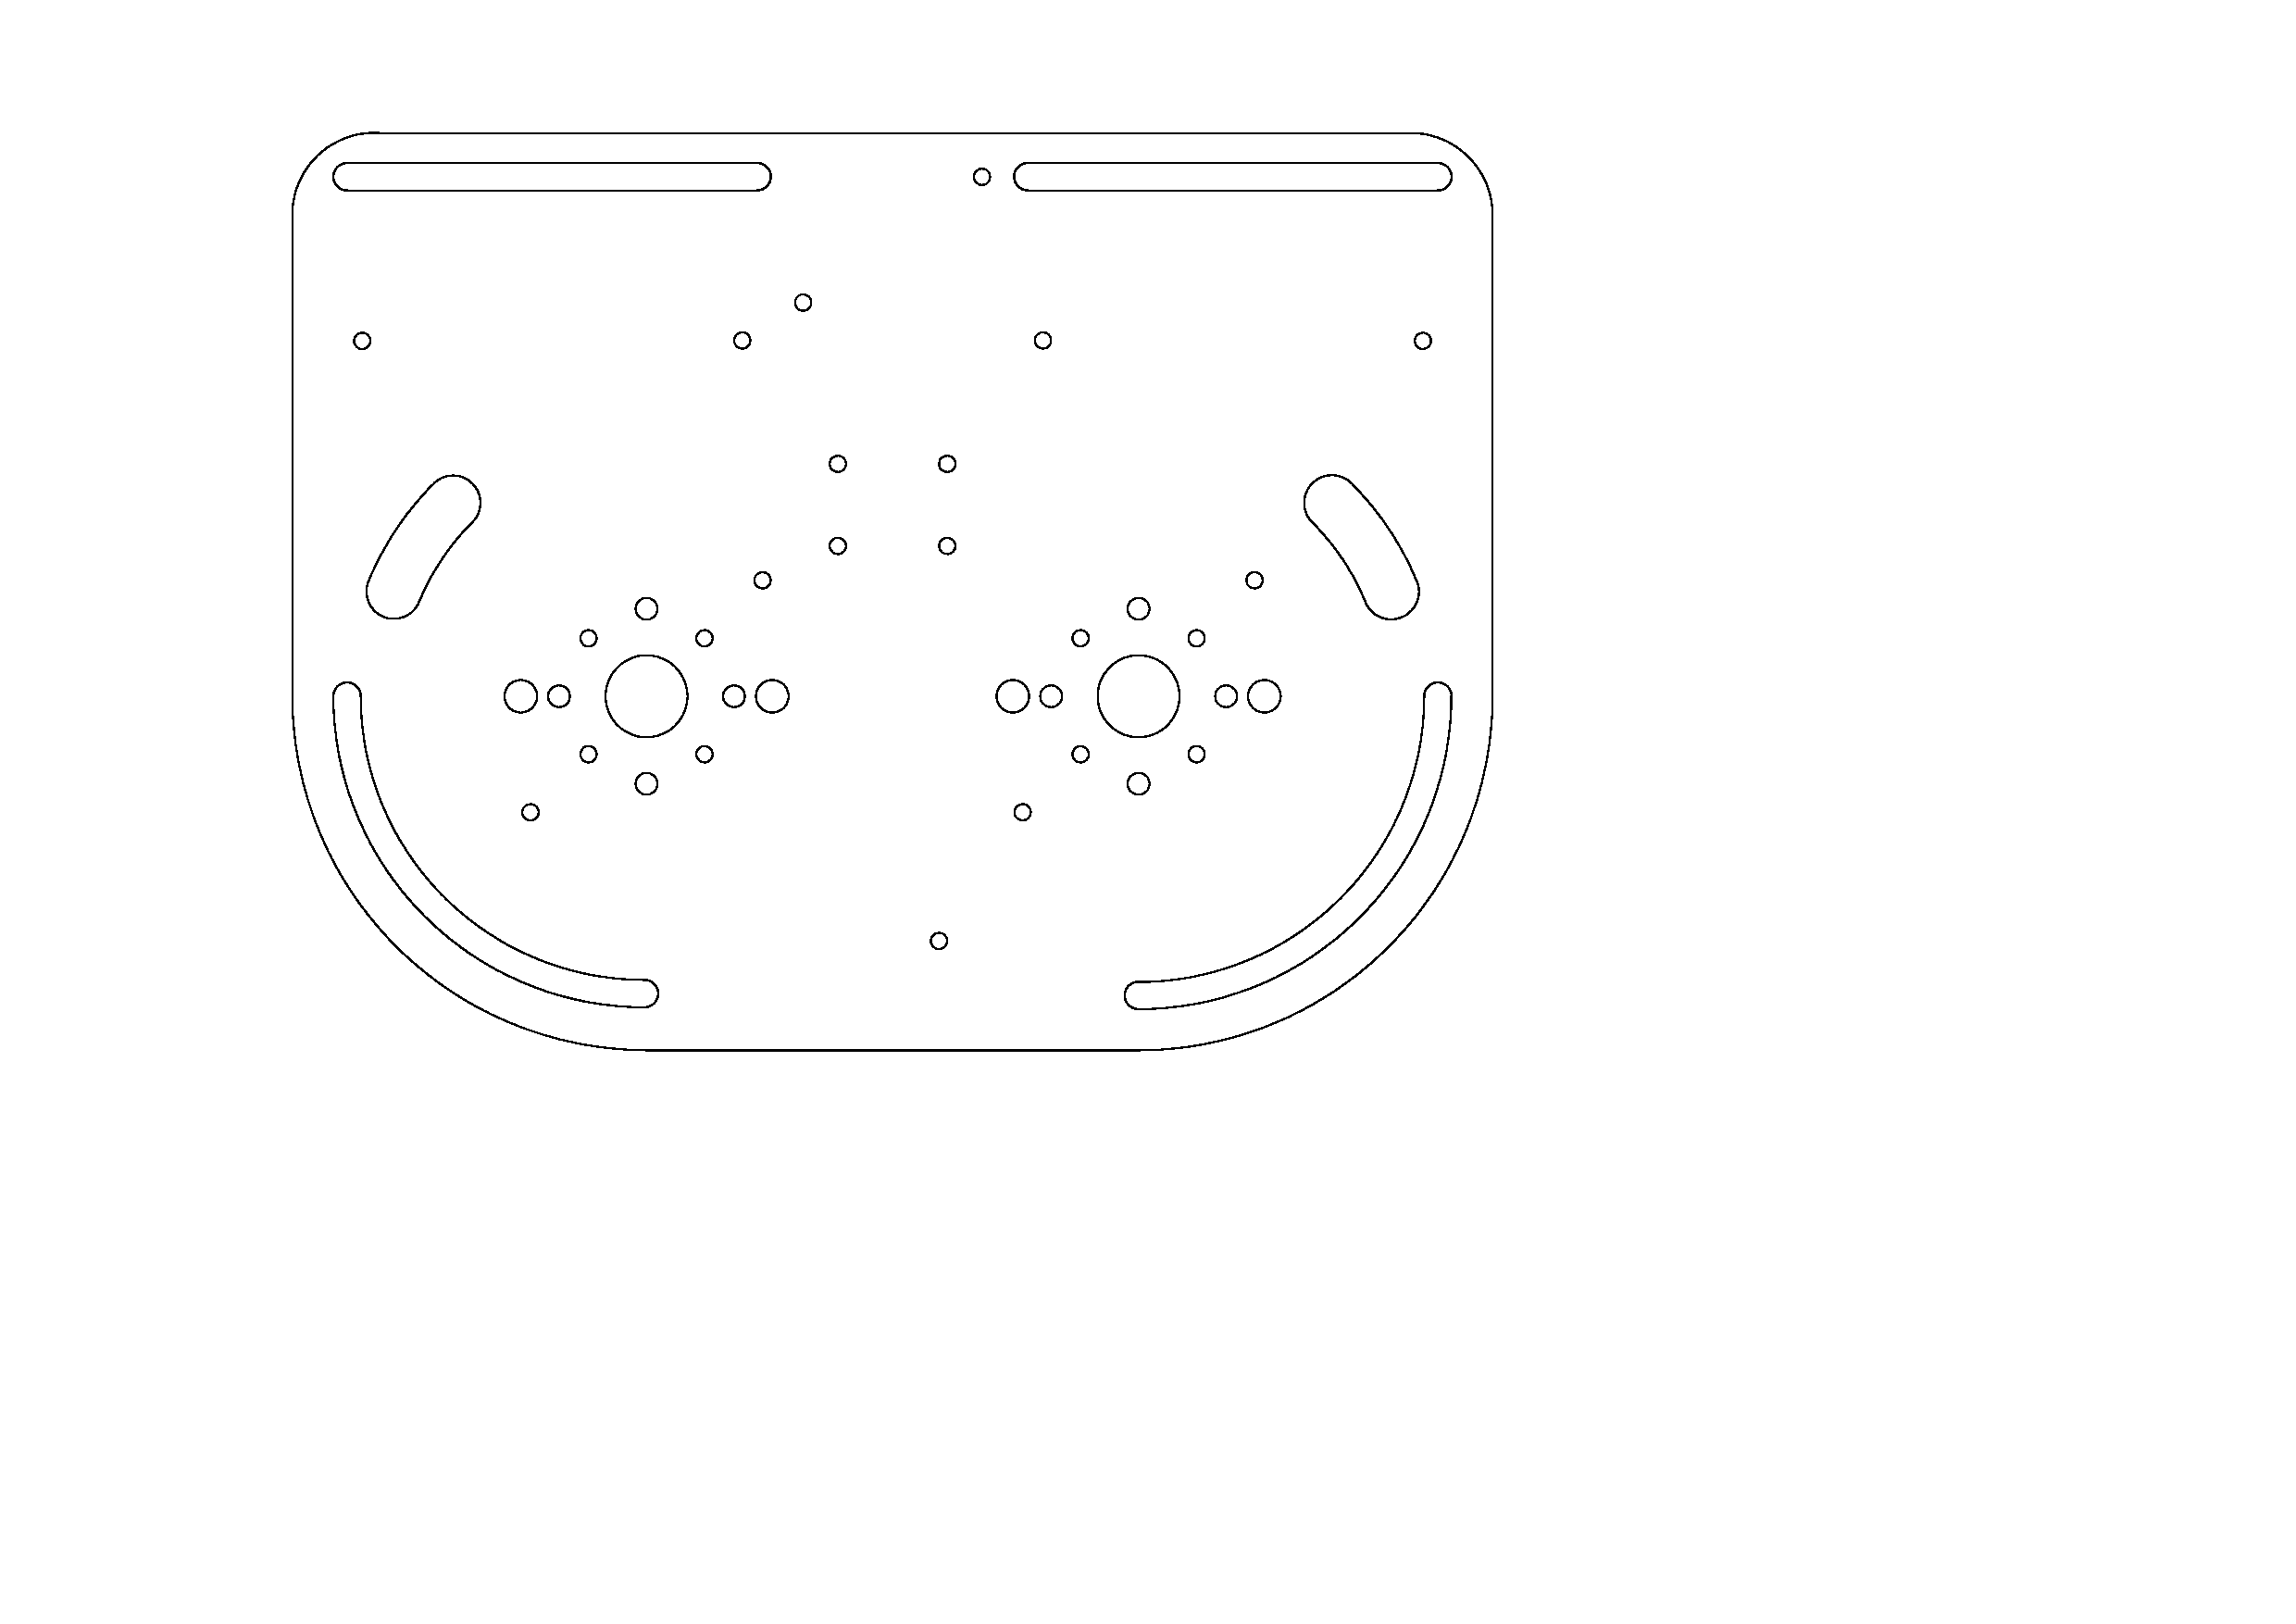
\includegraphics[clip, trim=5cm 10cm 14cm 2cm, page = 1, width=0.3\textwidth]{images/mechanical/laser-test-print-V313} 
\label{fig:CAD mounting plate V3.1.3}
}

\subfloat[][CAD mounting plate final design.]{
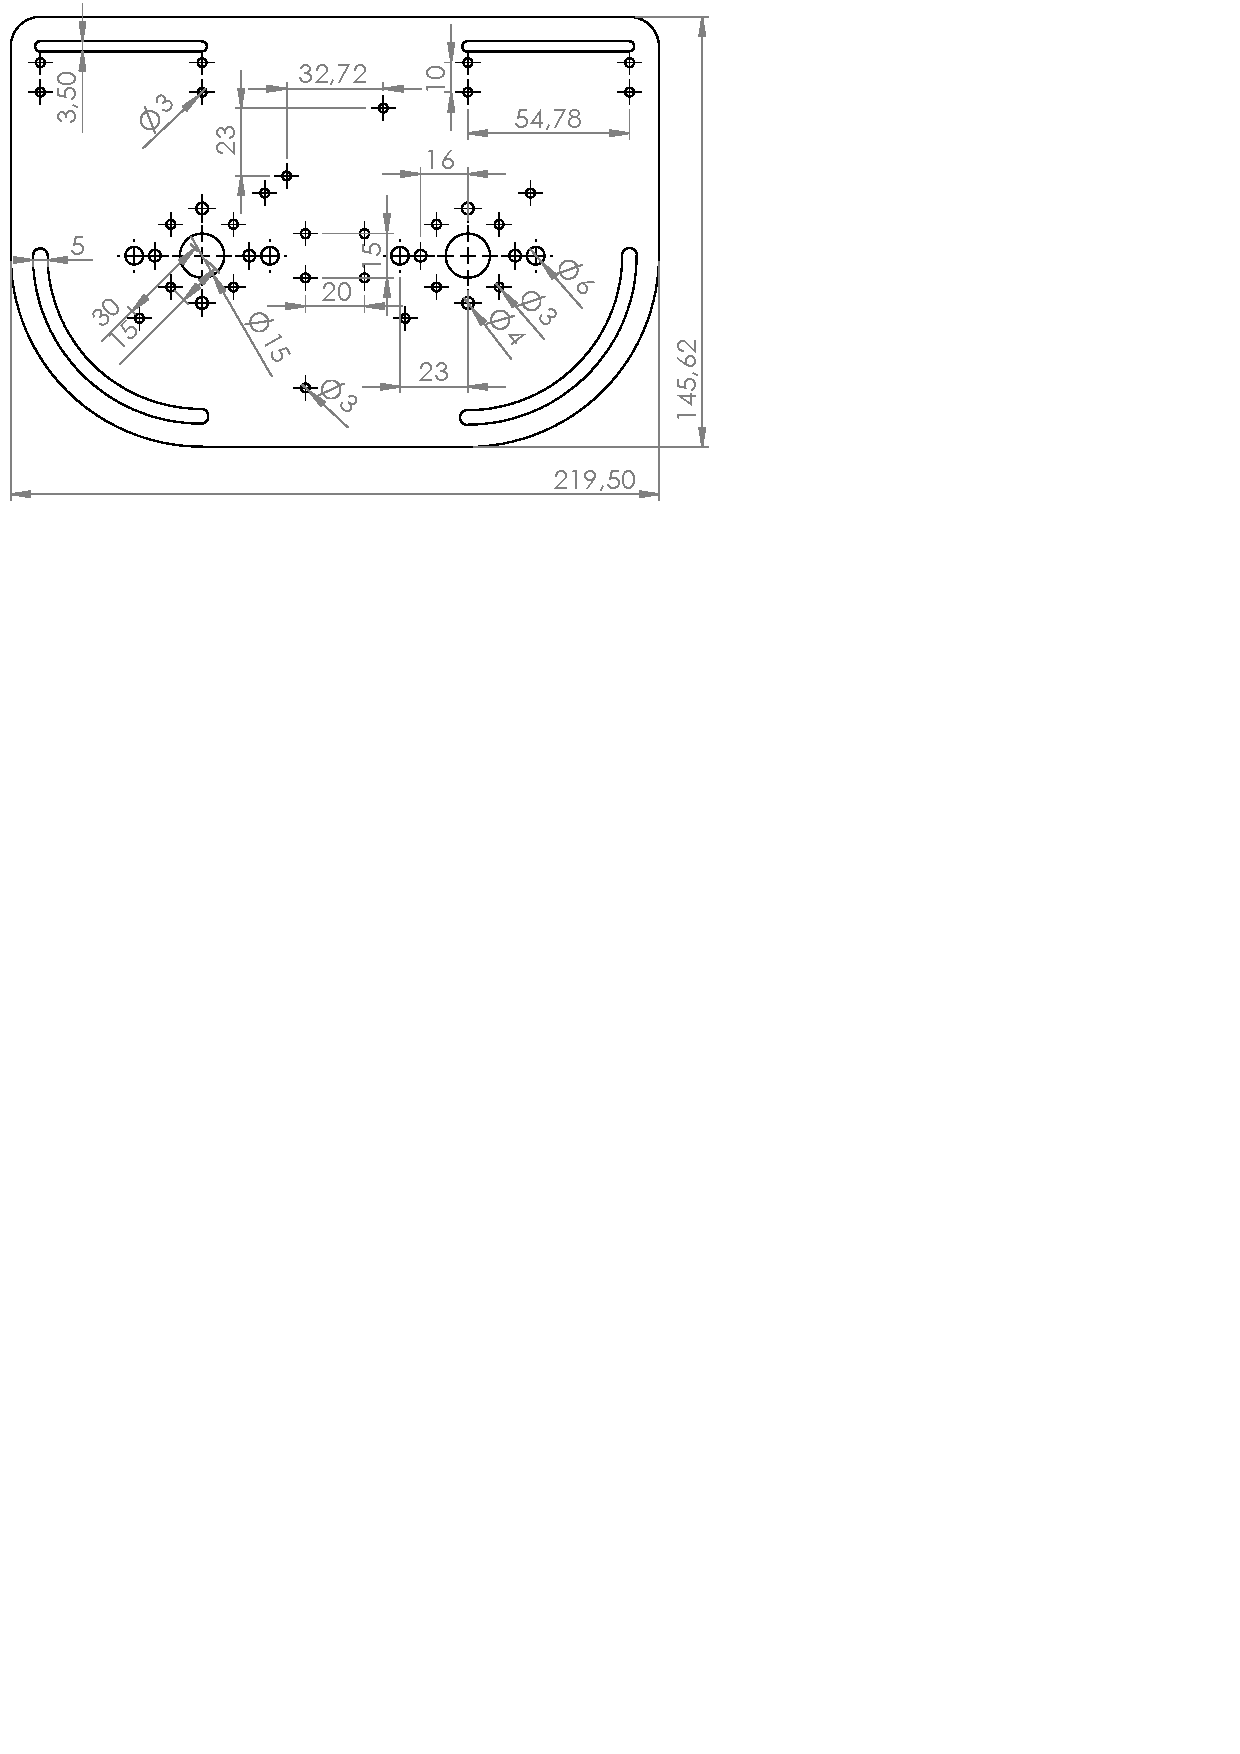
\includegraphics[clip, trim=0cm 21cm 9cm 0cm, page = 1, width=0.6\textwidth]{images/mechanical/main-plate-final} 
\label{fig:CAD mounting plate final design}
}
\caption{Leg mounting plate iterations.}
\label{fig:Leg mounting plate iterations}
\end{figure}

\begin{figure}
\centering
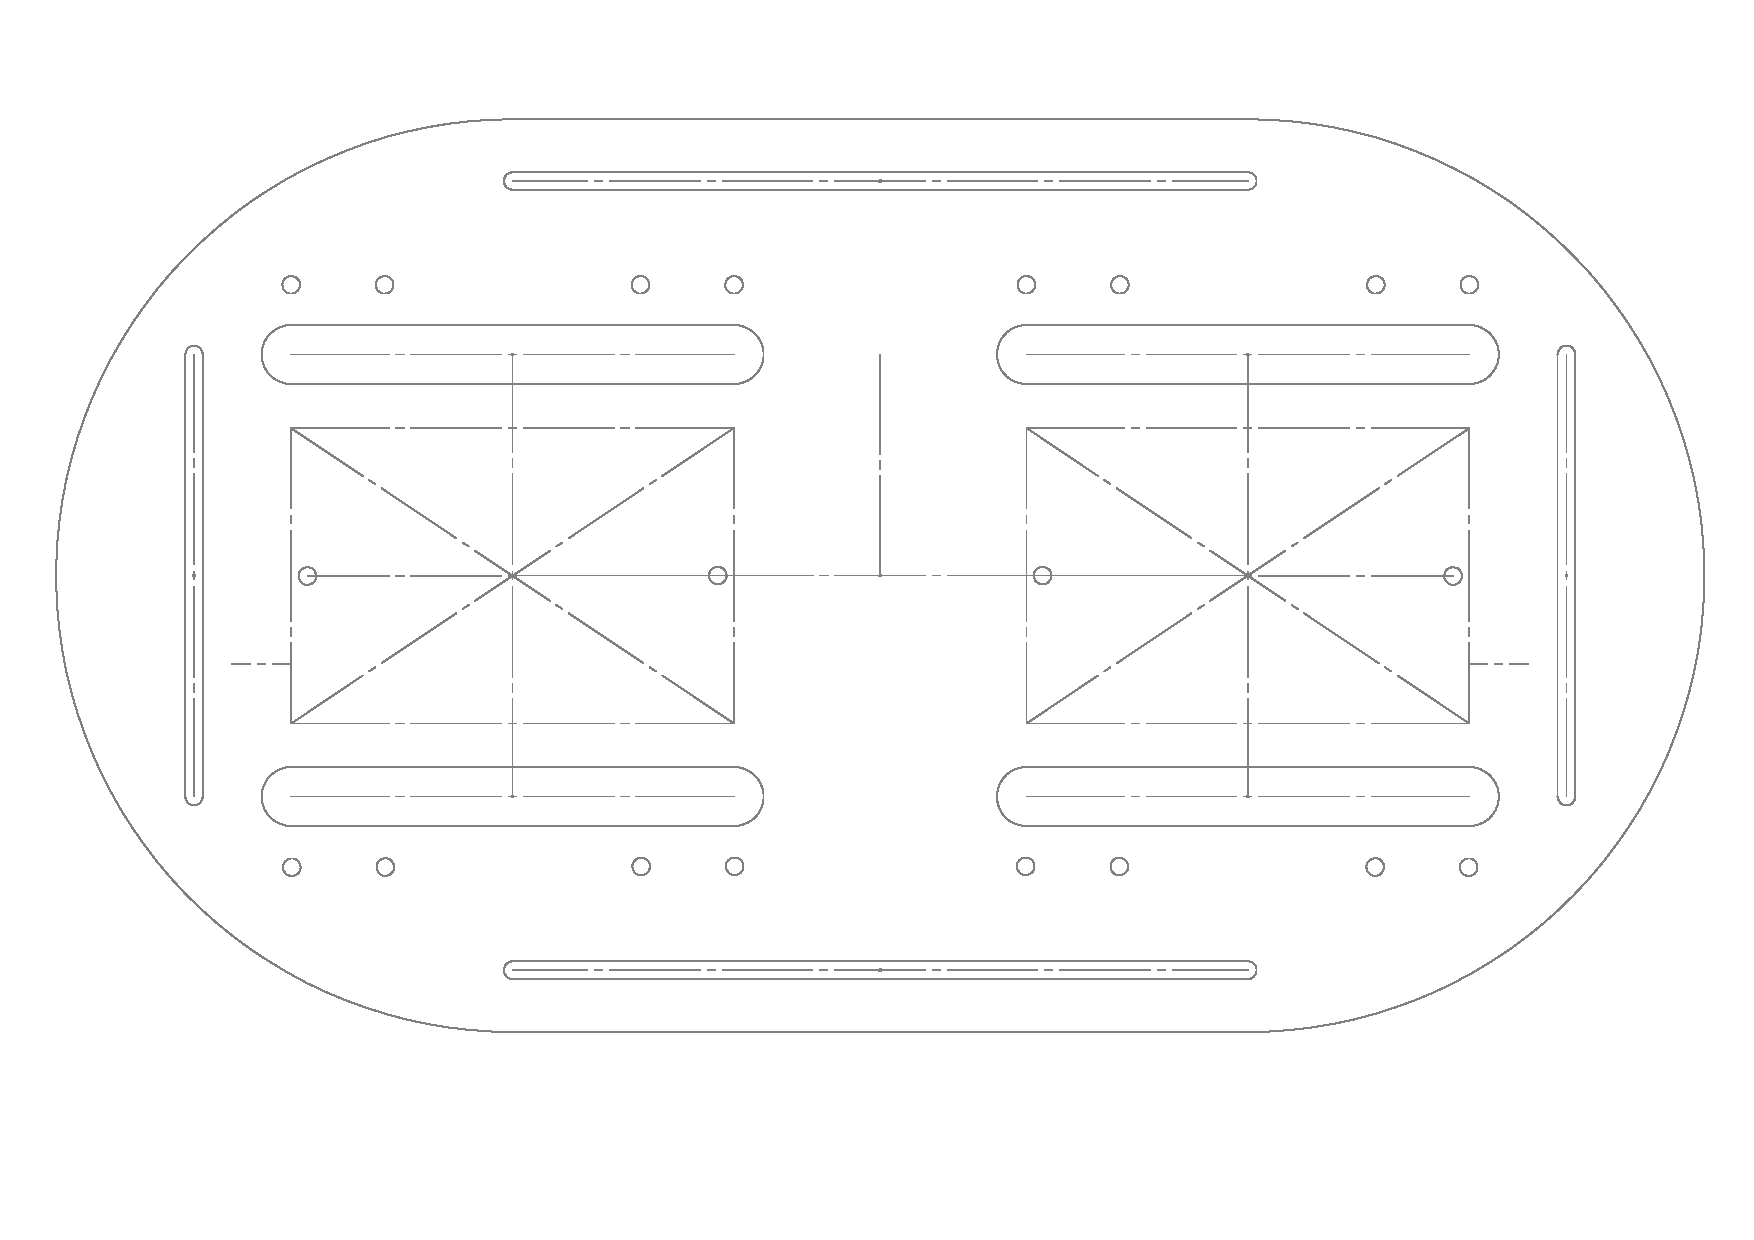
\includegraphics[width=0.6\textwidth]{images/mechanical/driver-mount-plate.pdf} 
\caption{Motor driver interface mounting plate.}
\label{fig:Motor driver interface mounting plate}
\end{figure}

\subsection{Leg Linkage and Foot Design}

The 4-bar linkage design of the leg was originally constructed by Ben Bingham in 2016 for completion of his undergraduate engineering vacation work in the mechatronics lab. The leg was constructed as follows:

\begin{itemize}
\item Three sets of rotational joints make up the linkage system. The joints were 3D printed using ABS plastic and used 3 mm screws to connect to the aluminium leg sections.
\item 8 mm loctite nut, bolt and washer combinations connected the joint components with perspex discs to reduce friction between the joints.
\item The aluminium leg sections were constructed of 25 mm diameter tubing to form a leg of 0.15 m and 0.3 m sections including the joints. 
\end{itemize}

The leg had a number of design flaws that will be improved upon in the implementation of the Mechatronics Lab Cheetah project with the leg being redesigned by Callen Fisher. These issues are listed below:

\begin{enumerate}
\item The joints provide significant friction when under torque outside of the two degrees of freedom of the leg. 
\item The resistance to movement provided by the joints in normal operation is directly related to the amount of torque tightening on the nut and bolt. 
\item The nuts and bolts slowly work themselves loose under normal operation due to vibrations and impact.
\item The motor joints, being off-set from the motor shafts, place significant torque on the motor shafts under impact.
\end{enumerate} 

Without the proper material to provide friction during foot placement on the ground, lateral slipping occurs as seen in \cref{fig:foot-slipping}. To improve the grip of the foot, the following design choices were made:

\begin{enumerate}
\item 80 to 120 grit sandpaper was placed on the platform to emulate the material encountered by a Cheetah in normal operation, namely dirt and gravel.
\item A rubber mould was made, by mixing and setting rubber components, before being attached to the foot using 3 mm hex screws.
\end{enumerate}

The combination of sandpaper and rubber foot stopped lateral slipping from occurring.

\begin{figure}
\centering
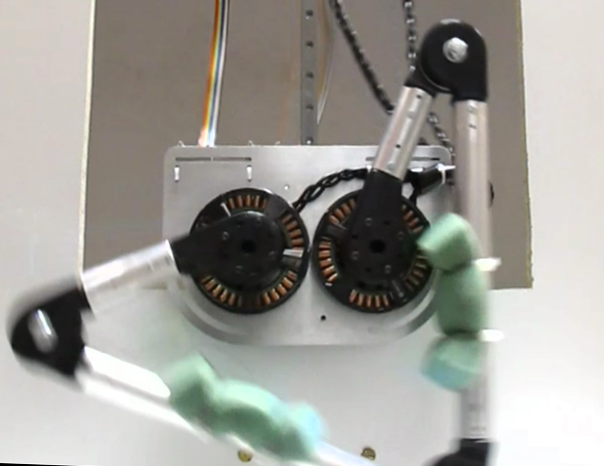
\includegraphics[width=0.6\textwidth]{images/experiments/lateral-slipping} 
\caption{Leg foot lateral slipping.}
\label{fig:foot-slipping}
\end{figure}

\subsection{Testing Platform}
\label{subsec:Testing Platform}

The testing platform was designed to be limited to a vertical axis of movement. This allows robust testing of the hopping capabilities of Baleka. In future experimentation a rotational hinged platform can be used to test forward hopping trajectories. 

The original platform design used two parallel $16\ mm$ tool steel rods with ball bearings attached to the leg platform. This not only added extra weight, but also made it difficult to properly mount the rods parallel to avoid friction. 

The original setup was replaced with an igus linear guide as seen in \cref{fig:drylin-linear-guide}, specifically the TW-04-12 DryLin T miniature slide carriage along with the appropriate rail.

A rail of $0.6\ m$ was used which resulted in a potential hopping height of $0.4\ m$. This height proved to be adequate given the motor driver's $60\ A$ current limit which in practise resulted in a maximum hopping height of just under $0.4\ m$. Further hopping experiments performed with the linear guide platform can be seen in \cref{chap:Experimental Testing}.

The linear guide rail was mounted on a wooden frame with a heavy $3\ kg$ wooden counterweight on the base. The choice of wood for the frame was to reduce vibrations and for ease of construction. The heavy wooden base ensured the platform was stable during jump experimentation.

Despite specifications of the rail not requiring lubrication, a basic oil based lubricant was used and significantly reduced friction caused by forward rotational torque of the carriage on the linear guide rail.

To simulate the environment and platform used in the hopping experiments a CAD assembly was generated, as seen in \cref{fig:Linear guide mounted leg model}, as well as a virtual world Matlab model. This allowed the leg to be manipulated and dropped on the platform to see how it would behave. The resulting tests ensured the testing platform would have a good chance of performing well in real life experiments. Given that the linear guide system was a significant capital investment this was necessary.

\begin{figure}
\centering
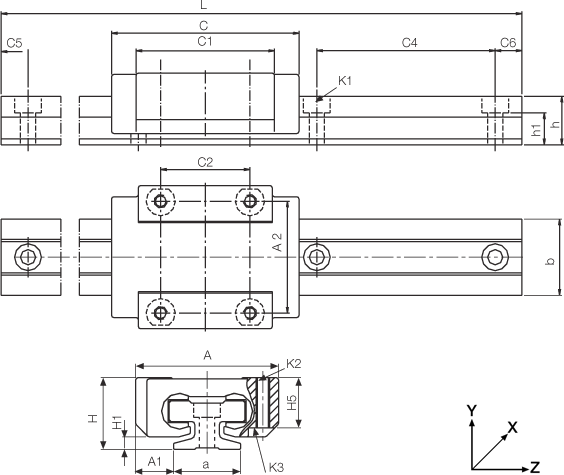
\includegraphics[width=0.6\textwidth]{images/mechanical/drylin-linear-guide.png} 
\caption{igus DryLin T - Low-profile linear guide.}
\label{fig:drylin-linear-guide}
\end{figure}


\begin{figure}
\centering
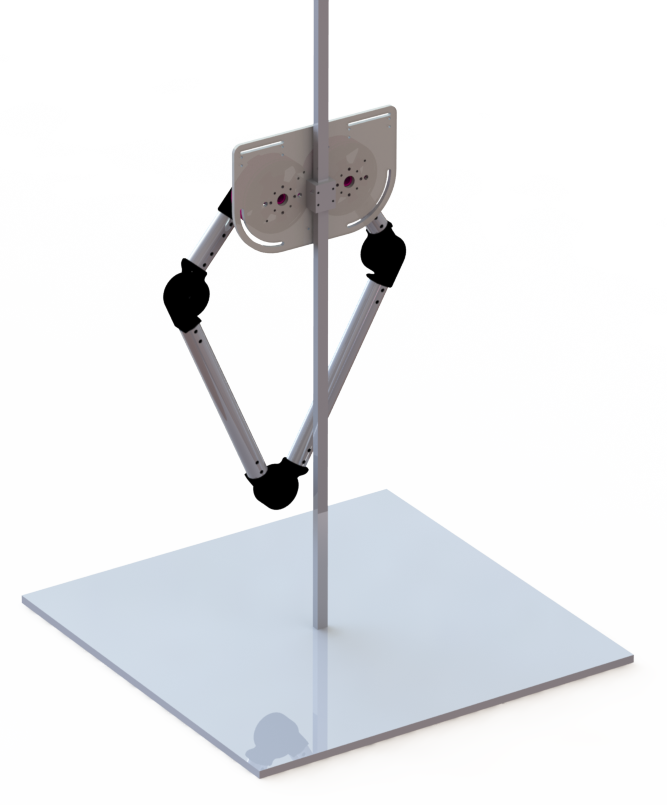
\includegraphics[width=0.4\textwidth]{images/mechanical/back-shot.png} 
\caption{Linear guide mounted leg model (CAD Solidworks assembly).}
\label{fig:Linear guide mounted leg model}
\end{figure}

\section{Mass Distribution}

The calculation of the mass and center of mass (COM) was critical for making the following design choices:

\begin{itemize}
\item Placement of the iNemo sensor board as close to the COM as physically possible (seen in \cref{fig:Final leg design - back}).
\item Mounting of the linear guide carriage as close to the COM to minimize torque and stress placed on guide rail during jumping, as well as interference to jump dynamics (seen in \cref{fig:Final leg design - back}).
\item Calculation of jump dynamics as in \cref{chap:Dynamic Modelling}.
\end{itemize}

The mass of individual leg components was first calculated manually using a scale, the log of which can be seen in \cref{tbl:Leg component mass}. The total mass of $2.2\ kg$ from this log was used in all dynamics, modelling and simulation calculations. 

The iNemo and linear guide carriage are of minimal mass and were not included in the manual mass calculation.

The center of mass was simulated in Solidworks. The material properties of each component were first configured appropriately. 

For simulation the leg radial set-point was set to $0.3\ m$ - this is the value of the leg radius during flight, freefall, impact, and compliant landing phases of jumping as seen in \cref{sec:Jump Test}. This ensures the COM calculation is accurate for the majority of the jump. 

In reality the center of mass (COM) moves negligibly with the foot position. The reason for this can be seen in \cref{fig:Mass distribution of leg assembly} where the mass distribution simulation shows the majority of the mass is concentrated around the COM, in red. The colour legend in \cref{tbl:Solidworks leg assembly mass distribution} explains the colour code and shows the simulated mass of each component.

In \cref{fig:Mass distribution of leg assembly} the COM is clearly shown as a black and white checker board circle with the distance from critical points shown on the second figure. The linear guide carriage is mounted just above this point along with the iNemo mounted with spacers above the carriage - it was not possible, due to the motor mounts, to place these components physically closer.

\subsection{Limitations}

The COM was only calculated in the two dimensional case. A significant torque was found to exist in the third dimension during experimentation that caused the leg to twist forward on the mount. This provided significant friction on the linear guide rail. In future designs the COM should be calculated in the third dimension and the motors possibly mounted coaxially on either side of the aluminium plate - this would have minimized the forward torque as the motors are the components with the most mass.

\begin{table}[]
\centering
\begin{tabular}{llll}
\textbf{Item}             & \textbf{Mass (g)} & \textbf{No.} & \textbf{Total Mass (g)} \\
T-Motor U10 Plus          & 500               & 2            & 1000                    \\
Servo drive               & 123.9             & 2            & 247.8                   \\
Servo drive mounting card & 50.7              & 2            & 101.4                   \\
Leg                       & 500               & 1            & 500                     \\
Plate                     & 350               & 1            & 350                     \\
\textbf{Total}            & \textbf{}         & \textbf{}    & \textbf{2199.2}        
\end{tabular}
\caption{Leg component mass.}
\label{tbl:Leg component mass}
\end{table}

% Please add the following required packages to your document preamble:
% \usepackage[table,xcdraw]{xcolor}
% If you use beamer only pass "xcolor=table" option, i.e. \documentclass[xcolor=table]{beamer}
\begin{table}[]
\centering
\begin{tabular}{llll}
\textbf{Colour legend}                          & \textbf{Component}    & \textbf{No.} & \textbf{Mass (g)} \\
\cellcolor[HTML]{FE0000}                        & T-Motor U10 Plus      & 2            & 424.56            \\
\cellcolor[HTML]{CB0000}                        & Mounting Plate        & 1            & 378.86            \\
\cellcolor[HTML]{010066}{\color[HTML]{000000} } & Linear Guide Carriage & 1            & 100.37            \\
\cellcolor[HTML]{3531FF}                        & ABS Motor Joint       & 2            & 50.55             \\
\cellcolor[HTML]{3531FF}                        & Long Linkage          & 2            & 46.40             \\
\cellcolor[HTML]{3531FF}                        & Joint                 & 5            & 39.83             \\
\cellcolor[HTML]{3531FF}                        & Foot Joint            & 1            & 39.63             \\
\cellcolor[HTML]{3531FF}                        & Short Linkage         & 2            & 12.81             \\
\cellcolor[HTML]{3531FF}                        & Washer Bearing        & 3            & 2.41              \\
\textbf{Total:}                                 & \textbf{}             & \textbf{}    & \textbf{1793.88} 
\end{tabular}
\caption{Solidworks leg assembly mass distribution.}
\label{tbl:Solidworks leg assembly mass distribution}
\end{table}

\begin{figure}
\centering
\subfloat[][Mass distribution simulation.]{
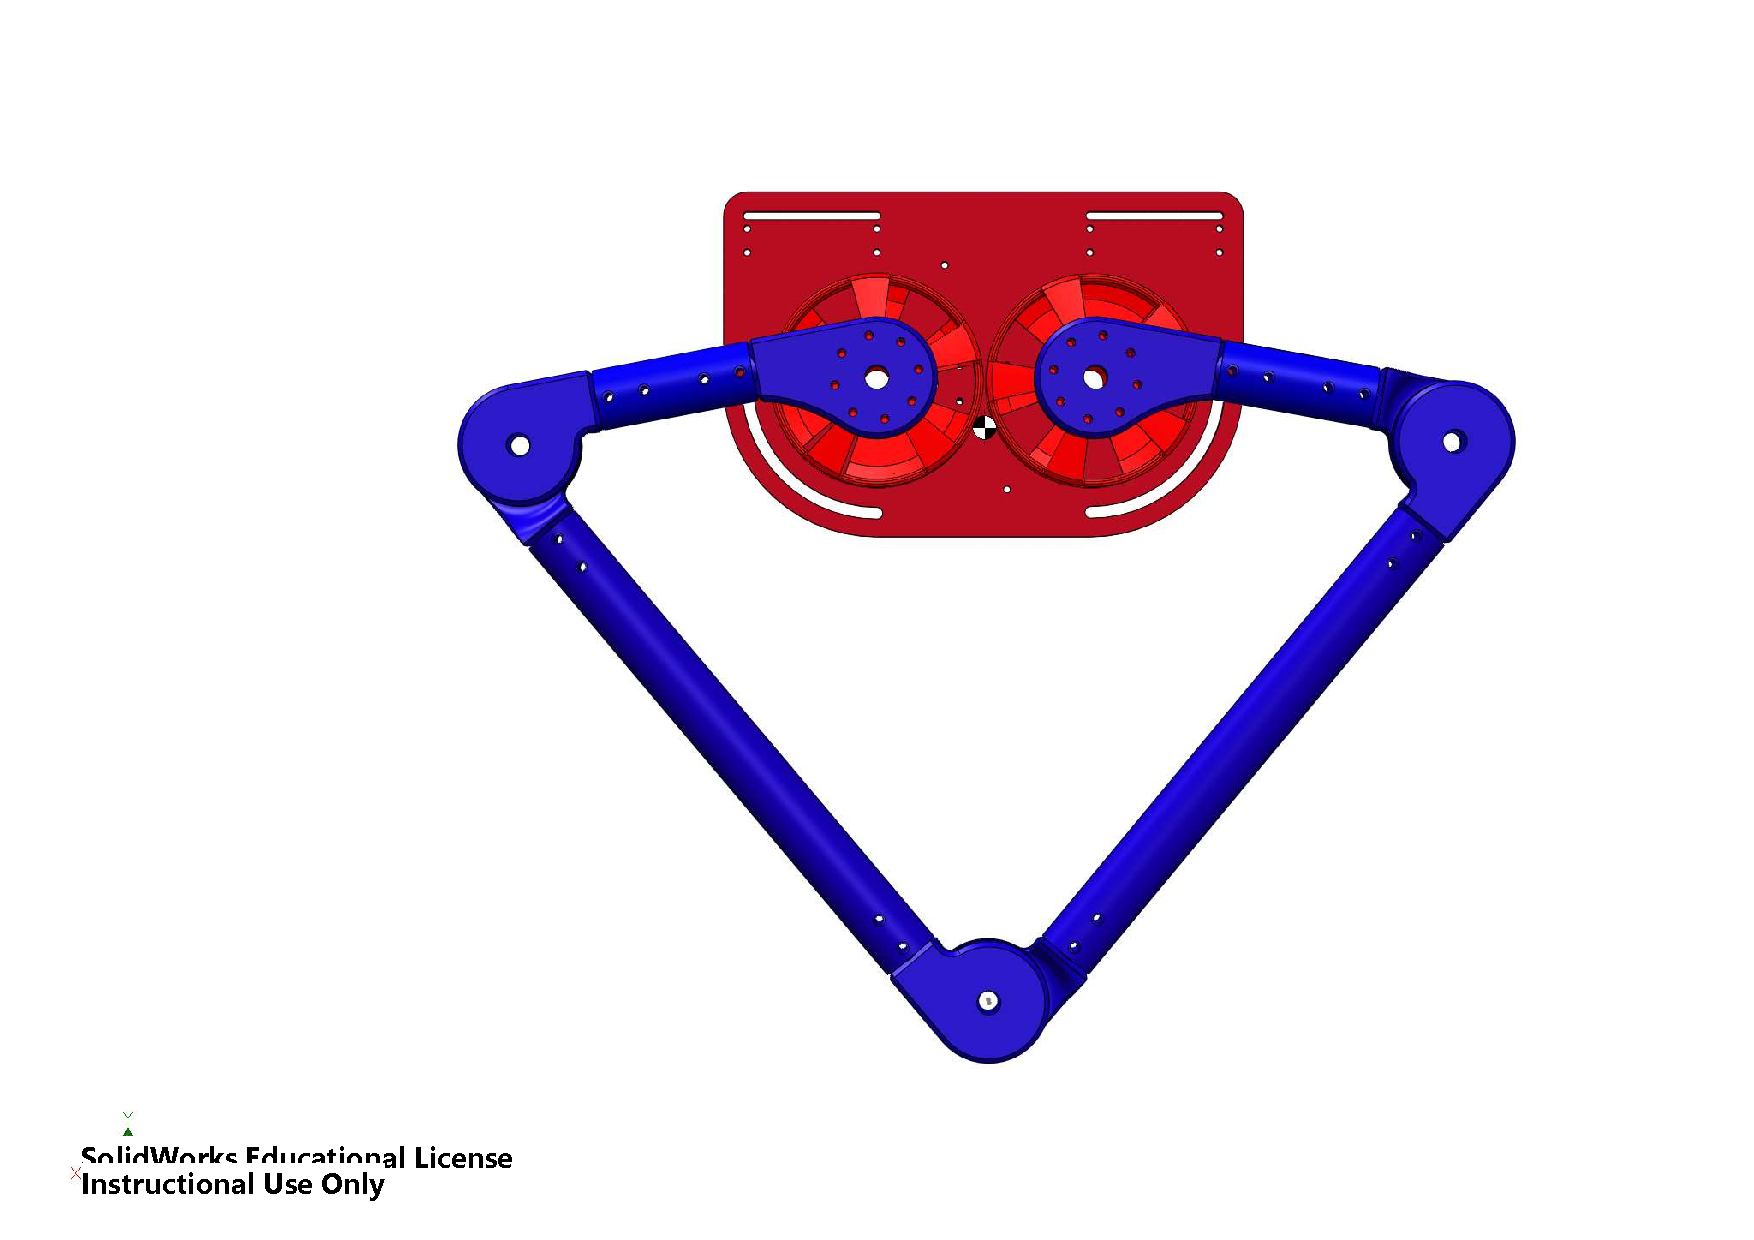
\includegraphics[clip, trim=5cm 2cm 4cm 2cm, page = 1, width=0.7\textwidth]{images/mechanical/assembly-com-distribution.pdf} 
}
%\subfloat[][Mass distribution colour legend (grams).]{
%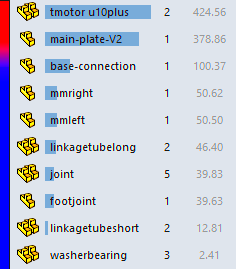
\includegraphics[width=0.3\textwidth]{images/mechanical/com-distribution} 
%}

\subfloat[][Center of mass of leg assembly.]{
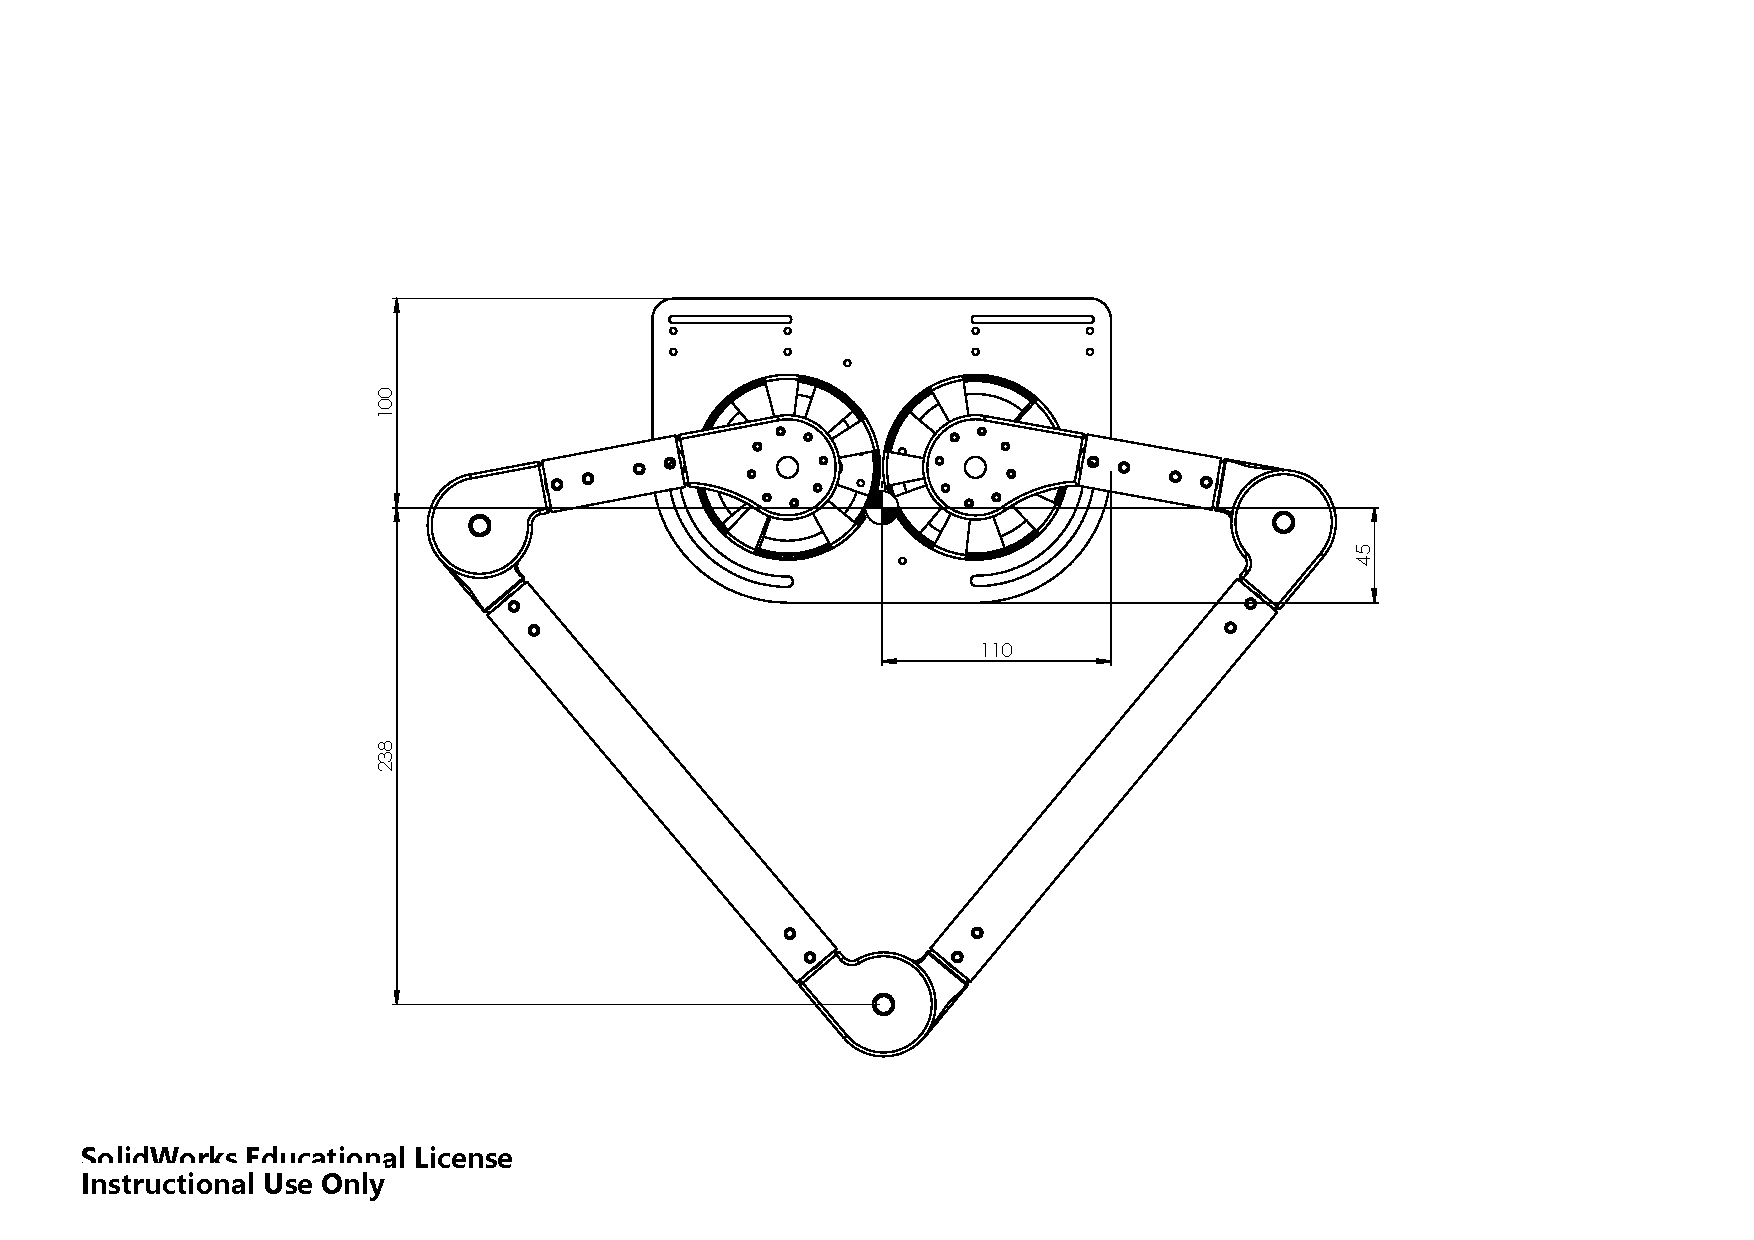
\includegraphics[clip, trim=5cm 2cm 5cm 5cm, page = 1, width=1\textwidth]{images/mechanical/assembly-com.pdf} 
}
\caption{Mass distribution of leg assembly.}
\label{fig:Mass distribution of leg assembly}
\end{figure}

\subsection{Actuator to Body Mass Ratio}
In the study \cite{Kenneally2016} it is stated that as large a proportion of the mass budget as possible should be dedicated to the actuator, in this case the T-Motor U10 Plus BLDC motor. \Cref{tbl:Robot performance comparison} shows that the Baleka robotic leg has the second highest actuator to body mass ratio, second only to the GOAT leg. This performance rating is perhaps biased as the Baleka leg does not have the mass of on-board motor drivers and control.

\section{Mechanical Impedance}
\label{sec:Mechanical Impedance}
\subsection{Linear Guide}

In \cref{sec:Jump Test} a set of jump-tests were performed. By extracting the acceleration data from the video frames of a jump a plot of acceleration vs. time was found as seen in \cref{fig:acc-time-jump}. During the free-fall phase of the jump the mean acceleration was calculated as $-9.51\ m/s^2$. Using this acceleration and the known acceleration due to gravity, the coefficient of kinetic friction for the linear guide, $\mu_k$, can be calculated as in \cref{eq:linear-guide-friction}.  

\begin{equation} \label{eq:linear-guide-friction}
\begin{aligned}
&F_k = F_n \mu_k \\
&\mu_k = \frac{F_k}{F_n} \\
&\mu_k = \frac{|m\ddot{x} - mg|}{|mg|} \\
&\mu_k = \frac{|2.2\times -9.51 - 2.2\times -9.81|}{|2.2\times -9.81|} \\
&\mu_k = 0.031
\end{aligned}
\end{equation}

This value for kinetic friction is minimal and in practise was assumed to have an insignificant effect on jump dynamics. If a more precise mechanical system was developed and jump height control was implemented, then the kinetic friction could be taken into account. In experimentation the jump height was not consistently controllable due to mechanical joint slack.

\subsection{Leg and Joints}

The friction, and to a limited extent the inertial load, of the leg and joints was accounted for during the calibration process for the torque constant $K_t$ in \cref{sec:Motor Model Calculations}. By using force control and the calibration process the joint frictional force that needs to be overcome is indirectly included in the control model.

Due to mechanical joint slack and an imprecise mechanical system, as discussed previously, the inertial and precise frictional load of the leg is difficult to accurately calculate - because of this it is better to experimentally account for all these factors during calibration.

\section{Electronics and Communication}
\subsection{Accelerometer and Gyroscope}

The iNemo board designed and built by Callen Fisher during his masters studies, consisting of a STM32F1 microcontroller with on-board accelerometer, gyroscope and magnetometer, was to be used to measure acceleration data for force measurements and jump phase control. 

Due to time constraints acceleration data was not used or found to be necessary for basic hopping control. Provision was made for mounting the board as close to the center of gravity of the robot as was physically possible, as can be seen in \cref{fig:Final leg design - back} where the final mounting setup is shown. 

The iNemo board was mounted approximately $4\ cm$ from the center of gravity directly over the linear guide. This was achieved by using nylon spacers and the included $3\ mm$ mounting points on the board.

The necessary peripheral configuration and data processing can be easily integrated into the embedded system communication protocol developed in \cref{chap:Software Development} in future. The GitHub page for the iNemo development board can be seen at \url{https://github.com/Callen-Fisher/INEMO-development-board}.

\subsection{Distance Sensor}
A distance sensor was mounted to the base of the mounting plate, as seen in \cref{fig:Final leg design - back}. This provided feedback of the height of the leg's center of mass above the ground.

The leg height was used for height control as well as flight phase determination.

An infra-red distance sensor was chosen with a narrow beam width - this ensures there is minimal reflection off surrounding objects that could interfere with distance readings. The beam reflects off the surface of the ground and a time-of-flight calculation is used to determine distance. Infra-red is open to possible interference from surrounding fluorescent light sources, and this can be accounted for by using it in an area out of direct line of site of light sources. Infra-red was chosen because it is cheaper than an equivalent laser distance sensor.

The Pololu Carrier with Sharp GP2Y0A60SZLF Analog Distance Sensor was used. It requires a $3\ V$ voltage source which can be supplied directly from the micrcontroller which runs off the same voltage. 

The distance sensor outputs an analog signal which is related to the height. This analog signal is fed into the ADC of the microcontroller and using a linear relationship is mapped to the distance. 

The Pololu distance sensor has a range of $10-150\ cm$, which is more than enough for the intended hopping height of $20-50\ cm$ due to the testing rig limits.

The height sensor was calibrated by setting it at $0.1\ m$ from a surface and using a scaling factor to adjust the linear relation between distance and voltage until an accurate measurement was achieved. 

A 3D printed carrier, a render of which can be seen in \cref{fig:distance-sensor-mount}, was designed for the distance sensor which offset the sensor from the mounting plate and placed it in a central location above the linear guide.

\begin{figure}
\centering
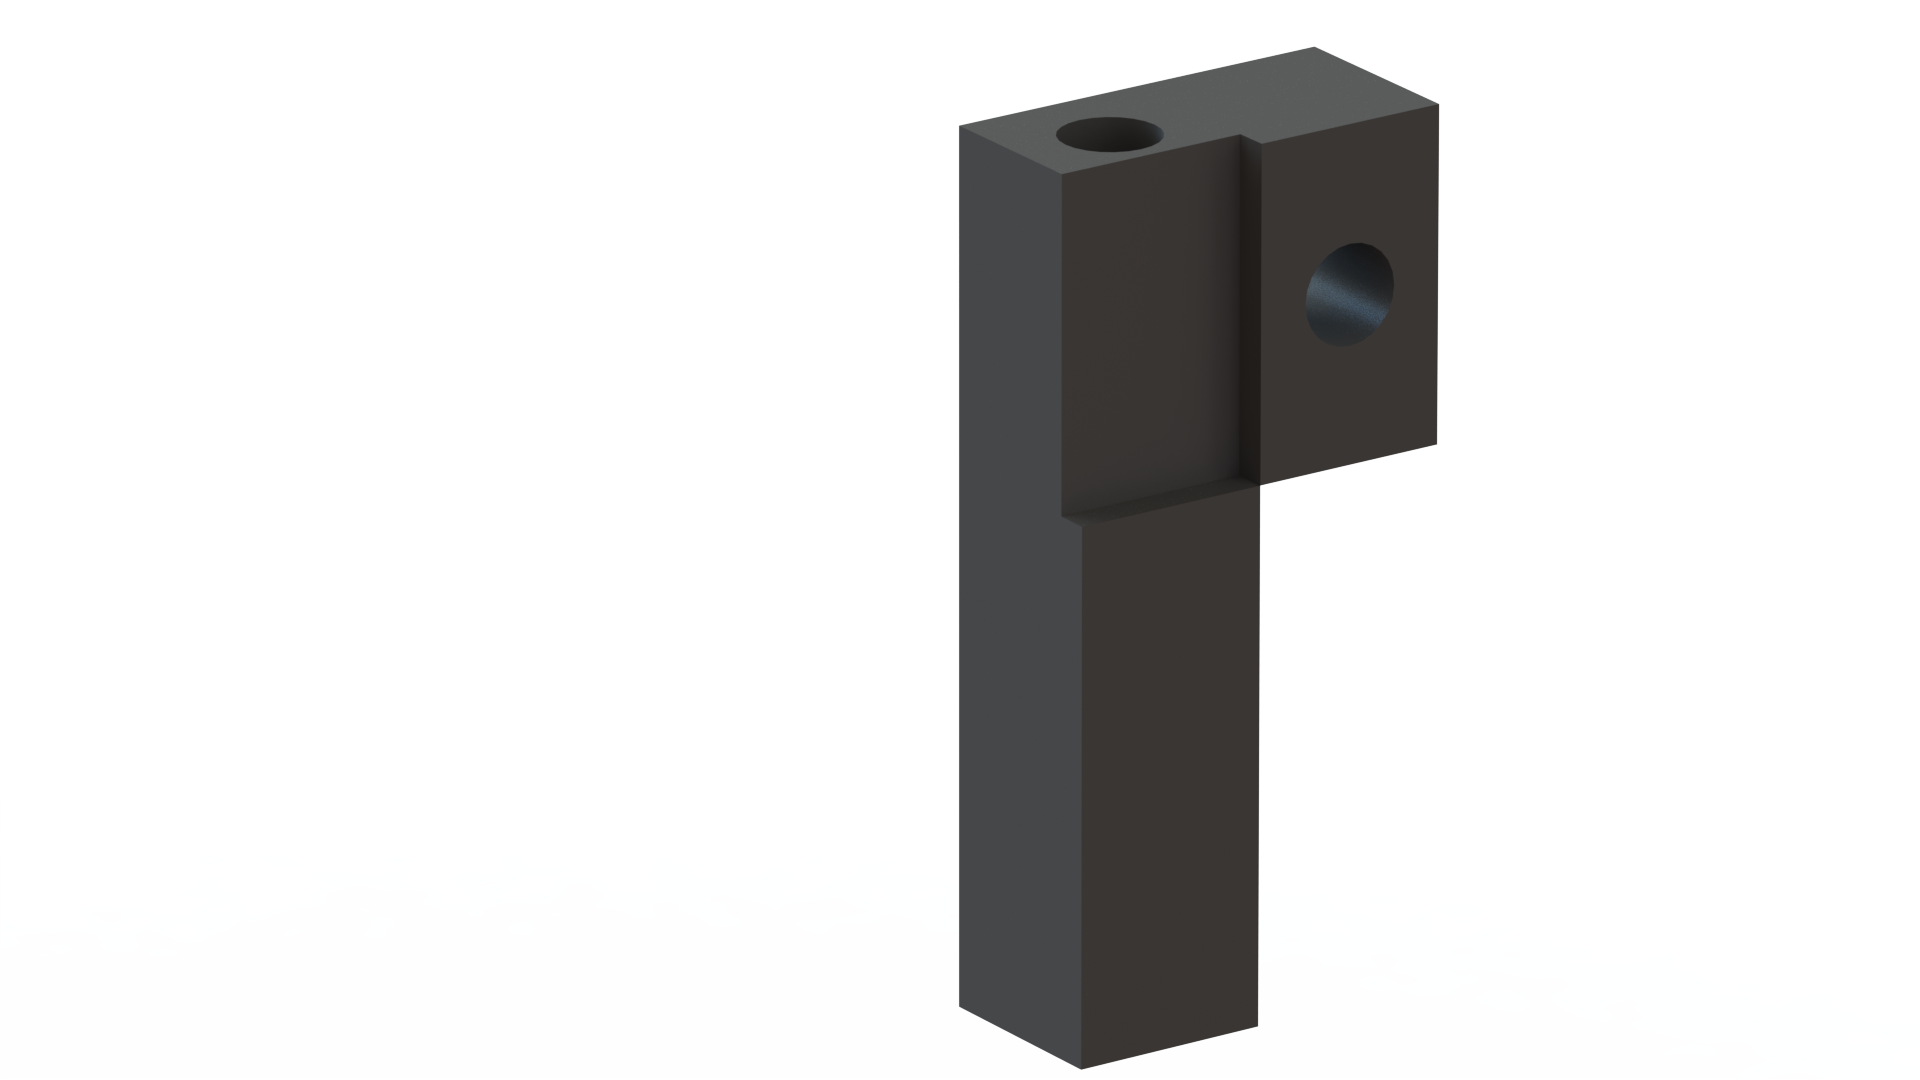
\includegraphics[clip, trim=4cm 0cm 2cm 0cm, width=0.4\textwidth]{images/mechanical/distance-sensor-mount} 
\caption{3D printed PLA distance sensor mount.}
\label{fig:distance-sensor-mount}
\end{figure}

\subsection{Microcontroller}
The microcontroller had to meet the following specifications:
\begin{itemize}
\item 4 x UART Ports
\item 1 x ADC
\item 1 x Floating point unit
\item DMA Capabilities
\item USB Debugging
\item 5V tolerant UART ports
\end{itemize}

Being familiar with the STM32 series of microcontrollers, a STM32F4 board was chosen and met the above specifications with two additional USART ports for future peripheral needs.

\section{Motors and Drivers}

\subsection{Driver Selection}
\label{sec:Driver Selection}

The most important factor when choosing a motor driver for dynamic hopping control is the peak current specification. During the launch phase a current impulse will be used to transfer maximum energy to the flight phase. 

In \cref{fig:motor-current-requirements} the kinematic workspace developed in \cref{sec:Simulation-Kinematics} was combined with a virtual compliance control simulation to determine what the theoretical maximum current requirement would be.

A heat map for motor 1 and motor 2 current draw can be seen, with a maximum current magnitude of $52.3\ A$. This simulation was performed with a nominal virtual spring configuration of: 
\begin{itemize}
\item $K_{s1}=300\ N/m$
\item $K_{s2}=30\ N/m$
\end{itemize}
In order to account for the extra current draw when using damping, $60\ A$ was chosen as the motor driver specification. 

The peak current specification chosen was adequate for the platform in use, but for achieving higher and more fine tuned jump control a higher peak current is needed. This is further investigated in \cref{sec:Jump Test}.

To achieve a controller sampling frequency of $200\ Hz$ a high speed and robust communication protocol is needed. RS-485 was chosen as the preferred protocol for the following reasons:
\begin{enumerate}
\item Robust to noise interference from BLDC motors.
\item Can support high speed data rates up to $1\ MBaud$.
\item Easy to implement and readily available on off-the-shelf microcontrollers.
\end{enumerate}

In practise the motor drivers caused a communication bottle neck due to the time taken for the controllers to respond to control packets sent - ideally the motor driver should be able to receive, process and reply to control packets without a significant delay. This is further investigated in \cref{chap:Software Development}.

The specifications determined above were met by the AMC servo drive and mounting card seen in \cref{fig:AMC Servo Drive and Mounting Card}. 

\begin{figure}
\centering
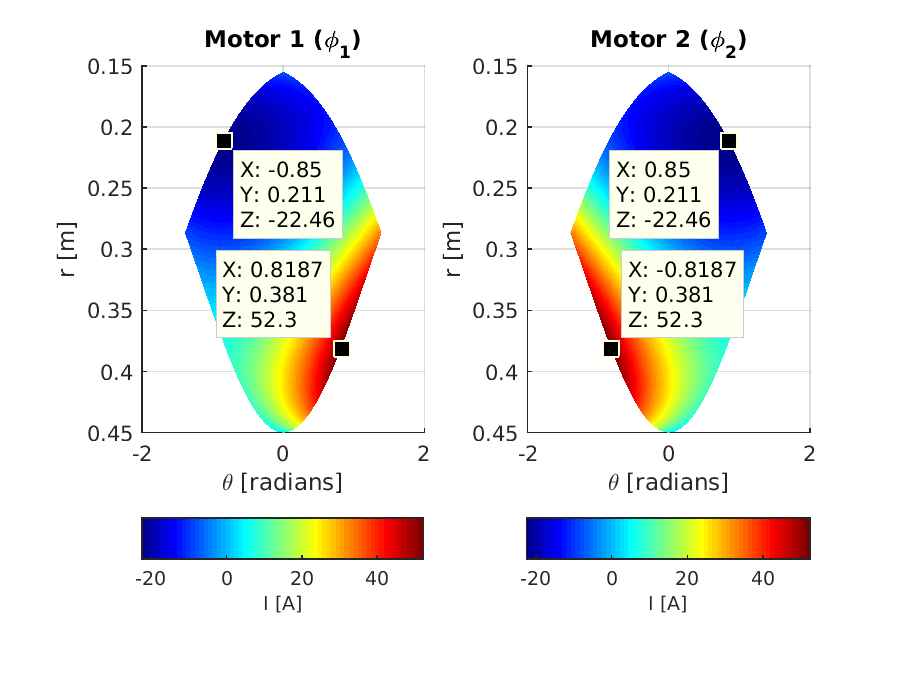
\includegraphics[width=0.8\textwidth]{images/control/forward-kinematic-motor-current.eps} 
\caption{Active compliance motor current requirements.}
\label{fig:motor-current-requirements}
\end{figure}

\begin{figure}
\centering
\subfloat[][AMC DigiFlex Performance Servo Drive.]{
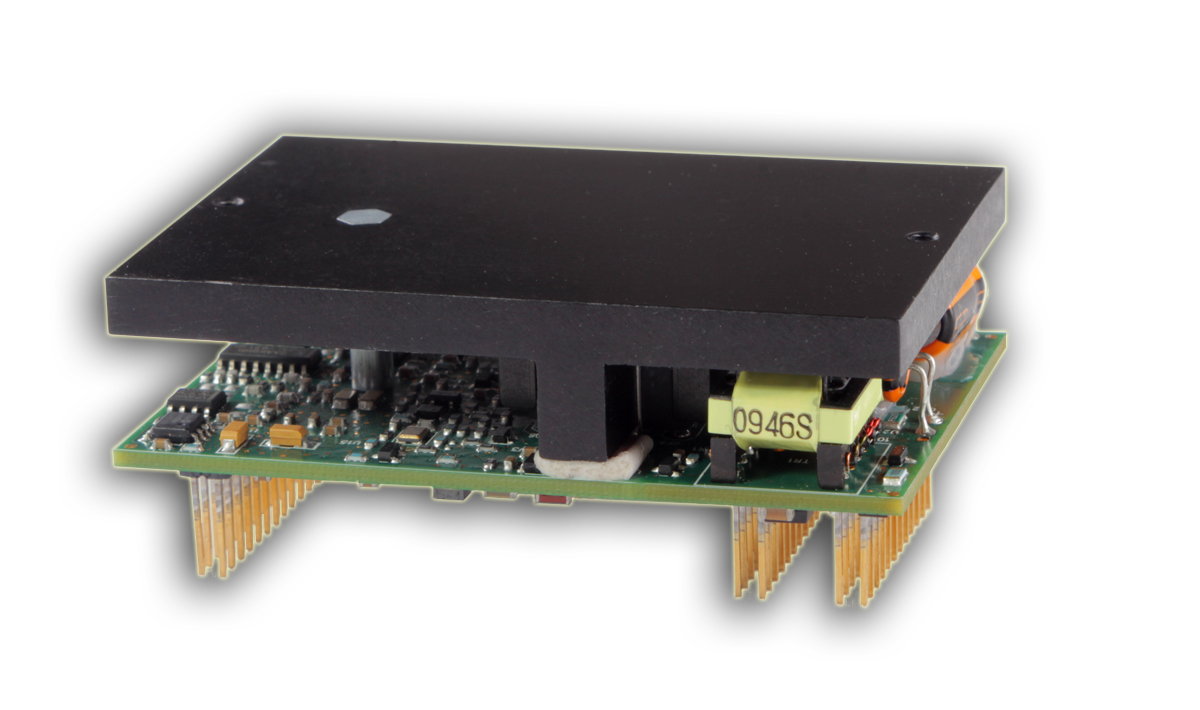
\includegraphics[width=0.3\textwidth]{images/driver/driver.jpg} 
}
\subfloat[][AMC DigiFlex Performance Servo Drive mounting card.]{
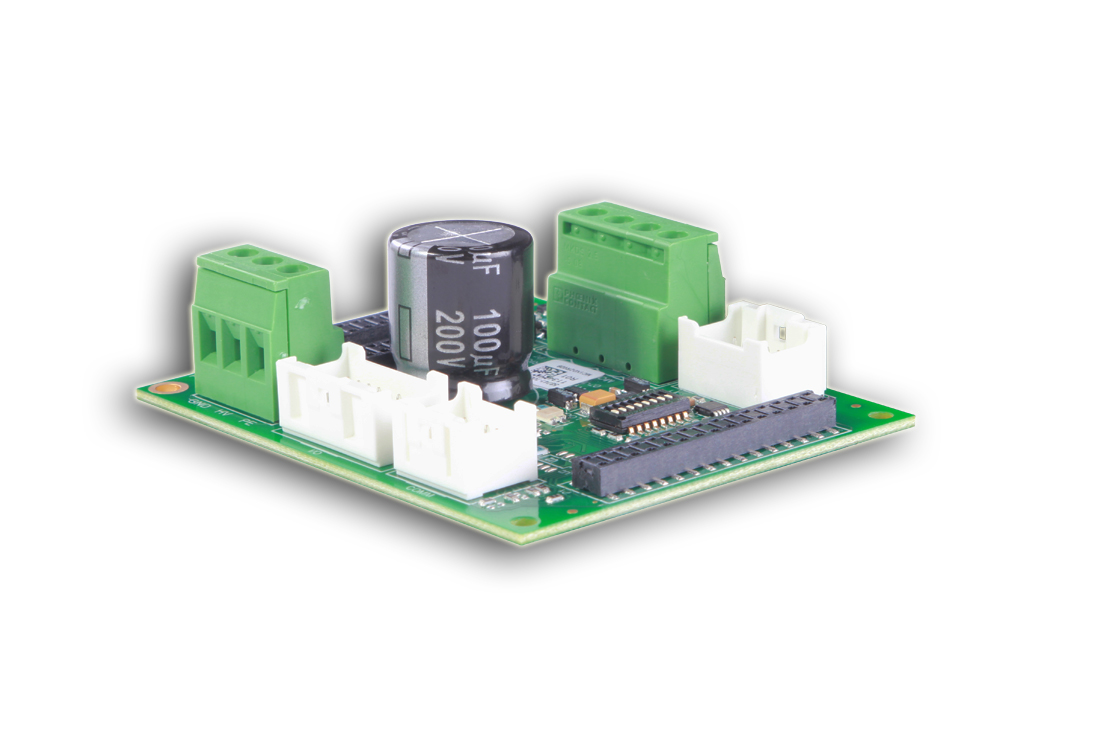
\includegraphics[width=0.3\textwidth]{images/driver/mounting-card.jpg}
} 
\caption{AMC Servo Drive and Mounting Card.}
\label{fig:AMC Servo Drive and Mounting Card}
\end{figure}

\subsection{Motor Selection}
\label{sec:Motor Selection}

A brushless DC motor (BLDC), by definition, has few parts such as brushes that will degrade over time or provide resistance to movement. This is advantageous in robotic systems were repeated high torque operations will be performed.

Due to the recent popularity of BLDC motors in use on quadcopter and other hobby platforms, high performance motors have become more accessible. 

In the case of a direct drive robotic platform, performance is measured by the amount of torque the motor can supply for a given current under load.

In the study by \cite{Kalouche2016} various COTS (commercial off the shelf) motors were compared using the thermal specific torque as a performance measure. The T-Motor U10 Plus was found to have the highest thermal specific torque at $0.42 \frac{Nm}{kgC^o } \text{ at } r_{gap} = 40 mm$ \cite{Kalouche2016}. When compared to the custom made MIT Cheetah motors at $0.71 \frac{Nm}{kgC^o } \text{ at } r_{gap} = 49 mm$ found in \cite{Wang2012} they perform favourably. 

\Cref{fig:Motor performance requirements} visually shows the relationship between torque, current and speed and places the requirements of the Baleka leg on the plot in blue and the specifications of the T-Motor U10 Plus in red. The T-Motor U10 Plus has the following specifications:

\begin{itemize}
\item KV rating: 80
\item Shaft diameter: 15 mm
\item Weight: 500 g
\item No. of Cells (Lipo): 6-14s
\item Max Continuous current(A): 33 A
\item Max Continuous Power(W): 1500 W
\item Internal resistance: $95\ m\Omega$
\end{itemize}

The KV rating of 80 indicates an unloaded speed of $80\ rpm$ per volt. This is on the low end of the scale and generally means the motor can achieve a higher torque at low speed than a higher KV rated motor.

The ideal motor for the robotic platform would achieve high torque, low current draw and a high torque for low speed operation as shown in blue in \cref{fig:Motor performance requirements}. 

The T-Motor U10 Plus sits somewhere in the middle of the performance plot, allowing relatively high speed operation using a 10s battery with adequate torque and current draw specification. Two 5s LiPos in series were used to supply the motors, providing approximately $40\ V$ and a theoretical maximum speed of $3200\ rpm$.

The T-Motor U10 Plus was chosen for the reasons above, as well as the fact that it is a well known and used motor in direct drive robotic projects, being featured in \cite{Duperret} and \cite{Kalouche2016} among others. This is beneficial as they are well documented and it allows us to compare the relative performance between these robotic leg platforms.

\begin{figure}
\centering
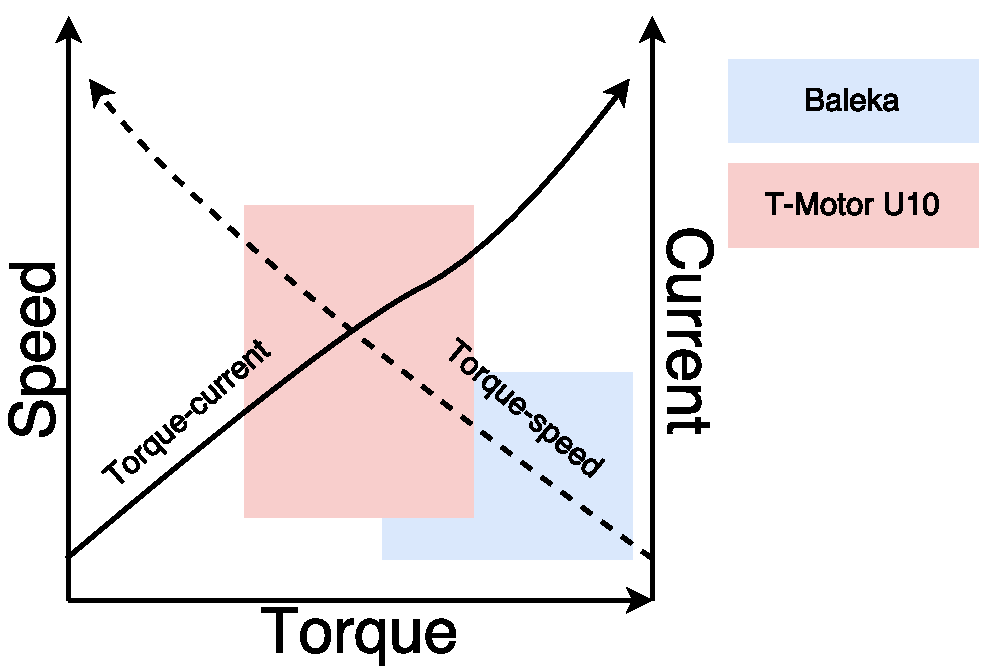
\includegraphics[width=0.6\textwidth]{images/motor/bldc-torque-speed-relation.pdf} 
\caption{Motor performance requirements.}
\label{fig:Motor performance requirements}
\end{figure}

\begin{figure}
\centering
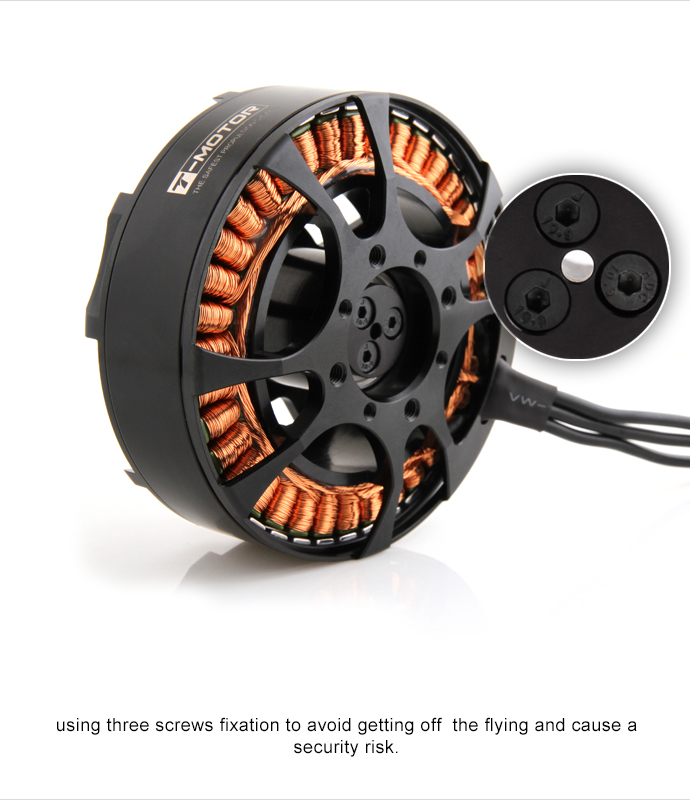
\includegraphics[clip, trim=0cm 5cm 0cm 2cm, width=0.4\textwidth]{images/motor/TMotorU10Plus} 
\caption{T-Motor U10 Plus Brushless DC Motor.}
\label{fig:TMotorU10Plus}
\end{figure}

\subsection{Motor Model Calculations}
\label{sec:Motor Model Calculations}

\subsubsection{Experimental Calculation of $K_t$ and $K_e$}
\label{sec:Experimental Calculation of Kt}

The motor torque constant, $K_t$, was calculated using the torque current relation $\tau = K_tI$. The leg was modelled as a virtual spring-damper system, as seen in \cref{fig:Leg spring-damper virtual model}. 

The spring constant, $K_{s1}$, was set to $200\ [N/m]$, and the damping and torsional spring-damping constants were set to zero. $K_t$ was tuned until the theoretical foot force matched the practical foot force measured via a load cell. The leg was fixed at a set height imposing a radial offset on the virtual spring-damper system.

For a spring constant of $200\ [N/m]$ and a radial offset of $0.15\ m$ a theoretical foot force of $K_{s1}\Delta r = 30\ N$ was expected. A mass of approximately $3\ kg$ was measured with $K_t = 0.08\ [Nm/A]$ set in the virtual leg model controller, resulting in a foot force of $3\ kg \times 9.81\ m/s^2 = 29.43\ [N]$. 

The study in \cite{Kalouche2016}, using the same T-Motor U10 Plus motors, calculated a torque constant of $K_t =  0.072\ [Nm/A]$. This confirms the experimental results obtained above.

For an ideal motor at a constant operating point, $K_e$ will equal $K_t$, as shown in \cref{eqn:ktke}.

\begin{equation} \label{eqn:ktke}
\begin{aligned}
&V_t = K_e\omega_m + IR_m \\
&\tau_m = K_t I \\
&P_{elec.} = V_t I = K_e \omega_m I + I^2 R \\ 
&P_{mech.} = \tau_m \omega_m = K_t I \omega_m \\
&P_{loss.} = I^2 R_m \\
&P_{elec.} = P_{mech.} + P_{loss.} \\
&\therefore K_e\ [V/rad/s]= K_t\ [Nm/A] = 0.08
\end{aligned} 
\end{equation}

Further force calibration and fidelity tests were performed in \cref{sec:Force Control Calibration and Fidelity}.

\subsubsection{Calculation of $R_m$ and $L_m$}
The resistance and inductance of the 3 phase windings of the motor were calculated using a lab multimeter to be $R_m = 47.5\ m\Omega$ and $L_m = 35\ \mu H$ respectively. 

Brushless DC motor windings are usually connected in WYE formation, as seen in \cref{fig:bldc-wye-connection}. This means the measured values for resistance and inductance were line-to-line values and had to be divided by two to get the per phase values above.

\begin{figure}
\centering
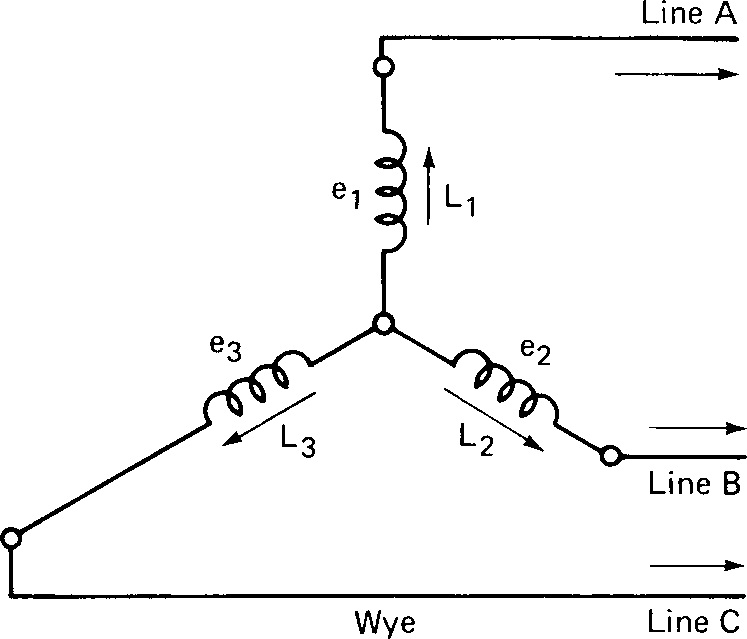
\includegraphics[width=0.4\textwidth]{images/motor/wye.jpg} 
\caption{WYE connected BLDC motor windings.}
\label{fig:bldc-wye-connection}
\end{figure}

\subsubsection{Calculation of $J_m$}
In order to calculate the moment of inertia of the motor, $J_m$, the ratio of acceleration torque to acceleration to steady state needs to be found. By commanding a DC equivalent current input of $1\ A$ and measuring the time taken to reach a steady state velocity, \cref{eqn:Jm} can be used to calculate $J_m$. The velocity vs. time plot used can be seen in \cref{fig:jm-plots}.

\begin{equation} \label{eqn:Jm}
\begin{aligned}
J_m &= \frac{T_{acc.}[N/m]}{a[m/s^2]} \\
&= \frac{IK_t}{a} \\
&= \frac{IK_t}{\frac{\Delta v}{\Delta t}}\ [kg/m^2]
\end{aligned}
\end{equation}

where $I=1\ A$, $K_t=0.08\ Nm/A$, $\Delta v = 1313.906\times \frac{2\pi}{60}\ rad/s$ and $\Delta t = 588.889\times10^{-3}\ s$.

This results in a motor moment of inertia of $J_m = 3.424 \times 10^{-4}\ [kg/m^2]$.

\subsubsection{Calculation of $B_m$}

The motor damping or viscous friction, $B_m$, was assumed to be negligible. Brushless DC motors have near zero damping and will have little effect on the simulated motor model.

\begin{figure}
\centering
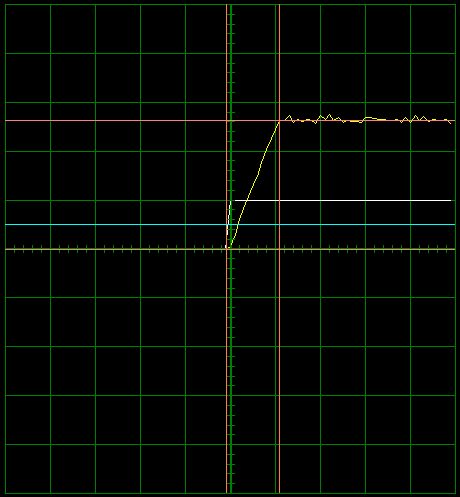
\includegraphics[width=0.5\textwidth]{images/driveware/current-velocity-response} 
\caption{Velocity vs. time plot for 1A equivalent DC command.\\
(500 rpm; 500 ms/div)}
\label{fig:jm-plots}
\end{figure}

\subsubsection{Calculation of $\tau_e$ and $\tau_m$}
The electrical and mechanical time constants of the motor, $\tau_e$ and $\tau_m$ respectively, can be used to plot a root-locus plot with poles at $-\tau_e$ and $-\tau_m$ as can be seen in \cref{fig:ol-motor-rlocus}. This is useful when designing a current controller for the system. $\tau_e$ and $\tau_m$ can be calculated using \cref{eqn:motor-time-constants}.

\begin{equation} \label{eqn:motor-time-constants}
\begin{aligned}
&K_m = \frac{1}{B_m} \\
&\tau_m = \frac{J_m}{B_m} \\
&K_e = \frac{1}{R_m} \\
&\tau_e = \frac{L_m}{R_m} 
\end{aligned}
\end{equation}

From \cref{eqn:motor-time-constants} and using the previously calculated motor constants, $\tau_e = 7.368 \times 10^{-4}$ and $\tau_m = 3.424 \times 10^{-4}$. This is assuming the motor viscous friction $B_m$ is insignificant which is usually the case in mechanically well made BLDC motors.

The resulting motor model open loop root-locus plot can be seen in \cref{fig:ol-motor-rlocus}. As expected the system has only negative real roots and will be stable in open loop.

\begin{figure}
\centering
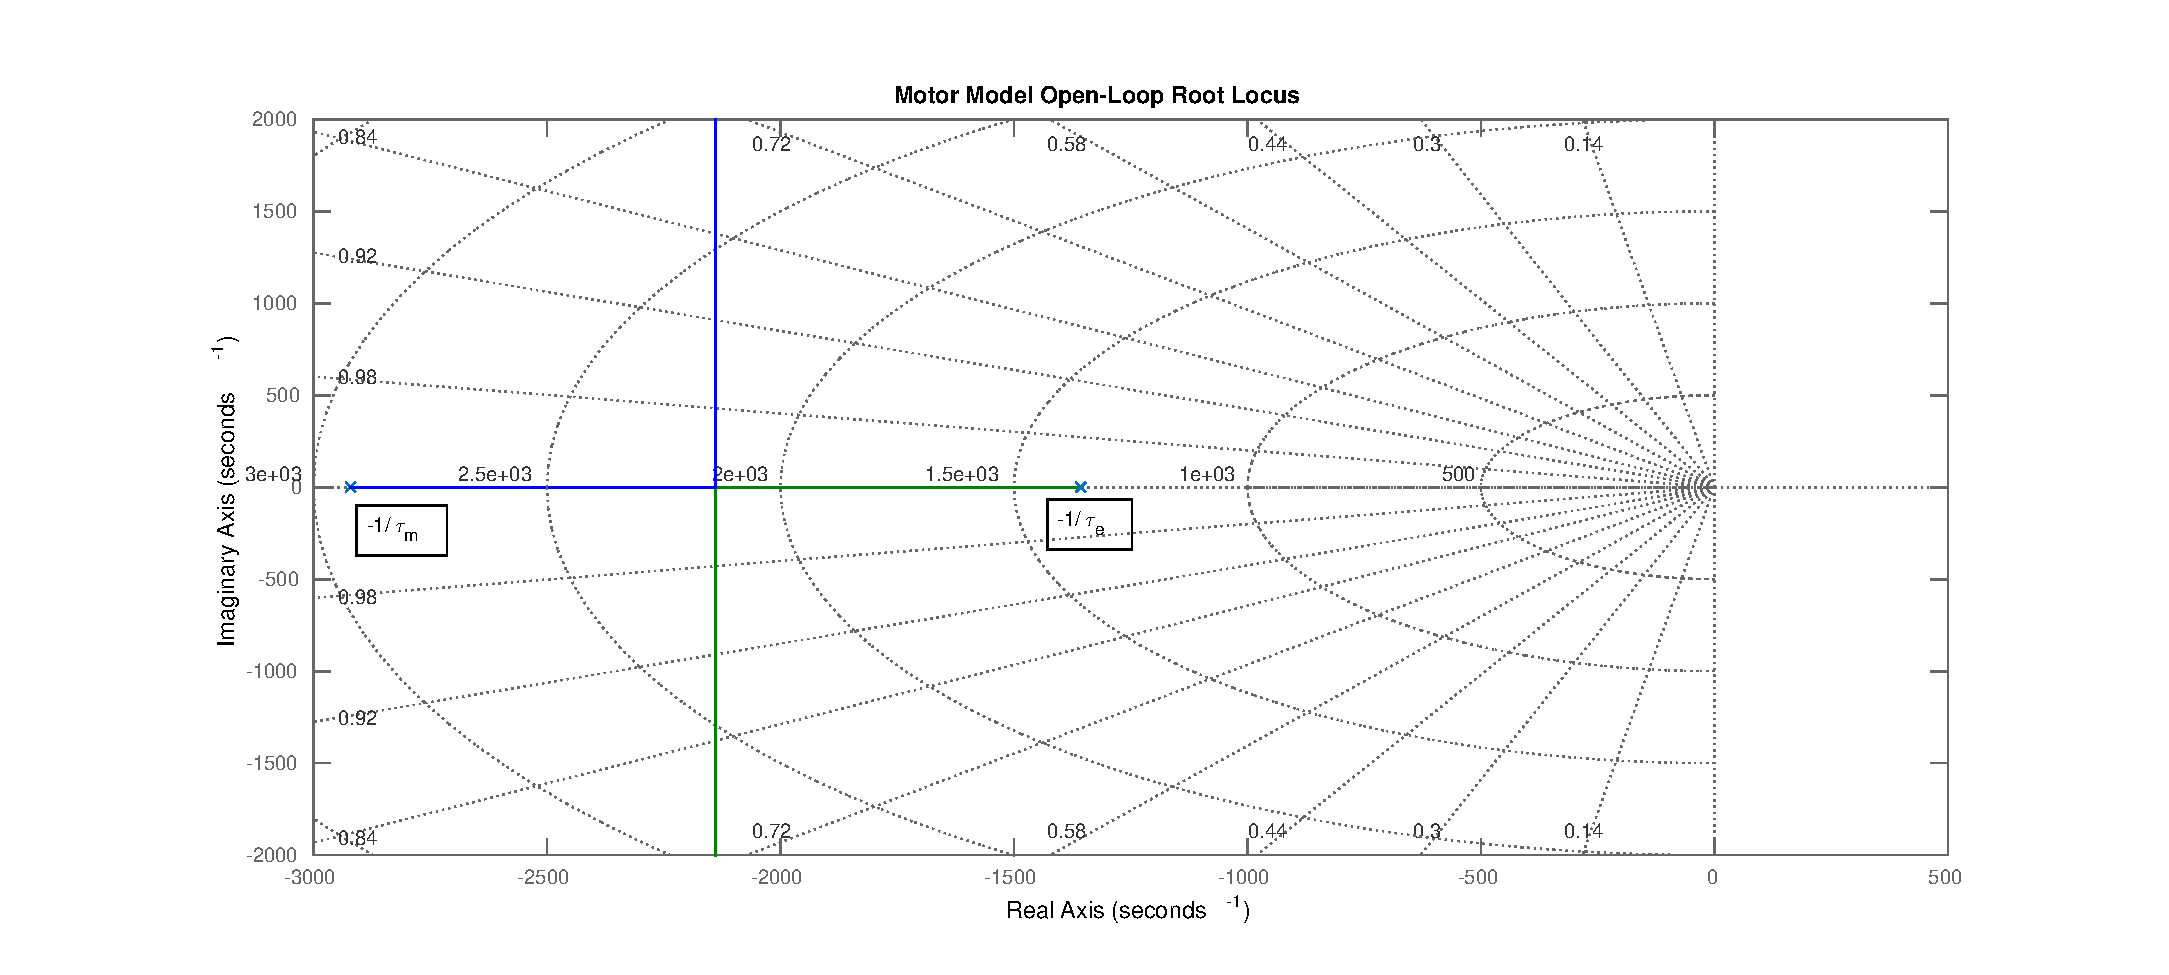
\includegraphics[width=1\textwidth]{images/motor/ol-motor-rlocus} 
\caption{Motor model open loop root-locus plot.}
\label{fig:ol-motor-rlocus}
\end{figure}


\subsection{Driver Configuration}
\label{sec:Driver Configuration}

The AMC drivers allow extensive customisation. After the motor, encoder, and general communication control parameters are configured, the PID control loops of the drivers can be configured, as seen in \cref{fig:AMCControlLoops}.

The motor drivers were initially configured with both on-board PID current and position control loops enabled. This allowed initial modelling of the motors, configuring of the motor encoders, and determining of the position limits (in counts). For control of the leg, the position control loop was finally implemented on the STM32F4 microcontroller, while using the existing current control loop of the motor drivers. The custom position control loop was indirectly implemented using the spring-damper virtual model and force control by setting the polar coordinate set-points, in comparison to the AMC driver position loop which used a PID controller specifically controlling position.

The AMC drivers were configured using the AMC Driveware configuration software, which provided an oscilloscope to measure the relevant motor responses as seen in \cref{fig:jm-plots,,fig:current-tuning-plots,,fig:position-tuning-plots}.

\begin{figure}
\centering
\includegraphics[clip, trim=2cm 5cm 2cm 8cm, page = 114, width=1\textwidth]{pdfs/AMC_DriveWareSoftwareManual.pdf} 
\caption{AMC DigiFlex Performance Servo Drive control loops (AMC, 2014).}
\label{fig:AMCControlLoops}
\end{figure}

\subsubsection{Current Control Loop}

By using a 1 A 120Hz square wave current command the current PI control loop was tuned, as seen in \cref{fig:current-tuning-plots}. Initially both  the proportional gain, $K_p$, and the integral gain, $K_i$, were set to zero. $K_p$ was slowly increased until the final amplitude of the current output just started to overshoot. $K_i$ was then set to minimize the steady state error. 

Values of $K_p = 0.277$ and $K_i = 0.262$ were obtained. Both motors were found to operate optimally with the same PI gain values.

\begin{figure}
\centering
\subfloat[][Motor driver current loop pre-tuning.\\ 
(200 mA; 5 ms/div)]{
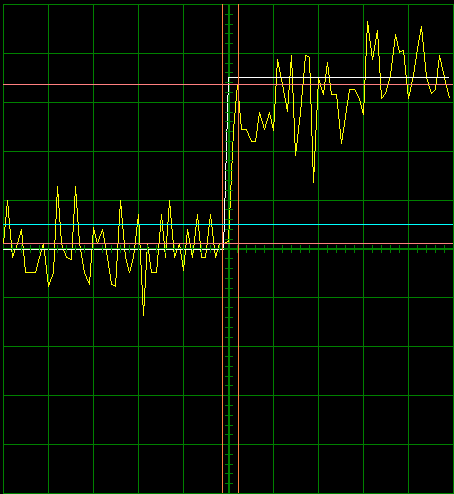
\includegraphics[width=0.4\textwidth]{images/driveware/current-pre-tuning-plot.png} 
}
\subfloat[][Motor driver current loop tuning - 1A 120Hz square wave command.\\(1 A; 1 ms/div)]{
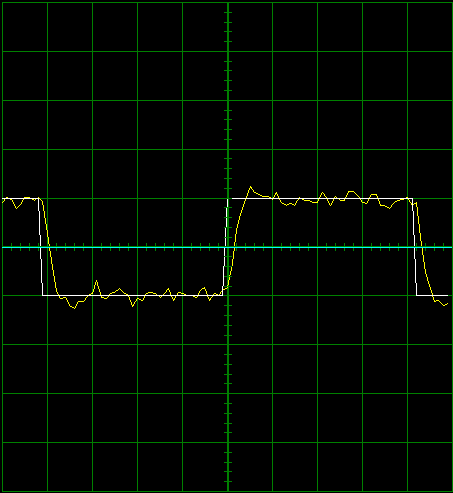
\includegraphics[width=0.4\textwidth]{images/driveware/current-tuning-plot.png} 
}
\caption{Motor driver current loop tuning plots.}
\label{fig:current-tuning-plots}
\end{figure}

\subsubsection{Position Control Loop}
The on-board AMC motor driver control loop was set up to test the encoder configuration. The encoder and relevant position limits can be seen in \cref{sec:motor-encoders}. 

A 1Hz sinusoid was used to tune the PID control loop gains. Values of $K_p = 0.0005793$, $K_i = 0.0006052$ and $K_d = 2.769e^{-9}$ were found to achieve optimal set-point tracking as seen in \cref{fig:position-tuning-plots}. The sinusoidal set-point can be seen in white and the position feedback in yellow. A 10-30 ms lag time can be seen due to the inertial load. This lag time causes a dead-band which should be considered when implementing a controller. 

These tests were performed with the leg attached - the inertial load provided by the leg made PID control loop tuning possible, whereas without any inertial load the BLDC motors overshot their set-point.

\begin{figure}
\centering
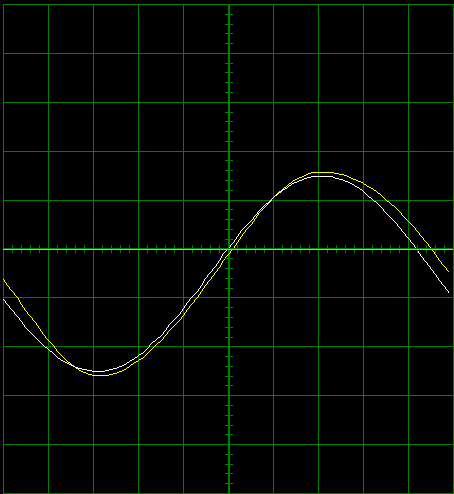
\includegraphics[width=0.4\textwidth]{images/driveware/position-tuning-plot} 
\caption{Motor driver position loop tuning - (-350:200) count 1Hz sinusoid command with 300 count offset.\\(100 ct; 100 ms/div)}
\label{fig:position-tuning-plots}
\end{figure}

\subsection{Motor Encoders}
\label{sec:motor-encoders}

The Avago Technologies HEDL-5640-A13 rotary encoder was used for feedback of encoder position to the motor drivers which then calculate the motor position and velocity relative to a starting encoder count position. 

The encoder has the following specifications:
\begin{itemize}
\item Optical sensing.
\item Incremental counting.
\item 500 counts per revolution.
\end{itemize}

The Avago encoder was chosen for its light, easily mountable frame along with the relatively high resolution position feedback of $0.72 deg./count$.
 
A shaft was designed to mount to the rear of the BLDC motor and interface to the encoder. The shaft was designed in OpenSCAD using programmatic CAD and can be seen in \cref{fig:encoder-shaft}. It was 3D printed by Justin Pead in White Lab using PLA plastic. 

The shaft was designed to be mounted using three hex screws to the provided mounting point on the rear of the motors. A star configuration was used for the interface between the shaft mounting point and the cylindrical encoder shaft so that these hex screws could be accessed easily.

Ideally the shaft should be milled using metal for better heat dissipation. Initially, before the aluminium mounting plate was used, the encoder shafts warped slightly while in operation and had to be bent back into shape. 3D printing was used for rapid prototyping and due to cost considerations.

\begin{figure}
\centering
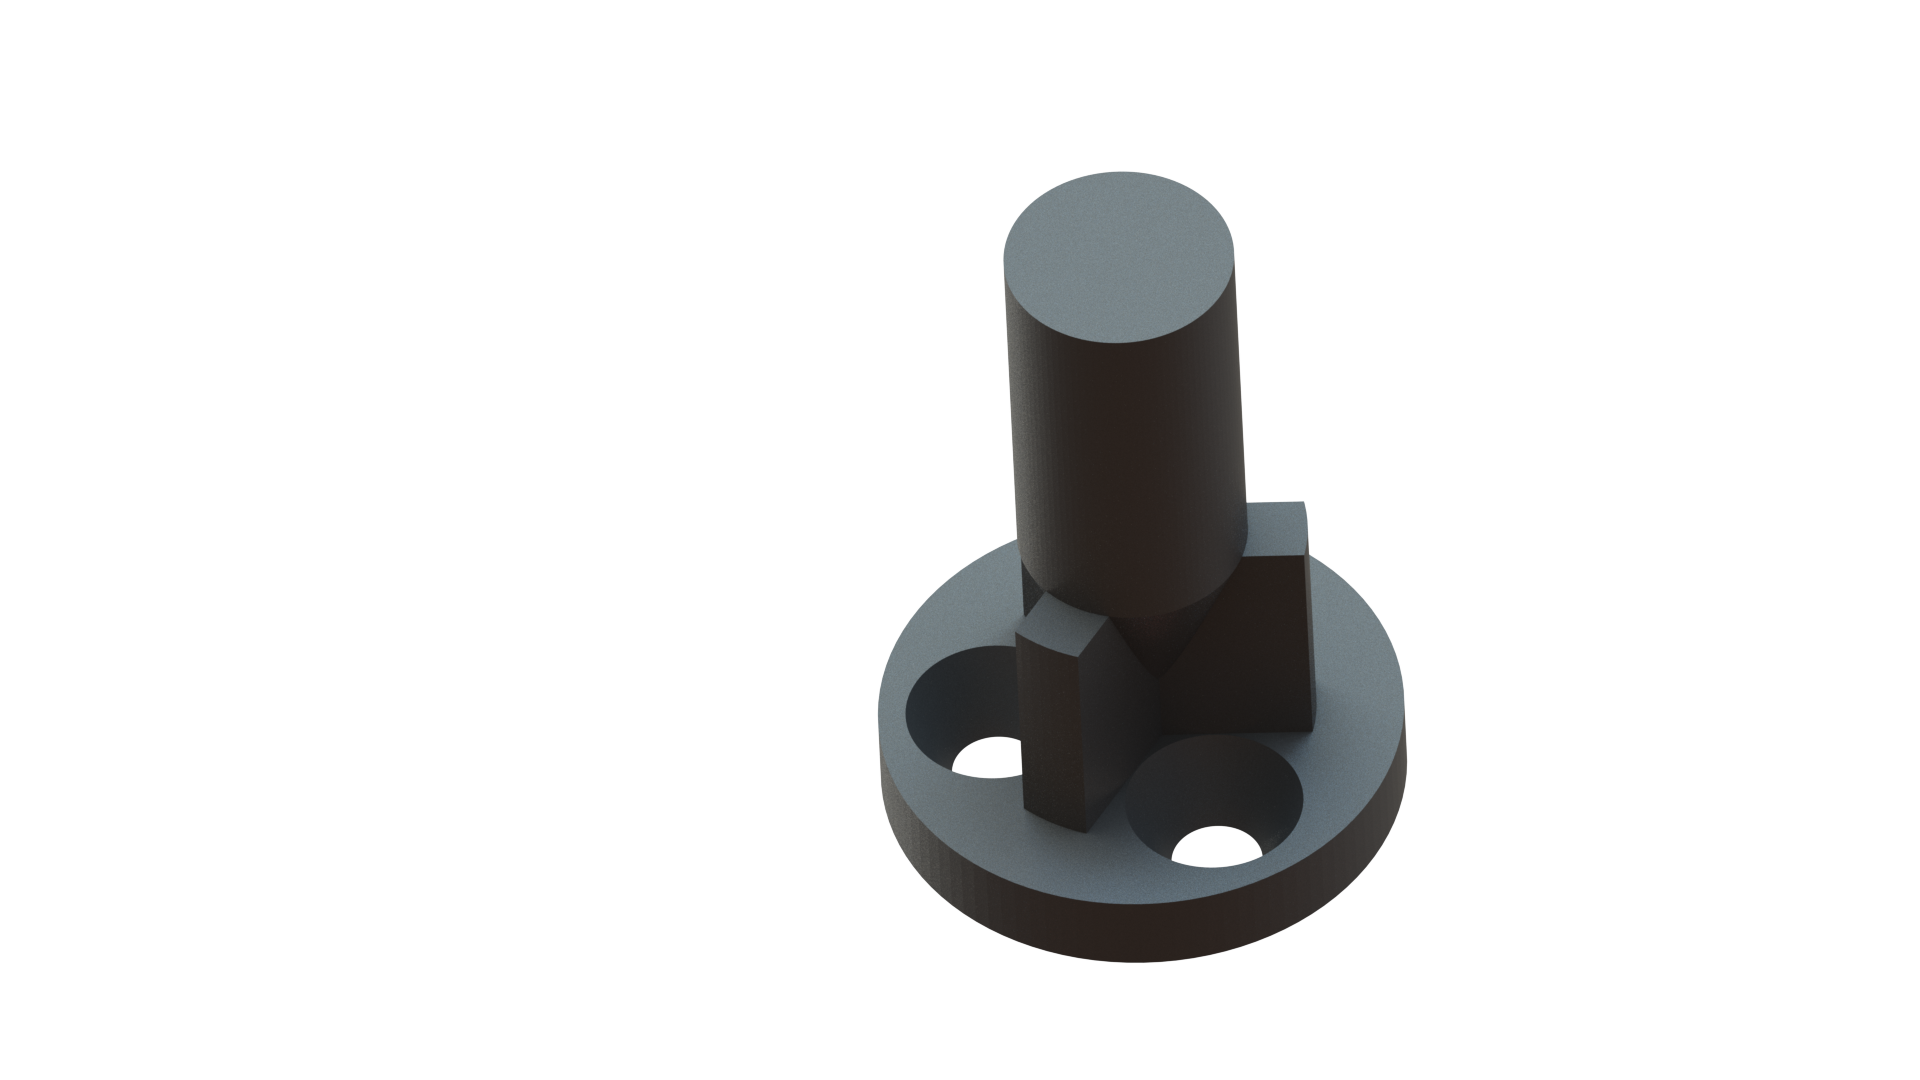
\includegraphics[clip, trim = 6cm 1cm 3cm 1cm, width=0.3\textwidth]{images/mechanical/encoder-shaft} 
\caption{3D printed PLA motor encoder shaft.}
\label{fig:encoder-shaft}
\end{figure} 

\definecolor{smokyblack}{rgb}{0.06, 0.05, 0.03}
\chapter{Software Development}
\label{chap:Software Development}

The development of two core project deliverables will be discussed:

\begin{enumerate}
\item Functional configuration, control and logging platform.
\item Reliable embedded system control system and motor driver communication protocol. 
\end{enumerate}

The following software development environments were considered: C/C++ (Qt), Python, Processing (dedicated graphic programming), and Matlab (serial toolbox). 

The Qt C/C++ GUI development environment was chosen for the following primary reasons:

\begin{itemize}
\item Low over-head programming language.
\item Open source software.
\item Low level computer hardware access results in near real-time serial packet processing and accurate timing.
\item Compatibility with C packed struct packet encoding and decoding code (as developed in \cref{sec:Packet Transmission}).
\end{itemize}

The design, operation and commissioning of the software system will be covered in detail. 

\section{RTOS Communication Protocol}

Ideally FreeRTOS tasks should operate with as much isolation as possible, with each task performing a specific function with different priority levels. In the case of a communication protocol, the overall task is inherently sequential so this leads to FreeRTOS being used in a sequential way with all tasks operating at real-time priority level. 

FreeRTOS was chosen because of the following benefits:

\begin{enumerate}
\item Segmentation of code into specific tasks provides readable code for future users.
\item FreeRTOS task configuration provides a framework for future embedded robotic control systems as well as easily reconfigurable code.
\item Semaphores and queues lend themselves to sequential reception and processing of packets at predefined intervals very well.
\item Isolation of tasks provides easy debugging of communication issues.
\end{enumerate}

\subsection{Heartbeat Task}
The \textit{Heartbeat} task's primary function is to synchronise the communication protocol. It is the only task running with a 5 ms non-blocking delay. Every 5 ms it completes the following functions:

\begin{enumerate}
\item Compiles a read command packet for current, position and velocity.
\item Appends these three packets to the two motor driver transmit queues. 
\item Gives a binary semaphore to the motor 1 and motor 2 transmit tasks.
\item Starts a 5 ms non-blocking delay to allow the two motor transmit tasks to complete their transmission and for the motor driver replies to be received and decoded.
\item Gives a binary semaphore to the PC transmit task to compile and send the newly received motor data for logging.
\end{enumerate}

\subsection{PC TX Task}
The \textit{TXPC} task is used purely for logging of data over serial on the Baleka C++ application, as seen in \cref{chap:Graphic User Interface}. 

Data is received in a queue from both the motor \textit{RXMotor1} and \textit{RXMotor2} tasks as well as the \textit{Controller} task which is compiled into a packet along with status bits indicating various events and conditions. 

Status bits in the packet indicate to the PC logging software whether specific data has been successfully received by the \textit{PCTX} task in the queue. A CRC check is added for transmission based error detection. 

The task is run every $5\ ms$ once the motor data has been requested, received and processed, and the \textit{Controller} task has instructed the motor drivers to perform a specific command. 

\subsection{PC RX Task}
The \textit{RXPC} task is the only task that is required to perform non-synchronous reception of packets. The DMA reception is initialised and then the task waits until the full PC packet has been received. The RX complete interrupt handler then gives the \textit{PCRX} task a semaphore to continue decoding of the data. The use of non-blocking DMA UART reception and semaphores ensures other tasks are able to run during the reception process.

The \textit{RXPC} task checks how much data has been received before searching for the start-bytes of the packet. Once a valid packet has been found it is copied to a packed struct  and the CRC is calculated and compared to the CRC member of the struct. If it is valid then the \textit{RX\_DATA\_VALID} flag is set, this indicates to other tasks that they can safely use the packet data received. 

Every packet has an op-code that indicates what data is present in the packet. A switch statement is used to process the data appropriately and perform the necessary functions. These functions range from configuring the motor drivers, killing the drivers, calibrating motor positions and triggering various on-board events such as jumping and leg trajectories. All these functions operate by setting flags or compiling packets to be sent to the necessary queues for transmission.

An example of the packet processing code can be seen in \cref{listing:PC RX packet processing}.

\subsection{TX Motor Task}
The \textit{TXMotor} task functions as an interface between the rest of the tasks and the motor driver. The task is periodically run when a semaphore is received.

When the task starts a DMA reception from the motor drivers is initialised, which will only be halted once control is handed over to the \textit{RXMotor} task. 

Every time the task runs, at least three command packets are sent to the motor driver from the \textit{TransmitMQ} queue. This queue is filled by the \textit{Heartbeat} task which synchronises all communication protocol tasks. The three command packets request current, position, and velocity data from the motor drivers which is processed by the \textit{RXMotor} task and used in the control loop every $5\ ms$. 

The queue runs in a loop until transmission is complete, with a number of timing conditions being completed to ensure that a reply is received from the motor driver before the next request is transmitted - if this is not done properly then data can be lost. 

The other three queues are used for current commands, position commands, and for general motor driver management commands such as changing gain sets or initialising the motors. An important task for the general driver management queue, \textit{CommandMQueue}, is to disable the motor drivers when position and/or current limits are reached.

\subsection{RX Motor Task}
The \textit{RXMotor} task is used to process data received from the motor driver in a reply to a command. The task waits to receive a semaphore from the \textit{TXMotor} task, after which the DMA reception is halted. 

The task then begins processing the data by:

\begin{enumerate}
\item checking how much data has been received,
\item  searching the buffer and finding the index of all start bytes,
\item finding unique user programmable op-codes based on location of start bytes,
\item using a switch statement to appropriately decode data using a packed struct based on the op-code,
\item and adding this data to a buffer before moving on to the next start byte index for processing.
\end{enumerate}

This data buffer is then sent to the \textit{Controller} and \textit{TXPC} task queue before waiting for a semaphore to be received again.

\subsection{Controller Task}

The controller task's core function is to reliably implement the control loop design seen in \cref{fig:virtual-model-impedance-loop} and developed in \cref{chap:Controller Development}. This means the controller task runs at a consistent $200\ Hz$ frequency.

The control loop waits for new data to be received from each motor on a queue from the \textit{RXMotor} task - this is expected to happen every $5\ ms$. If an error occurs or the data received from the drivers is invalid then the control loop will not run for safety. 

Once the data has been received, if a valid \textit{RXPC} packet is available it is checked for virtual model configuration data which is then used to set up the spring-damper model.

A \textit{TRIGGER} flag and \textit{START} flag are both checked before functions are run or the controller is allowed to operate. The \textit{TRIGGER} flag is used to start jump and trajectory sequences.

Multiple calculations are performed to implement a control model:

\begin{enumerate}
\item Cumulative integral error term.
\item Jacobian mapping for velocity and position.
\item Spring-damper force vector which is mapped using to motor torques using Jacobian.
\item Torque current command mapping using torque constant as derived in \cref{sec:Motor Model Calculations}.
\end{enumerate}

If there are invalid kinematic or current set-points a kill function is implemented that both stops the control loop from operating and kills the motor driver bridge.

If a current command is successfully calculated, a motor driver command is compiled and sent to the \textit{TXMotor} task queue.

\subsection{FreeRTOS Timing}

The default 1000 Hz tick rate was overridden with a tick rate of 5000 Hz to enable more fine tuned packet timing and delays. The timing configuration can be seen in \cref{listing:FreeRTOS timing}. 

In order to achieve a control loop rate of 200 Hz, a sampling time of 5 ms or 25 ticks was used.

\begin{figure}
\centering
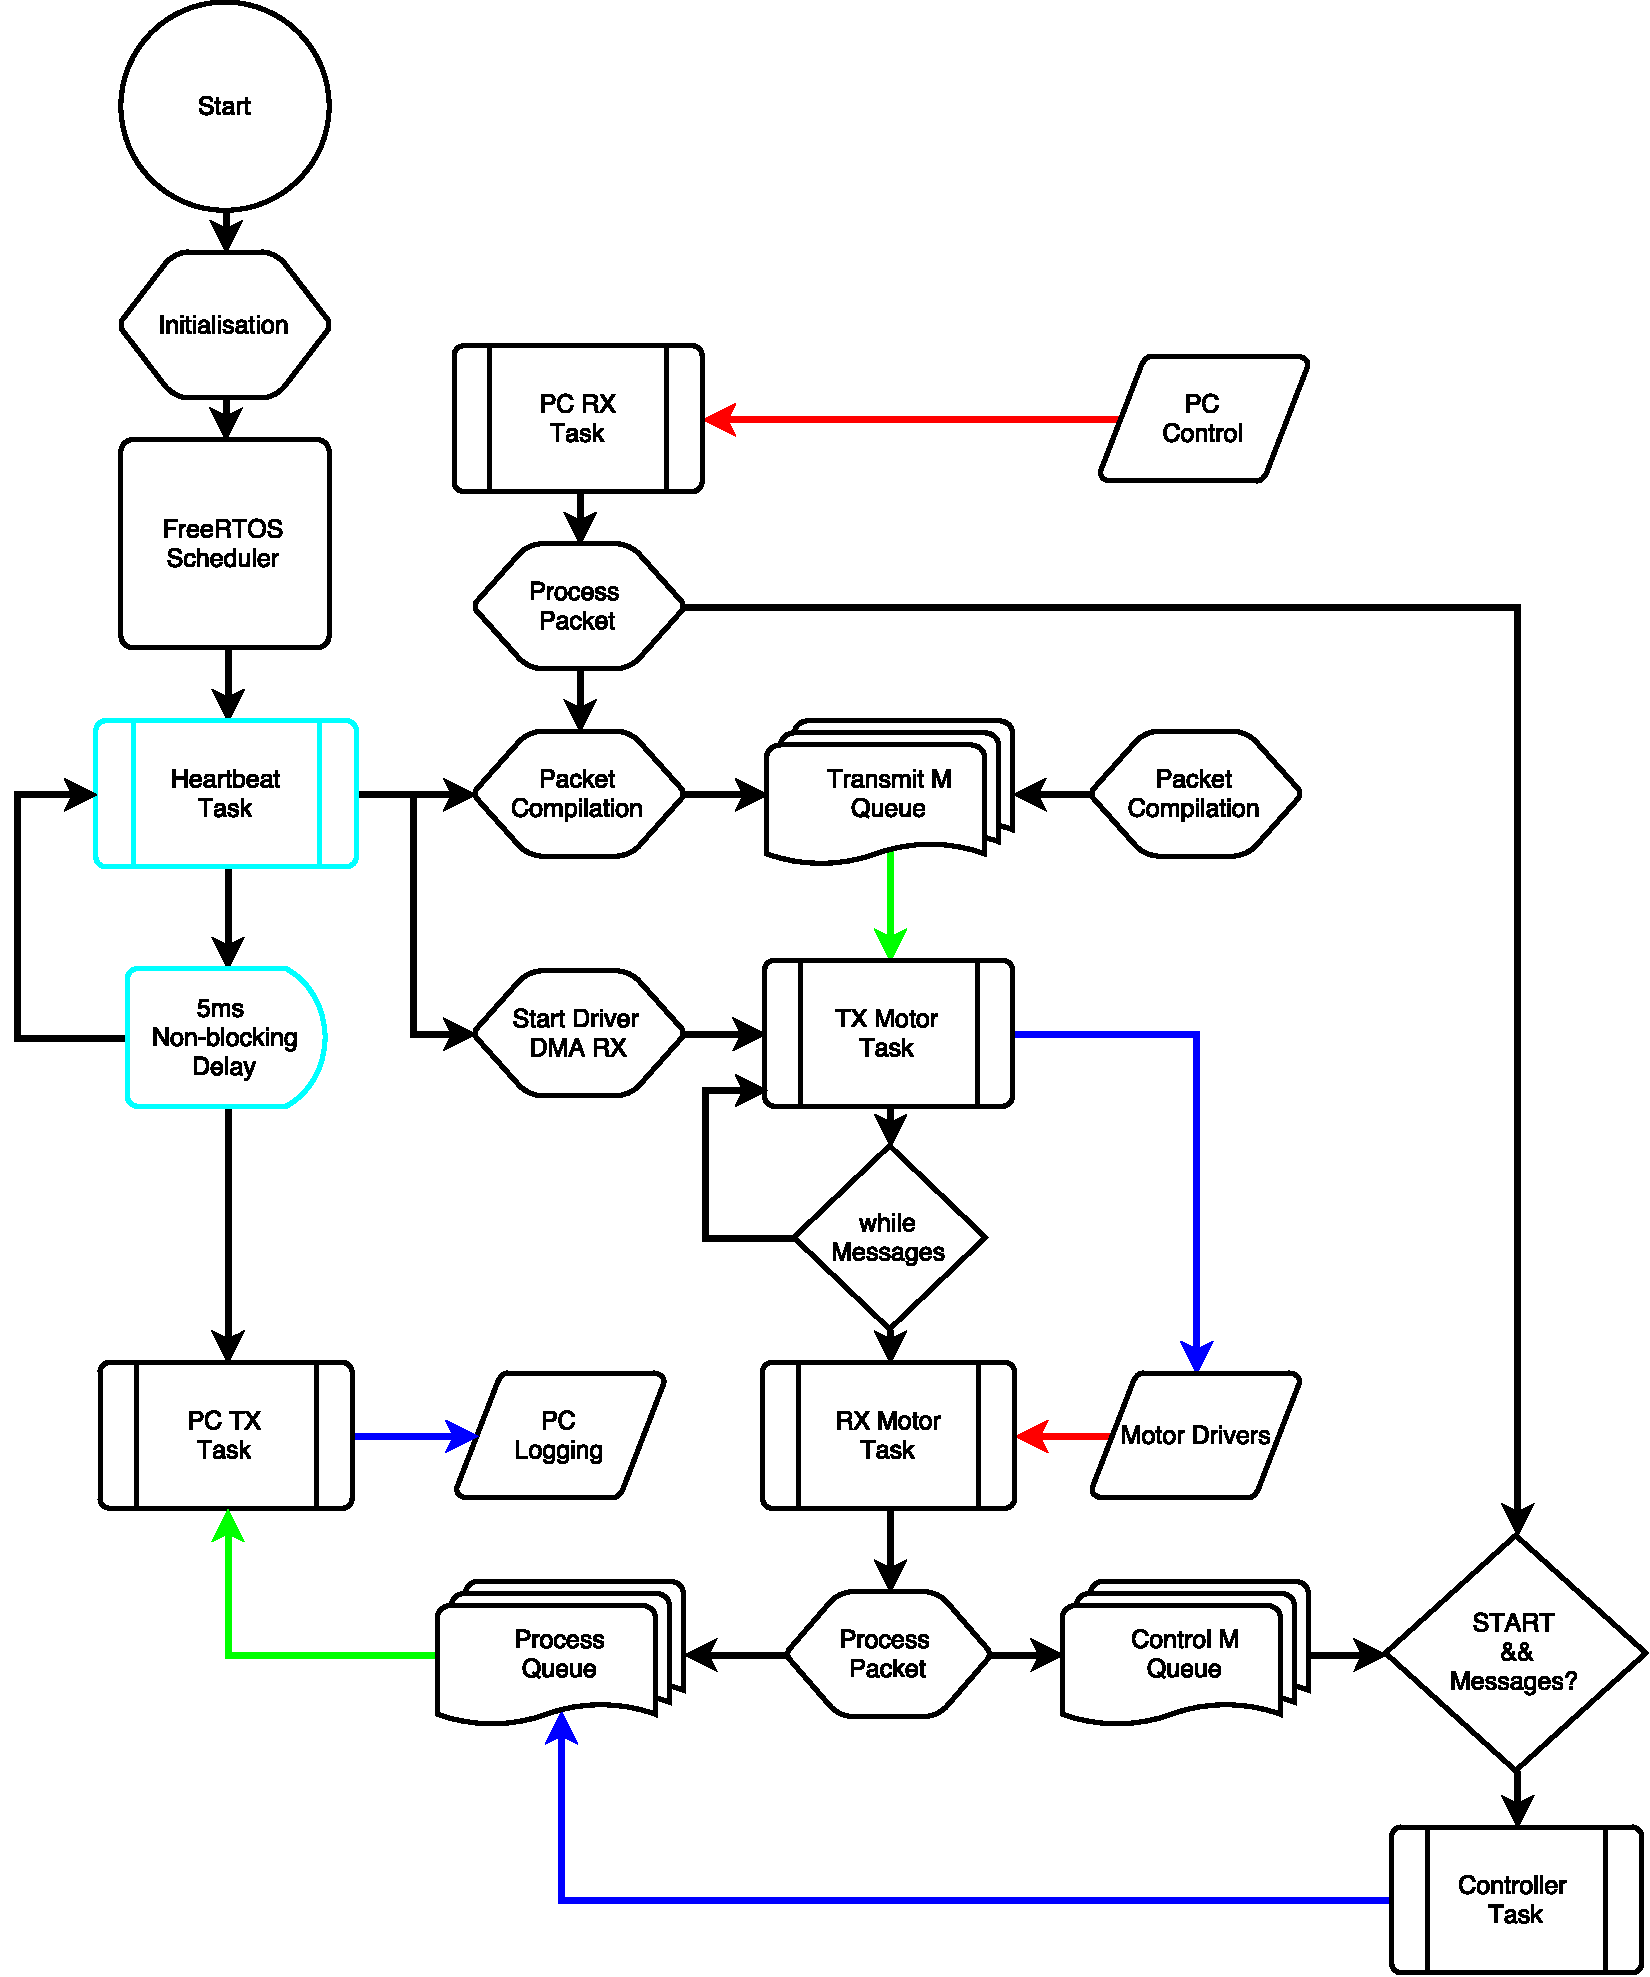
\includegraphics[width=1\textwidth]{images/comms/communication-flow-diagram.pdf} 
\caption{FreeRTOS communication protocol flow diagram.}
\label{fig:FreeRTOS communication protocol flow diagram.}
\end{figure}

\section{Packet Transmission}
\label{sec:Packet Transmission}

\subsection{Structuring}
\label{sec:structuring}

Usually when a C compiler stores data in memory it does so in a manner that optimizes memory access speed. In the case of a struct this isn't intuitively in successive memory addresses, but with padding.

Packets are compiled and transferred in bytes, the smallest variable size on any architecture apart from bit fields. A simple and elegant solution to packet structuring and decoding is to use a struct where the individual bytes are consecutive and byte aligned, much like an array, but with the benefit of accessing by struct member too.

This method has a few major benefits:
\begin{itemize}
\item To decode packets the data can be copied from a receive buffer directly over a struct and each of the struct members will contain the appropriate "decoded" data.
\item To structure and compile a packet, all the relevant data can be assigned to a struct member and then when the packet is ready to be transmitted it is as simple as passing a pointer to the first value of the struct along with the packet length.
\item The CRC check can be performed on a sequence of struct members with the guarantee that all members are consecutive and byte aligned.
\item The packet length is the size of the struct!
\end{itemize}

The way to ensure that bytes are consecutive and byte aligned is to use the $\_\_$attribute$\_\_$((packed)) C compiler type attribute. This is a compile time flag that forces the struct to be byte aligned with no padding. An example of a packed struct from the embedded software can be seen in \cref{listing:packed-packet} in \cref{app:Communication Protocol Code}.

\subsection{Integrity Checking}

A Cyclic Redundancy Check was implemented for all communication. Polynomial division is performed on the data contents of the packet, this results in a remainder that constitutes the CRC that is appended to the packet. If this CRC does not match the calculated CRC on the receiver side then measures are taken to deal with the corrupt packet. 

The CRC ensures the communication system is robust to interference and corruption, which can come from a number of sources:

\begin{itemize}
\item 3 phase alternating current flowing through motor phase wires.
\item Motor EMF generated.
\item RTOS and embedded system errors due to synchronisation.
\end{itemize}

Two CRC protocols were used. The CRC calculation function developed by James Gowans in December 2012 was customized to work with the motor driver two byte CRC protocol.

The iNemo and PC packets used the CRC-16/CCITT-FALSE protocol and the motor drivers are hard-coded to use the XMODEM protocol, with the configuration seen in \cref{tbl:CRC protocol configuration} and originally found in \cite{gregcook2016}.

In order to reduce CPU time used for CRC calculations, two CRC lookup tables are generated before the RTOS scheduler takes control.

\begin{table}[]
\centerline{
\begin{tabular}{lllllllll}
\textbf{Device}       & \textbf{Protocol} & \textbf{Width} & \textbf{Polynomial} & \textbf{Init} & \textbf{Refin} & \textbf{Refout} & \textbf{XORout} & \textbf{Check} \\
\textbf{iNemo/PC}     & CCITT-FALSE       & 16             & 0x1021              & 0xffff        & FALSE          & FALSE           & 0x0000          & 0x29b1         \\
\textbf{Motor Driver} & XMODEM            & 16             & 0x1021              & 0x0000        & FALSE          & FALSE           & 0x0000          & 0x31c3        
\end{tabular}
}
\caption{CRC protocol configuration.}
\label{tbl:CRC protocol configuration}
\end{table}

\subsection{Compilation}

\subsubsection{Motor Driver Packet}

A function was created to compile motor driver command packets based on the AMC motor driver packet protocol. The \textit{BaseCommandCompile} function prototype can be seen in \cref{listing:Motor packet compilation function}. 

All motor driver packets either request data from a memory address or contain data to be written to a memory address. The command bits \textit{ComBits} of the function are written to the packet, where 0x02 tells the motor driver to set data and 0x01 tells the motor driver to read data. \textit{INDOFF1} and \textit{INDOFF2} indicate the motor controller address and offset for reading or writing of data. 

The \textit{SeqBits} are a unique sequence of 4 bits that function as an ID for the packet - the motor driver will reply with the same ID to indicate which command it is responding to. The response sequence bits are then used as an op-code for the packet processing switch statement used in the \textit{RXMotor} RTOS task.

Some of the function inputs set up the structuring of the packets and identify the packets within the embedded system. \textit{DATA} is a pointer to the data to be written to the address, \textit{LEN} indicates how many bytes of data must be read from the motor driver address and \textit{SNIP} is a parameter that is a workaround for proper packet compilation indicating how many bytes must be removed from the packet if the packet is for requesting data rather than writing data.

The final function input, \textit{n}, is an index for the packet. This is an index for the array of structs that is used to compile the packets. This way when a packet command is to be sent to a function on one of the RTOS queues, just the index can be sent. 

An example of an array of structs can be seen in \cref{listing:Motor packet array of structs} and an example usage of the \textit{BaseCommandCompile} function can be seen in \cref{listing:Motor packet compilation example}.

All of the parameters, op-codes and other information relating to motor command packet encoding can be found in \cref{tbl:motor-driver-protocol} in \cref{chap:Motor Driver Command Protocol}.

\begin{listing}[]
\begin{minted}[
linenos,
bgcolor=smokyblack]{c}
void BaseCommandCompile(uint8_t n, uint8_t SeqBits, uint8_t ComBits, 
uint8_t INDOFF1, uint8_t INDOFF2, uint8_t *DATA, 
uint8_t LEN, uint8_t SNIP);
\end{minted}
\caption{Motor packet compilation function.}
\label{listing:Motor packet compilation function}
\end{listing}

\subsubsection{PC Packet}

The structure of the packets both received and transmitted by the PC can be seen in \cref{fig:pc-rx-packet} and \cref{fig:pc-tx-packet} respectively.

The typical start and stop byte (one) were replaced with start and stop bytes (two), being \textit{~[} and \textit{]~} respectively. This removed the need to search for and remove any start or stop byte in the packet data before transmitting. The chance of there being a series of two start or stop bytes in the data is $1$ in $16\times 16\times 16\times 16 = 65536$. 

In \cref{fig:packet-timing} the transmission duty cycle for packets transmitted from the embedded system to the PC, the larger of the two packets, is approximately $20 \%$ - this leaves plenty of time for additional data to be transmitted. The PC TX packet is 75 bytes and the PC RX packet is 59 bytes. As additional data is appended to the packets via the packed struct, the protocol allows for quickly reconfiguring transmission and reception processes to accommodate this extra data for logging and live plotting. 

The status bit field of the packet allows individual bits to be used as variables - this is a special C variable type that is useful for creating a sort of binary flag in the packet. 

The trigger bits of the \textit{PC TX} packet allows various events and sequences to be started in the embedded system control loop.

\begin{figure}
\centering
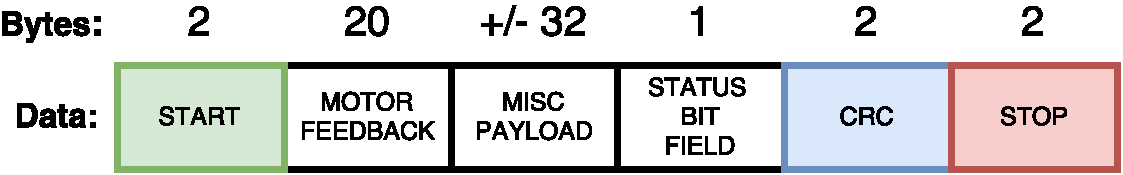
\includegraphics[clip, trim=0cm 0cm 0cm 0cm, page = 1, width=1\textwidth]{images/comms/pc-rx-packet.pdf} 
\caption{PC RX packet structure.}
\label{fig:pc-rx-packet}
\end{figure}

\begin{figure}
\centering
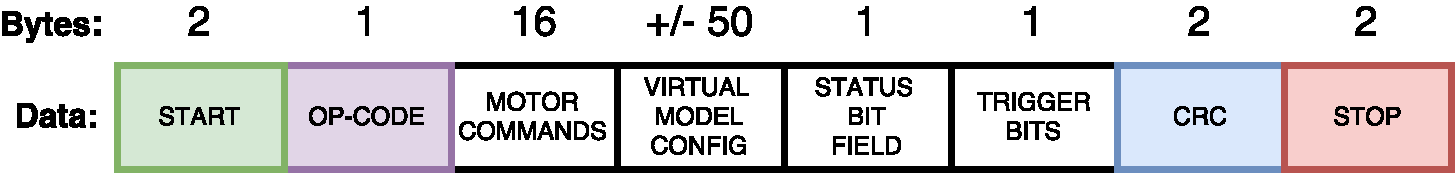
\includegraphics[clip, trim=0cm 0cm 0cm 0cm, page = 1, width=1\textwidth]{images/comms/pc-tx-packet.pdf} 
\caption{PC TX packet structure.}
\label{fig:pc-tx-packet}
\end{figure}

\section{Peripheral Configuration}

A basic peripheral configuration diagram can be seen in \cref{fig:microcontroller-peripheral-config} showing which UART and GPIO ports are routed to which pins.

\begin{figure}
\centering
\includegraphics[clip, trim=1cm 7cm 1cm 7cm, page = 2, width=0.8\textwidth]{pdfs/BalekaSTMConfig.pdf} 
\caption{STM32F4 microcontroller peripheral configuration.}
\label{fig:microcontroller-peripheral-config}
\end{figure}

\subsection{Protocol}

A number of serial protocols were used in the communication system. To reduce noise interference from motor EMI the RS-485 protocol was used. RS-485 uses differential signalling with a $200\ mV$ binary threshold. This protocol is designed for long distance low noise data transmission at data rates up to $10\ MBits/s$ at short to medium range. 

The VD30 and VD485 RS-485 driver ICs were used to couple the TTL serial logic of the microcontroller to the RS-485 transmission lines. A RS-485 to TTL serial USB converter was used to interface with the PC. The iNemo microcontroller was directly connected via TTL level serial to the microcontroller. The communication protocol configuration can be seen in \cref{fig:uart-communication}.

\begin{figure}
\centering
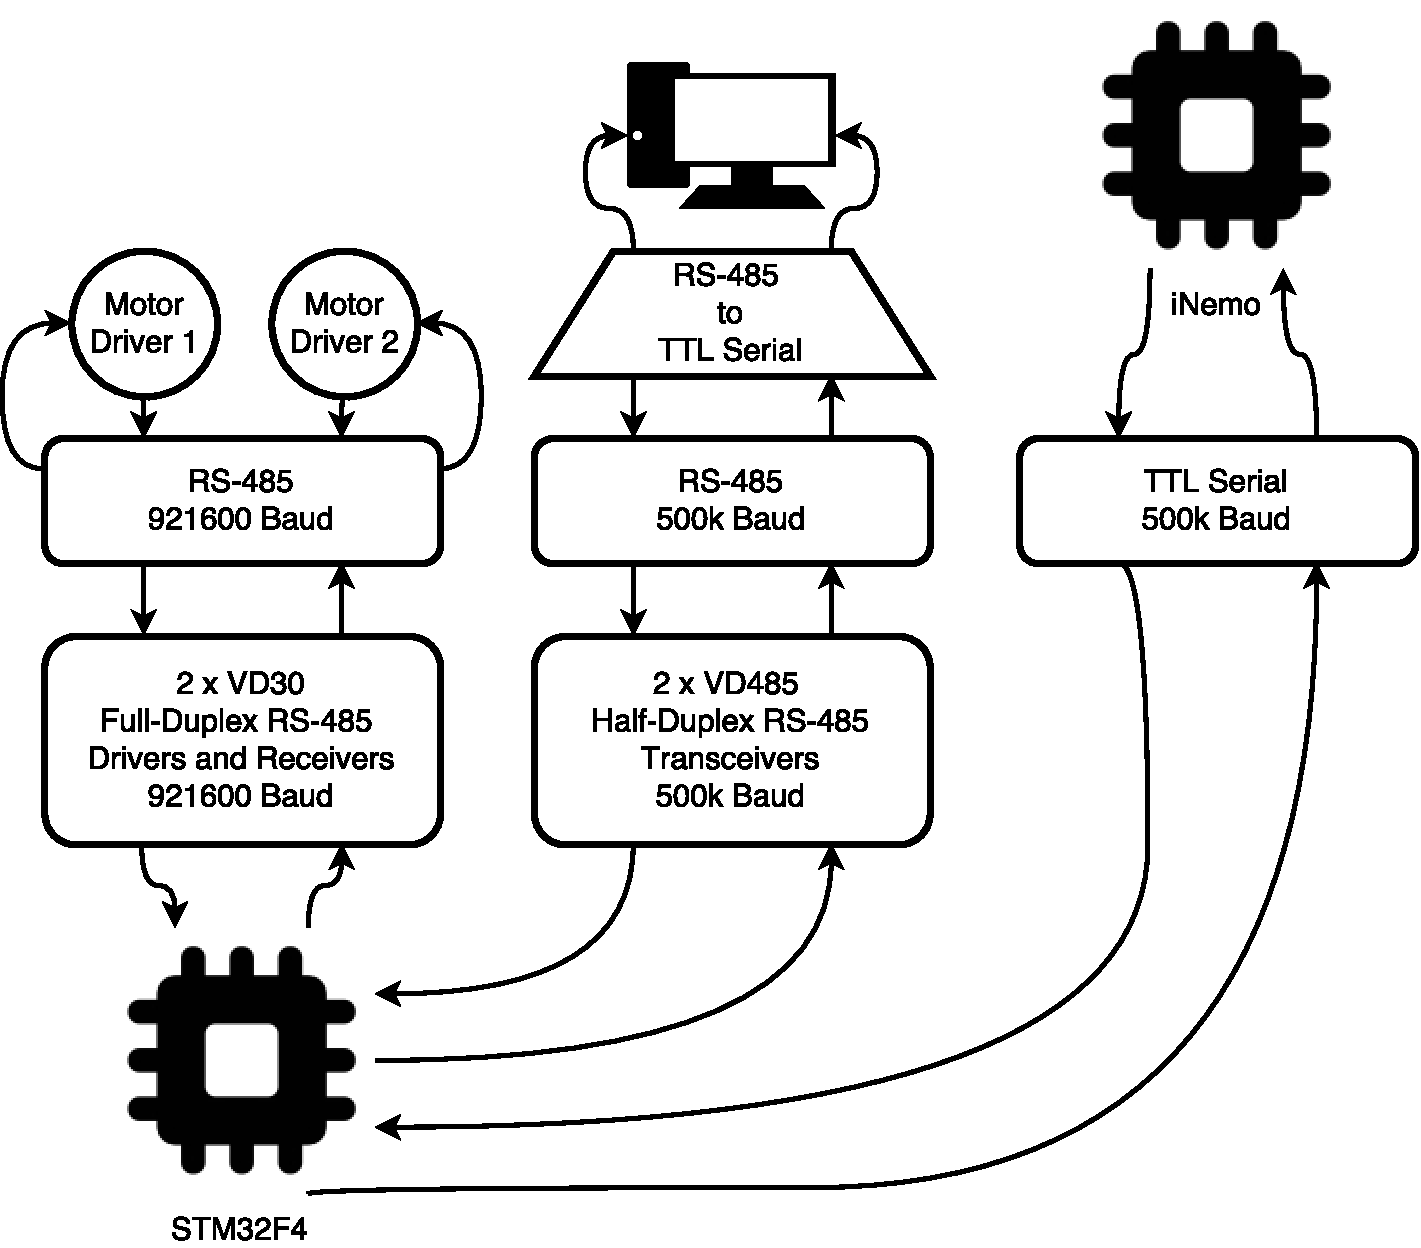
\includegraphics[width=0.8\textwidth]{images/comms/uart-communication.pdf} 
\caption{STM32F4 UART Serial Protocol.}
\label{fig:uart-communication}
\end{figure}

\subsection{Data Rates}

Two data rates were selected for the motor driver interface, and the iNemo and PC interface. 

The maximum communication speed of the motor controllers is 921600 baud over RS-485. Due to the high speed control loop frequency, and in order to achieve the high density packet transmission and reception as seen in \cref{fig:packet-timing}, the 921600 baud rate was selected.

In \cref{fig:packet-timing} the motor 1, M1, command and reply sequence can be seen. Every time a command is sent the corresponding reply has to be received before the next command can be sent. This is an on-board motor driver problem, when commands are sent before the previous reply the motor driver fails to perform the command. This bottle neck greatly reduced possible control loop frequency. Without this limit it would be possible to achieve upwards of $500\ Hz$ control loop frequencies resulting in much more accurate virtual model control.

The PC and iNemo data rate was limited to 500k baud for stability and noise rejection. The Qt application began to miss packets when the data rate was increased above 500k baud - this is likely due to the lack of DMA on personal computers and the overhead of the application. The iNemo was to be used for transmitting relatively small packets containing accelerometer and gyroscope data, so the data rate of 500k baud was adequate for this purpose.

If the need arises to append additional data to the communication packets the baud rate could be increased further to accommodate this within the $5\ ms$ maximum transmission period.

\subsection{Direct Memory Access}

DMA was used for all UART communication on-board the STM32F4. DMA enables control of the data transmission and reception process to be handed over to the DMA controller, of which there are two on board the STM with a number of streams. This means that rather than having an interrupt to process each received byte (10 bits in practise with the parity bit etc.), the memory is directly accessed by the DMA controller when transferring data from the receive buffer to a memory address which avoids using CPU time.  

\begin{figure}
\centering
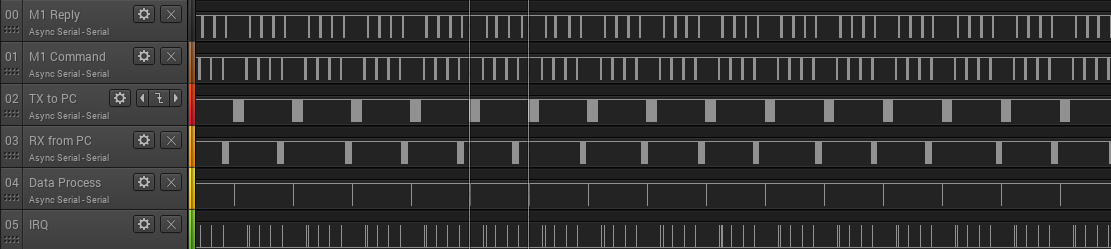
\includegraphics[width=1\textwidth]{images/comms/pc-packet-timing-data} 
\caption{Communication protocol packet timing with 5 ms sampling rate.}
\label{fig:packet-timing}
\end{figure}

\section{Graphic User Interface}
\label{chap:Graphic User Interface}

To enable rapid prototyping, a basic pre-existing serial logging platform was used and plug-ins were developed to adapt the software for controlling, configuring, logging and live plotting of the Baleka robotic leg platform. 

qSerialTerm, described as "A Qt based Serial Port terminal emulator", was built upon. It is distributed under the GNU General Public License (GPL) v3, which allows distribution, customisation and even sale of software published under the license, so long as basic conditions are met. It is copyright 2012 by Jorge Aparicio who's software repository can be found on GitHub: \url{https://github.com/JorgeAparicio/qSerialTerm}\cite{jorgeaparicio2013}.

Qt Creator CPP was used for the software development and can be compiled to run on both Linux and Windows platforms - for reference all development was completed on a Linux platform.

Three .cpp files were used for the majority of the added functionality, namely: CRC.c, framewidget.cpp and serialportwidget.cpp along with their respective header files and Qt forms.

\subsection{Serial Communication}
\label{sec:Serial Communication}

The serial interface is the first step in configuring UART communications. After successfully opening a port it allows you to select basic configuration options. The GUI extract can be seen in \cref{fig:serial-config}\cite{jorgeaparicio2013}.

A button was added, \textit{Default}, to allow quick set up of the software for experimentation with the Baleka leg. 

The maximum stable baud rate with the Qt software was 500k, any higher and the accuracy of the packet timing decreased due to application overhead. 

The refresh rate, when set to any value lower than $10\ ms$ tended to vary by as much as $5\ ms$ during operation. On Unix based operating systems the quoted accuracy of software timing is $\pm 1\ ms$ and for Windows machines it is $\pm 5\ ms$, making the decision to use a Linux machine natural. The Qt software timer resolution was increased to allow the possibility of a $200\ Hz$ refresh rate. 

The refresh rate was used to set the packet reception and transmission frequency. Due to the inconsistent timing real-time control of the leg from the Qt application was not possible, this was because of the large $\pm 60$ byte packets being transferred and the application overhead.

A compromise was found by using the Qt application for configuration of the virtual model and performing non-time critical tasks, as well as real-time logging, while the real-time control was implemented on the STM32F4 embedded system.

\begin{figure}
\centering
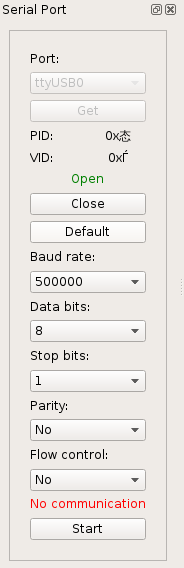
\includegraphics[width=0.2\textwidth]{images/gui/serial-port}
\caption{Serial port configuration.}
\label{fig:serial-config}
\end{figure}

\subsection{Logging and Live Plotting}

The logging software was adapted to create CSV files of all the data received from the microcontroller embedded system after it has been appropriately converted to a human readable format.

The live plotting function of the software takes an array of data of a known data size and endianness and plots the change in these values over time. There are a number of plotting options such as samples shown and format options. The live plotting proved useful for debugging of data processing issues and during experimentation to see spring-damper responses as virtual model configuration options are changed.

A number of data type conversions took place from serial reception to data plotting and logging, as follows. Qt has a number of application specific data types, usually prepended by a 'Q':

\begin{enumerate}
\item Serial data is read into the QByteArray RXBuffer.
\item RXBuffer is then copied to a char\* array to enable the packet to be decoded using the packed struct method of \cref{sec:structuring}.
\item Struct members are accessed and a union is used to convert between data types and perform calculation operations.
\item Processed data is converted to a QString using the number operator and appended to the QByteArray PlotBuffer as well as the QStringList CSVList which is converted to CSV format.
\item Finally both CSVLog and PlotBuffer are emitted as Qt signals for file logging and live plotting respectively.
\end{enumerate}

A CRC check was implemented to check the packets being received are valid. Occasionally data points are not logged or plotted - this is occasionally due to CRC failures, but usually due to the variation in processing frequency of packets due to inaccurate timing discussed in \cref{sec:Serial Communication}.

All logging and plotting development took place in the \textit{serialportwidget.cpp} file and corresponding header files and Qt forms.

The GUI for logging can be seen in \cref{fig:packet-logging} and for plotting in \cref{fig:live-plotting}.\cite{jorgeaparicio2013}

\begin{figure}
\centering
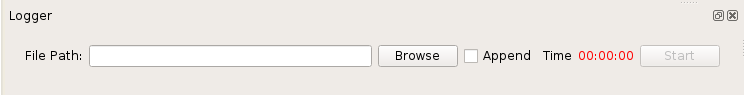
\includegraphics[width=0.5\textwidth]{images/gui/logger}
\caption{Packet data CSV logging.}
\label{fig:packet-logging}
\end{figure}

\begin{figure}
\centering
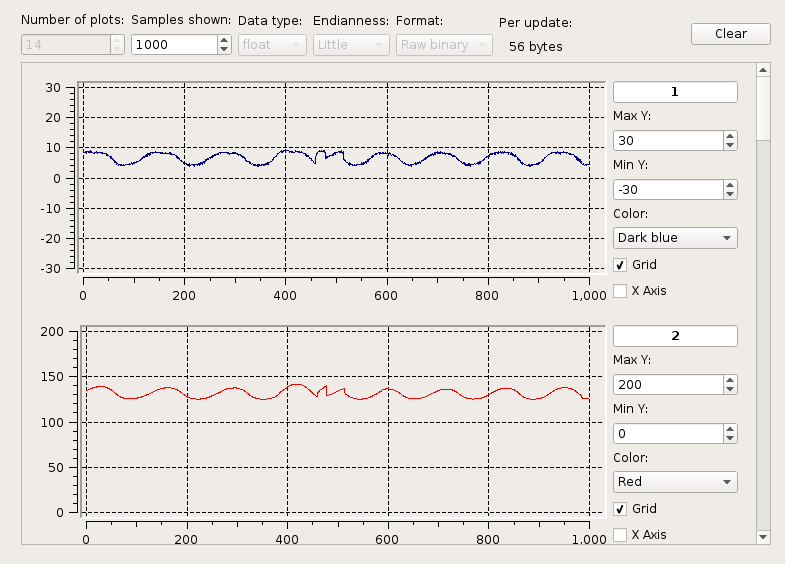
\includegraphics[width=0.5\textwidth]{images/gui/plotting}
\caption{Live plotting of motor feedback and controller data.}
\label{fig:live-plotting}
\end{figure}

\subsection{Control Plug-in}

The control plug-in was custom designed and developed for the Baleka robotic leg application. The following primary functions were integrated:

\begin{enumerate}
\item Safety.
\item Configuration.
\item Initialisation.
\item Virtual model control.
\item Sequence triggering.
\item Current and position control.
\item Control loop gain adjustment.
\end{enumerate}

The safety function of the plug-in covers not only controls to disable the motors in a case of malfunction, but also ensures that users can not enter invalid values or values that result in kinematic collisions.

The configuration and initialisation section seen in \cref{fig:Control interface plug-in} allows the motor drivers to be enabled, on-board configuration set up to be selected and the motor driver encoder position to be calibrated. 

The encoder calibration takes the current leg position and sets both $\phi_1$ and $\phi_2$ to $180^o$, measured from vertical as seen in \cref{sec:Geometry}.

The \textit{launch sequence} button combines all configuration options for a quick set up of the leg for virtual compliance or jump sequence control.

For the \textit{on-board control} and \textit{current \& position control} sections various selection boxes and text boxes exist. The underlying software ensures that, for example, current and position can not be controlled at the same time. Whenever a value changes, an update event is triggered and the data is compiled, along with an op-code, before being sent to the embedded system. The op-code then indicates to the embedded system how the data should be processed and what configuration settings should be changed.

The data processing of the control plug-in works with op-codes being added to a processing queue. When a button is pressed or a value changed, the queue is processed until empty while a switch statement based on the op-code determines where the data is placed in the packet and how it is processed. The event handlers complete the in application configuration changes.

All control plug-in functionality development took place in the \textit{framewidget.cpp} file and corresponding header files and Qt forms.

\begin{figure}
\centering
\subfloat[][Configuration \& On-board Control]{
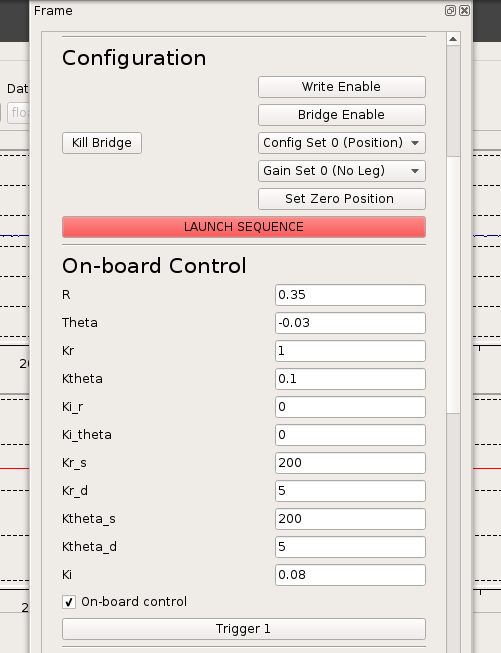
\includegraphics[width=0.4\textwidth]{images/gui/frame-1}
}
~
\subfloat[][Current/Position Control \& Control Loop Gains]{
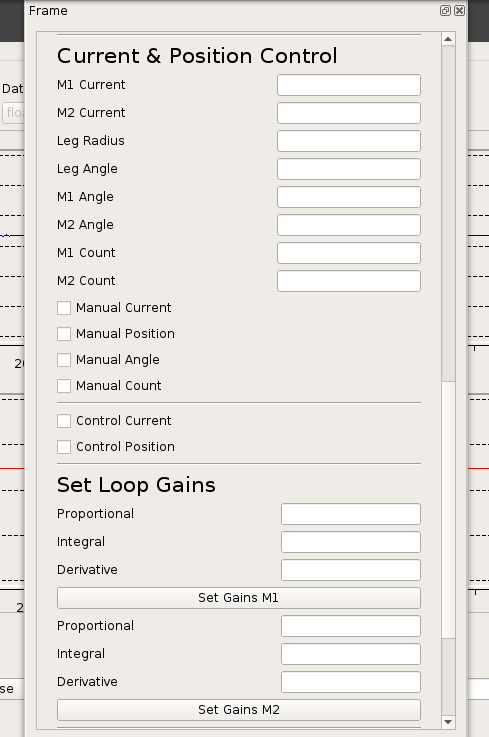
\includegraphics[width=0.4\textwidth]{images/gui/frame-2}
}
\caption{Control interface plug-in.}
\label{fig:Control interface plug-in} 
\end{figure}
\setchapterpreamble[uc][.75\textwidth]{%
\dictum[Van Halen, \textit{1984}]{%
``Jump!''}\vskip1em}
\chapter{Controller Development}

\section{Dynamic Actuation}

\setchapterpreamble[uc][.75\textwidth]{%
\dictum[Sherlock Holmes in Arthur Conan Doyle, \textit{The Adventure of the Copper Beeches}]{%
```Data! Data! Data!' he cried impatiently. `I can't make bricks without clay.'''}\vskip1em}
\chapter{Experimental Testing}

$r_0 = 0.3\ m$\\
$r_{offset} = r - r_0 = 0.13\ m$

\begin{figure}
\centering
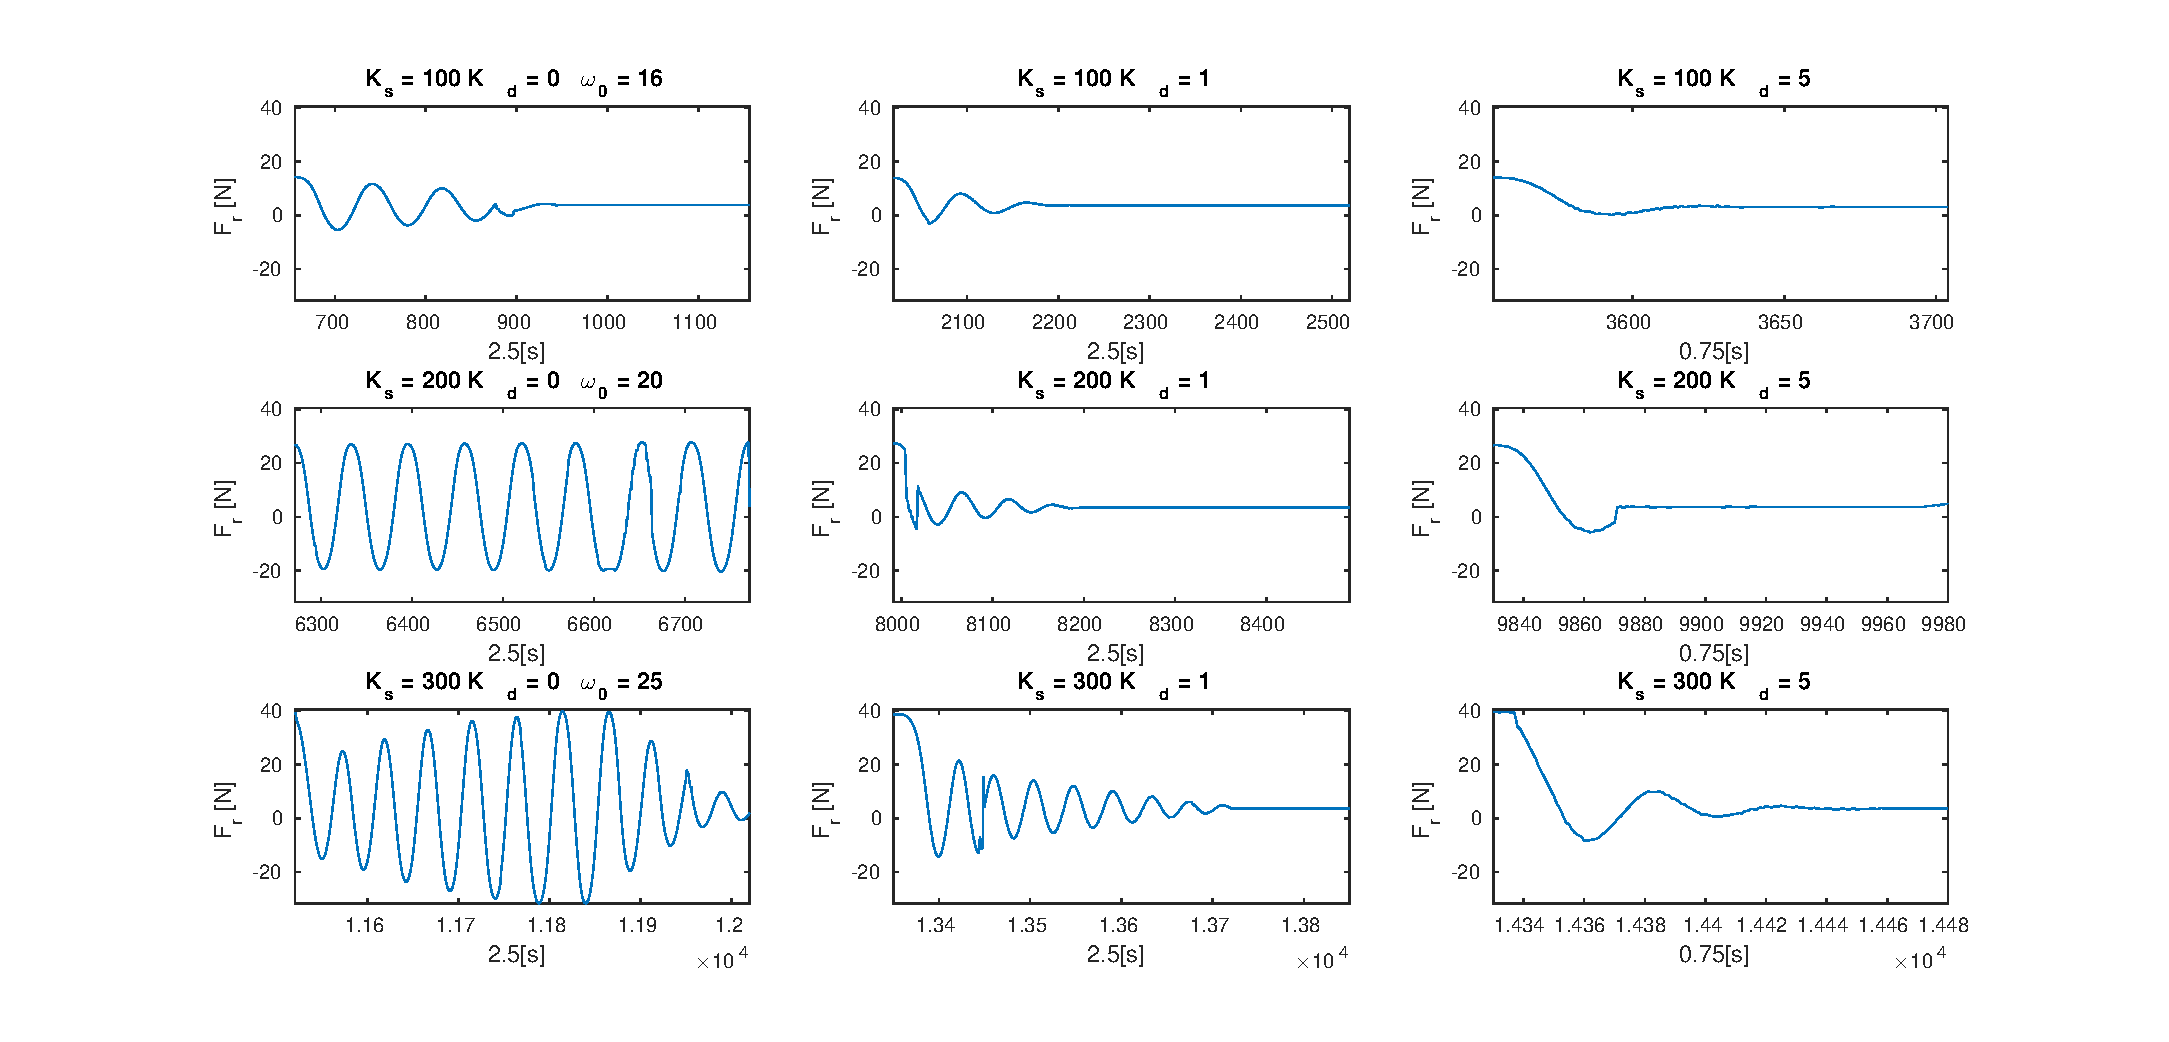
\includegraphics[width=1\textwidth]{images/logging/spring-damper-tests.eps} 
\caption{Leg spring damper testing for radial offset.}
\label{fig:spring-damper-tests}
\end{figure}
\chapter{Discussion}
\section{Design Validation}

\subsection{Robotic Testing Rig}

The testing rig, when properly lubricated to reduce mechanical impedance, performed well. The design choice to use a linear guide, instead of steel rods and ball bearings, paid off in the end - both a reduction in weight and complexity were achieved. The rig had a limited height for jump experimentation - due to the limitation in peak motor current which effectively limited the jump height to just under $0.4\ m$ the rig height was adequate. 

The testing rig enabled a number of experiments to be performed successfully including both static and dynamic tests.

\subsection{Embedded System \& GUI Design}

The embedded system design proved to be the majority of the work involved in the project. The choice of using a real time operating system to implement the communication and control enabled a complex, yes structured and easily adaptable system. The framework designed can definitely serve as a reference for future robotic projects where similar tasks are involved. 

By choosing a functional GUI, qSerialTerm, as a starting point, extensive GUI development was made possible in the short duration available. The control and command plug-ins developed, based on the same packet packing method developed during the embedded system design, are intuitive and adaptable. As further experiments were performed, Qt GUI components could be appended and integrated quickly. The cross compilation of the GUI possible for both Windows and Linux means the platform can be used for future research without concern for compatibility.

The embedded system was theoretically capable of sample rates up to approximately $800\ Hz$ with the packet sizes involved, due to limitation of the motor drivers this was not possible. The sampling rate is especially critical for virtual model applications where the response of the system needs to be consistently controlled to achieve a high fidelity response.

\section{Results Validation}

The process of modelling, simulation, implementation, and testing produced theoretical, simulated, and practical results. Using critical analysis and comparison we can validate these results. 

\subsection{Motor Current Predications}
The active compliance motor current simulation in \cref{fig:motor-current-requirements} was used to validate the motor driver peak current specification. 

The control simulation plots in \cref{fig:Control system simulation plots} showed slightly lower peak current predictions - this was expected as the control simulation was less comprehensive, whereas the active compliance motor current simulation covered all theoretical kinematic set-points. 

In reality during experimentation, as seen in \cref{fig:jump-motor-current-feedback}, the current saturated during launch, but during the other phases of jumping the current requirements predicated were correct. This was expected as the current predictions did not take into account the impulsive force needed for launching.

\Cref{fig:Current control tracking} shows the motor driver and current controller, both on-board the motor drivers and with the communication to the embedded system performed well. The minimum possible latency between current feedback and current command was achieved given the limitation of the motor driver communication system.

\subsection{Motor Torque Predications}

Motor torque predictions were performed in \cref{sec:Motor Torque Predictions}. They showed a maximum torque of approximately $4-10\ Nm$ per motor depending on the virtual model topology used. When the arc-length rotational measure was used a maximum torque of $4\ Nm$ was predicted. In practise, during the jump tests, a maximum motor torque of $4.4\ Nm$ was seen. This is not considering the motor current and torque saturation needed for launching. This validates the torque predictions simulated before testing was performed. 

\subsection{Virtual Model Fidelity}

The leg was modelled as a spring-damper system. In \cref{sec:Virtual Spring-damper Tests} this virtual model was tested to determine, amongst other aims, the fidelity of the virtual model control system. 

Various topologies were tested, and the results summarized in the analysis that followed. Although the tests showed that the natural frequency of the various responses were accurate when compared to theory, the damping factor was not easily measured for comparison - this was partially due to the use of a backwards difference velocity estimation method prior to changing to a Jacobian mapping for all further tests.

\subsection{Force Control Fidelity}

As performed in \cref{sec:Consecutive Jump Repeatability}, the experiment found that during repeated jumping, the force control system was both robust to disturbances and implemented reliable and repeatable force control.

The experiment performed in \cref{sec:Force Control Calibration and Fidelity} added to the validation of force control fidelity by showing the mechanical transparency between the motor torque and foot force coupling. In theory a linear force relationship was expected using a spring-damper model and the linear motor torque current relationship, with a varying radial offset - this was confirmed during experimentation.

Both of the above experiments show the fidelity of the force control. Although a Simulink force control simulation was performed, it was not directly comparable to the experiments, despite proving useful in determining the reliability of operation of the control system.

\section{Performance Validation}

Performance validation aims to both validate the performance of the system as originally expected during the research investigation stage, and as compared to other similar legged robots.

By considering the original problems to be investigated the following discussion can be had about the overall performance of the system:

\subsection{Problems to be Investigated}
\begin{itemize}
\item \textbf{High speed embedded system communication and packet processing:} Using a RTOS and DMA framework, high speed communication up to $800\ Hz$ was reliably achieved on the embedded system. Due to motor driver constraints this was limited to $200\ Hz$.
\item \textbf{Virtual model control for accurate end effector force output:} Virtual model control force fidelity was shown by comparing simulation and testing to theory. It was found to be accurate for the majority of the testing, but without a proper load cell system it is difficult to properly measure performance.
\item \textbf{Effective high speed kinematic control:} The kinematic control was most effectively tested during the trajectory tracking tests in \cref{sec:Trajectory Tracking}. Although accurate trajectory tracking was achieved, the high speed capabilities of the system were not extensively tested. During jump tests the maximum speed of $3\ m/s$ was tested and kinematic performance was adequate for that case.
\item \textbf{Effective use of motor drivers to achieve rapid accelerations with a direct drive BLDC motor:} The motor drivers were limited in both current peak and communication speed specifications. They performed adequately for the jump tests, but during more rapid three dimensional tests with more robotic mass or jump height needed, better motor drivers would be required.
\item \textbf{Development of a platform suitable for further use in dynamic legged motion research:} The software design is highly adaptable and capable of performing further research. The hardware design is adequate for the single vertical axis tests performed in this study, but would need to be more robust for further extensive testing.
\end{itemize}

\subsection{State of the Art Comparison}

\Cref{tbl:Robot performance comparison} provides a performance comparison of various legged robots, as compiled by \cite{Kalouche2016}.

A few of the robots that specifically use the same linkage leg design as Baleka will be compared in more depth. Although the kinematic equations derived in \cite{Duperret} were adapted for Baleka, the study did not include the necessary detail needed to compare it's performance. The GOAT leg \cite{Kalouche2016}, the ATRIAS robot \cite{jgrimes2013}, and the Minitaur robot \cite{Kenneally2016} will be critically compared.

The robots mentioned are all of different size and configurations. The GOAT leg was tested in the single leg case and the ATRIAS robot was a fully sized $60\ kg$ beast. A fair comparison between these robots would be to use the energy to mass ratio in $[J/kg]$. This ensures the energy delivered is normalized, and that the large robots don't have an unfair advantage with larger actuators.

Baleka weighed in at an energy to mass ratio of $3.9\ J/kg$, ATRIAS at $1.1\ J/kg$, GOAT at $8.0\ J/kg$, and Minitaur at $4.7\ J/kg$. The places GOAT ahead of the pack with Minitaur and Baleka following just behind. 

If on the other hand you consider the actuator mass ratio, it tells a different story. Baleka weighs in at $8.7\ J/kg$, ATRIAS at $10\ J/kg$, Minitaur at $11.75\ J/kg$, and GOAT at $16.7\ J/kg$. This means that the GOAT robot managed to get the most efficient use out of its motors, or the most energy delivered per kg of actuator. This performance measure also shows how Baleka failed to deliver as much energy due to the limitation of the motor drivers, as both the GOAT leg and Baleka leg used the same motors and virtual model control.

Considering the constraints on Baleka, it performed well for its class, delivering a middle of the range $3.9\ J/kg$. A number of the other robotic platforms did not meet these specifications, but it should also be considered that Baleka was specifically built for jumping whereas some of the robots could perform complex manoeuvres. 

Considering that Baleka was built for jumping, we should compare jump heights. Baleka achieved a maximum height of $0.4\ m$, ATRIAS $0.11\ m$, Minitaur $0.48\ m$ and GOAT $0.82\ m$. These tests are a bit more difficult to compare given the different leg topologies used. Baleka was certainly capable of performing a much higher jump given more current, but considering that the GOAT leg jumped $0.82\ m$ with approximately the same current shows that the leg design and efficiency were superior to that of Baleka, and given more time and resources should be strived for.

\begin{figure}
\centering
\subfloat[][ATRIAS.]{
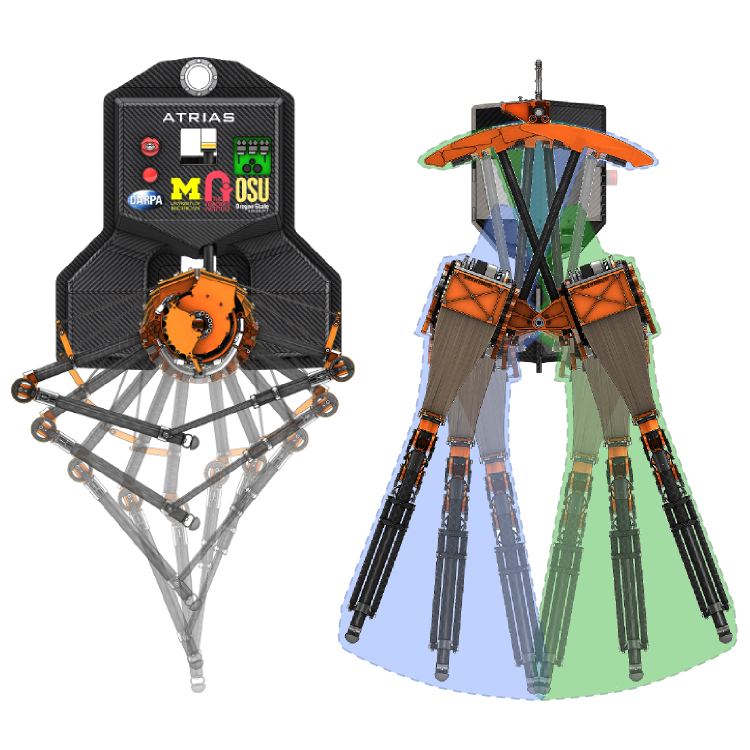
\includegraphics[width=0.3\textwidth]{images/discussion/ATRIAS.png} 
\label{fig:ATRIAS}
}
~
\subfloat[][Minitaur.]{
\includegraphics[width=0.3\textwidth]{images/discussion/Minitaur.jpeg} 
\label{fig:Minitaur}
}

\subfloat[][GOAT.]{
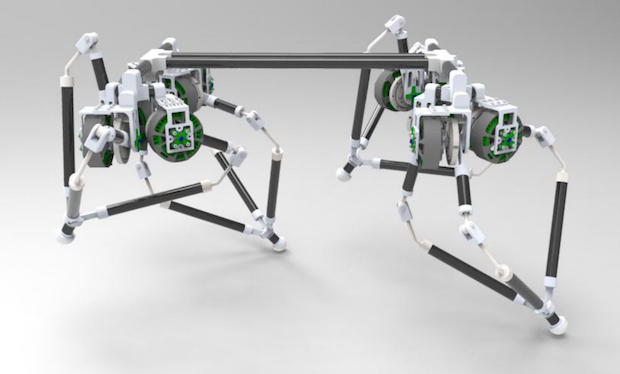
\includegraphics[width=0.3\textwidth]{images/discussion/GOAT.jpeg} 
\label{fig:GOAT}
}
\caption{Robots for performance comparison.}
\label{fig:Robots for performance comparison}
\end{figure}

\begin{table}[]
\centering
\begin{tabular}{lllllllll}
\textbf{Robot} & \textbf{\pbox{20cm}{Legs\\{[}no.{]}}} & \textbf{DoF} & \textbf{\pbox{20cm}{Leg\\Length\\{[}m{]}}} & \textbf{\pbox{20cm}{Mass\\{[}kg{]}}} & \textbf{\pbox{20cm}{Motor\\Mass\\{[}\%{]}}} & \textbf{\pbox{20cm}{Gear\\Ratio}} & \textbf{\pbox{20cm}{Jump\\Height\\{[}m{]}}} & \textbf{\pbox{20cm}{Energy\\Delivered\\{[}J{]}}} \\
\rowcolor[HTML]{67FD9A} 
Baleka         & 1                       & 2            & 0.3                         & 2.2                    & 45                           & n/a                 & 0.4                          & 8.63                              \\
Goat           & 1                       & 3            & 0.26                        & 2.5                    & 48                           & n/a                 & 0.82                         & 20.11                             \\
MIT Cheetah    & 4                       & 3            & 0.275                       & 33                     & 24                           & 5.8                 & 0.5                          & 161.9                             \\
Minitaur       & 4                       & 2            & 0.2                         & 2                      & 40                           & n/a                 & 0.48                         & 9.41                              \\
XRL            & 6                       & 1            & 0.2                         & 8                      & 11                           & 23                  & 0.425                        & 33.3                              \\
Delta Hopper   & 1                       & 3            & 0.2                         & 2                      & 38                           & n/a                 & 0.35                         & 6.9                               \\
StarlETH       & 4                       & 3            & 0.2                         & 23                     & 16                           & 100                 & 0.32                         & 72.2                              \\
HRP3La-JSK     & 2                       & 6            & 0.6                         & 54                     & 9.2                          & ??                  & 0.27                         & 143                               \\
ATRIAS         & 2                       & 3            & 0.42                        & 60                     & 11                           & 50                  & 0.11                         & 64.7                             
\end{tabular}
\caption{Legged robot performance comparison.\cite{Kalouche2016}}
\label{tbl:Robot performance comparison}
\end{table}
\setchapterpreamble[uc][.75\textwidth]{%
\dictum[C.S. Lewis, \textit{The Last Battle}]{%
``One always feels better when one has made up one's mind.''}\vskip1em}
\chapter{Conclusions}
\chapter{Recommendations and Future Work}
\lipsum
\bibliographystyle{ieeetran}
\renewcommand{\bibname}{References}
\bibliography{aux/bibliography}

\appendix
\chapter{Workspace Data}

Research data is separated into the folders as listed below, available on CD or by request:

\begin{itemize}
\item background: various literature review documents.
\item baleka-stm32f4-code: embedded system code.
\item BalekaQtApp: Qt GUI code.
\item baleka-system-kicad: start of electronics CAD representation of embedded system.
\item communication: embedded system and motor driver communication protocol work.
\item datasheets: various datasheets of components used in leg design.
\item documentation: start of documentation write-up for Driveware use and configuration.
\item drawio: draw.io graphic design application files used for report.
\item experiments: experimental test data and video data.
\item kinematics: various files with kinematic constraints and motor driver position limits.
\item LATEX: report write-up in LATEX.
\item miscellaneous: mass logs, motor model tuning, and performance tables.
\item solidworks-original: compressed folder of all Ben Bingham's original CAD work.
\item VacWorkLeg-original: compressed folder of all Luke Bell's original work.
\item workspace-atollic: initial development of embedded system code.
\item workspace-driveware: Driveware motor driver configuration files.
\item workspace-inemo: work completed on iNemo code developed by Callen Fisher.
\item workspace-matlab: Matlab scripts and saved workspaces.
\item workspace-openscad: OpenSCAD programmatic CAD models.
\item workspace-solidworks: CAD assemblies, designs and virtual models developed in Solidworks.
\end{itemize}

The final report write-up PDF can be found in the root directory, named report.pdf.
\chapter{Code}
\lipsum
\chapter{Motor Driver Command Protocol}
\label{chap:Motor Driver Command Protocol}

\begin{sidewaystable}[]
\centering
\begin{tabular}{llllllll}
\textbf{Command}  & \textbf{\pbox{20cm}{Packet\\Index}} & \textbf{\pbox{20cm}{Command\\Bits}} & \textbf{\pbox{20cm}{Sequence Bits\\ (Op-code)}} & \textbf{\pbox{20cm}{Address\\Index}} & \textbf{\pbox{20cm}{Address\\Offset}} & \textbf{Function}                    & \textbf{Notes}         \\
KILL\_BRIDGE       & 0                     & 0x02                  & 0001                             & 0x01                   & 0x00                    & \pbox{20cm}{Kill motor\\ driver bridge.}            &                        \\
WRITE\_ENABLE      & 1                     & 0x02                  & 0010                             & 0x07                   & 0x00                    & Enable write access.                 &                        \\
BRIDGE\_ENABLE     & 2                     & 0x02                  & 0100                             & 0x01                   & 0x00                    & \pbox{20cm}{Enable motor\\ driver bridge.}          &                        \\
CURRENT\_COMMAND   & 20/21                 & 0x02                  & 0011                             & 0x45                   & 0x02                    & Command a current.                   & Conversion needed.     \\
POSITION\_COMMAND  & 22/23                 & 0x02                  & 1010                             & 0x45                   & 0x00                    & Command a position                   & Conversion needed.     \\
READ\_CURRENT      & 5                     & 0x01                  & 1100                             & 0x10                   & 0x03                    & Read current motor.                  & Conversion needed.     \\
READ\_POSITION     & 6                     & 0x01                  & 1111                             & 0x12                   & 0x00                    & \pbox{20cm}{Read motor position\\ in counts.}       & Conversion needed.     \\
READ\_VELOCITY     & 7                     & 0x01                  & 0101                             & 0x11                   & 0x02                    & \pbox{20cm}{Read motor velocity\\ in cts/s.}        & Conversion needed.     \\
ZERO\_POSITION     & 8                     & 0x02                  &                                  & 0x01                   & 0x00                    & \pbox{20cm}{Re-callibrate encoder\\ zero position.} &                        \\
GAIN\_SET          & 9                     & 0x02                  &                                  & 0x01                   & 0x01                    & \pbox{20cm}{Select gain set\\ 1 or 2.}              & Requires bit toggling. \\
GAIN\_CHANGE\_M1: P & 10                    & 0x02                  &                                  & 0x38                   & 0x00                    & \pbox{20cm}{Set driver position\\ loop gain.}       &                        \\
GAIN\_CHANGE\_M1: I & 11                    & 0x02                  &                                  & 0x38                   & 0x02                    & \pbox{20cm}{Set driver position\\ loop gain.}       &                        \\
GAIN\_CHANGE\_M1: D & 12                    & 0x02                  &                                  & 0x38                   & 0x04                    & \pbox{20cm}{Set driver position\\ loop gain.}       &                        \\
GAIN\_CHANGE\_M2: P & 13                    & 0x02                  &                                  & 0x38                   & 0x00                    & \pbox{20cm}{Set driver position\\ loop gain.}       &                        \\
GAIN\_CHANGE\_M2: I & 14                    & 0x02                  &                                  & 0x38                   & 0x02                    & \pbox{20cm}{Set driver position\\ loop gain.}       &                        \\
GAIN\_CHANGE\_M2: D & 15                    & 0x02                  &                                  & 0x38                   & 0x04                    & \pbox{20cm}{Set driver position\\ loop gain.}       &                        \\
CONFIG\_SET        & 16                    & 0x02                  & 1001                             & 0xD1                   & 0x00                    & \pbox{20cm}{Select configuration\\ 1 or 2.}         & Requires bit toggling.
\end{tabular}
\caption{Motor driver command protocol.}
\label{tbl:motor-driver-protocol}
\end{sidewaystable}
\chapter{Geometric Simulation Code}

\begin{listing}[ht]
\begin{minted}[
linenos,
bgcolor=smokyblack]{Matlab}
l1 = 0.15; %length of upper linkage in m (measured from center of joint of 5 cm diameter)
l2 = 0.3; %length of lower linkage in m (measured from center of joint of 5 cm diameter)

phi1 = (1/9*pi):0.125:pi; % all possible phi1 values
phi2 = (1/9*pi):0.125:pi; % all possible phi2 values

[PHI1, PHI2] = meshgrid(phi1, phi2); % generate a grid of phi1 and phi2 values

R = -l1*cos((PHI1 + PHI2)./2) + sqrt(l2^2 - l1^2*sin((PHI1 + PHI2)./2).^2);
THETA = (PHI1 - PHI2)./2;

plot(THETA(:), R(:), 'r.', 'MarkerSize', 20);
\end{minted}
\caption{Geometric simulation code to generate kinematic workspace.}
\label{listing:Geometric simulation code}
\end{listing}
\chapter{Jump Experiment}
\label{app:Jump Experiment}

\begin{table}[!ht]
\centering
\begin{tabular}{l|llll}
\textbf{Frame (no.)} & \textbf{Time (ms)} & \textbf{Height (m)} & \textbf{Interval Velocity (m/s)} & \textbf{Phase}\\
0	&	0	&	0.00000	&	0.000	&	Stance	\\
1	&	84	&	0.05000	&	0.595	&	Decompression launch	\\
2	&	126	&	0.12500	&	1.786	&	Decompression launch	\\
3	&	167	&	0.21250	&	2.134	&	Flight	\\	
4	&	209	&	0.25000	&	0.893	&	Flight + Recovery	\\
5	&	292	&	0.29375	&	0.527	&	Flight + Recovery	\\
6	&	376	&	0.26250	&	-0.372	&	Freefall	\\
7	&	501	&	0.12500	&	-1.100	&	Freefall	\\
8	&	543	&	0.07500	&	-1.190	&	Impact	\\
9	&	584	&	0.00000	&	-1.829	&	Compliant landing	\\
10	&	709	&	0.02500	&	0.200	&	Compliant landing	\\
11	&	793	&	0.04375	&	0.223	&	Compliant landing
\end{tabular}
\caption{Launch and compliant landing video frame data.}
\label{tab:jump-test-data}
\end{table}

\begin{figure}
\centering
\subfloat[][Frame 0.]{
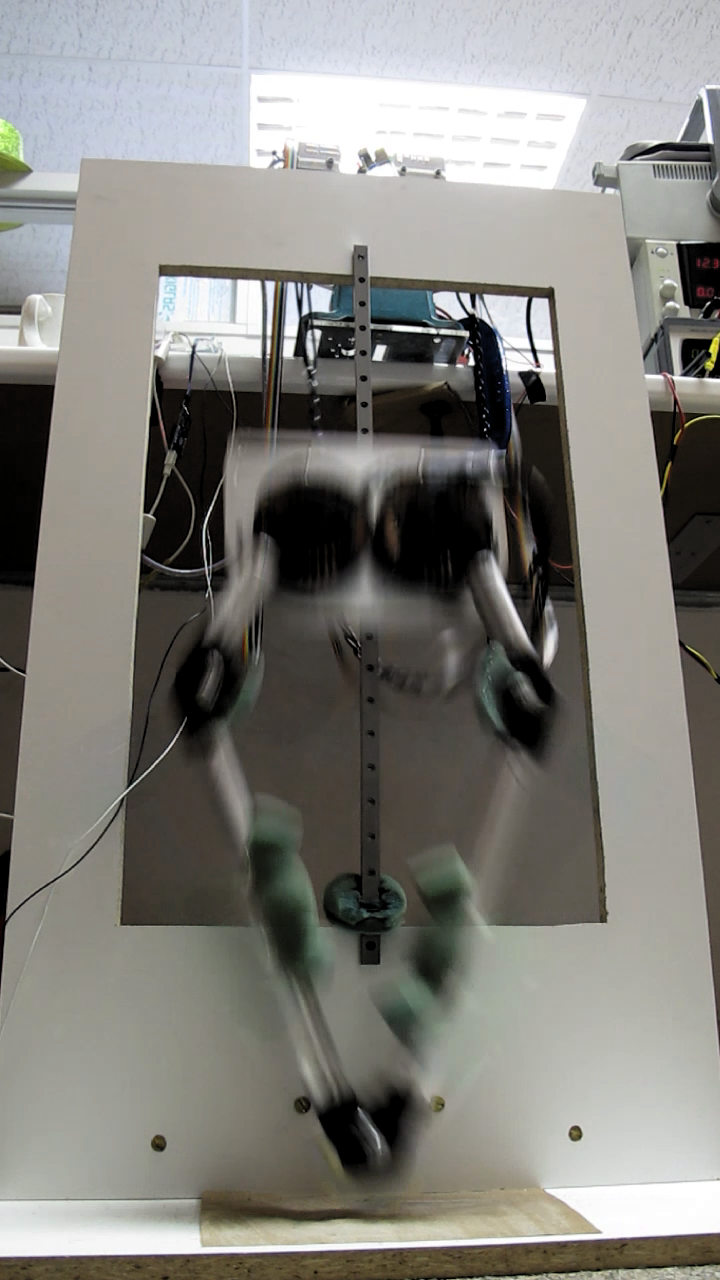
\includegraphics[width=0.3\textwidth]{images/experiments/failed-jump/0.png} 
}
~
\subfloat[][Frame 1: Current cut-out.]{
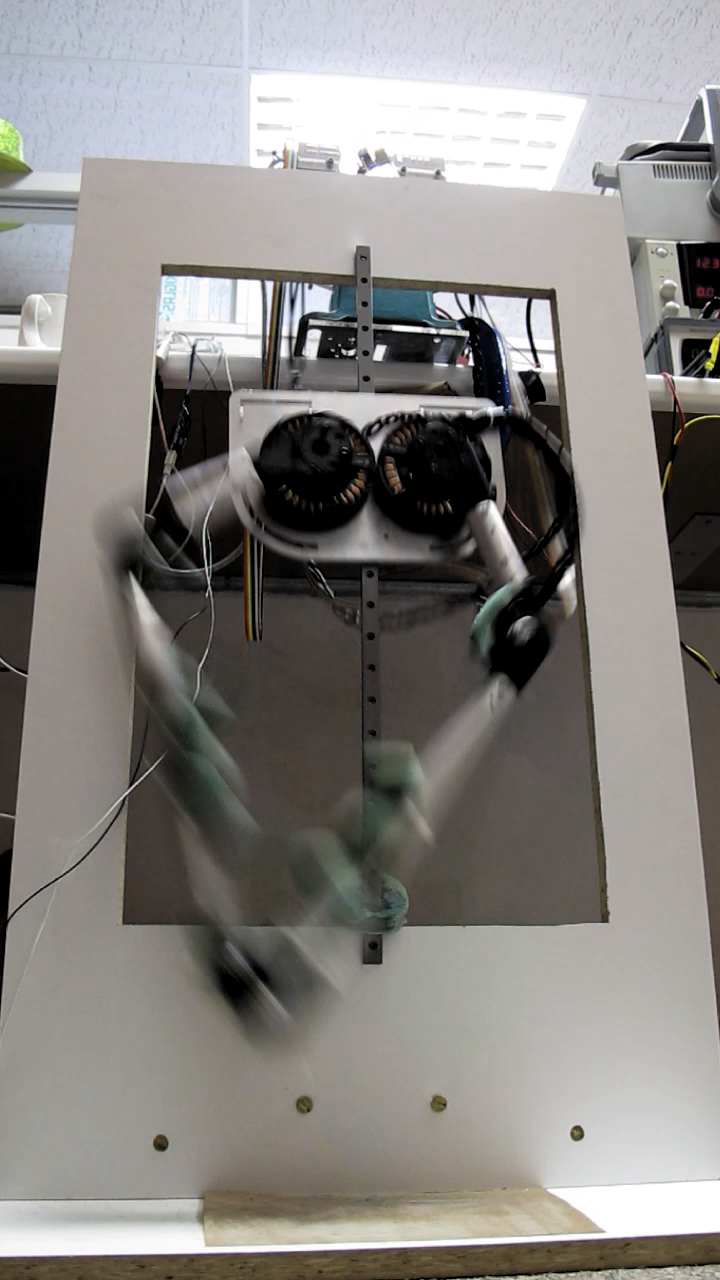
\includegraphics[width=0.3\textwidth]{images/experiments/failed-jump/1.png} 
}
~
\subfloat[][Frame 2.]{
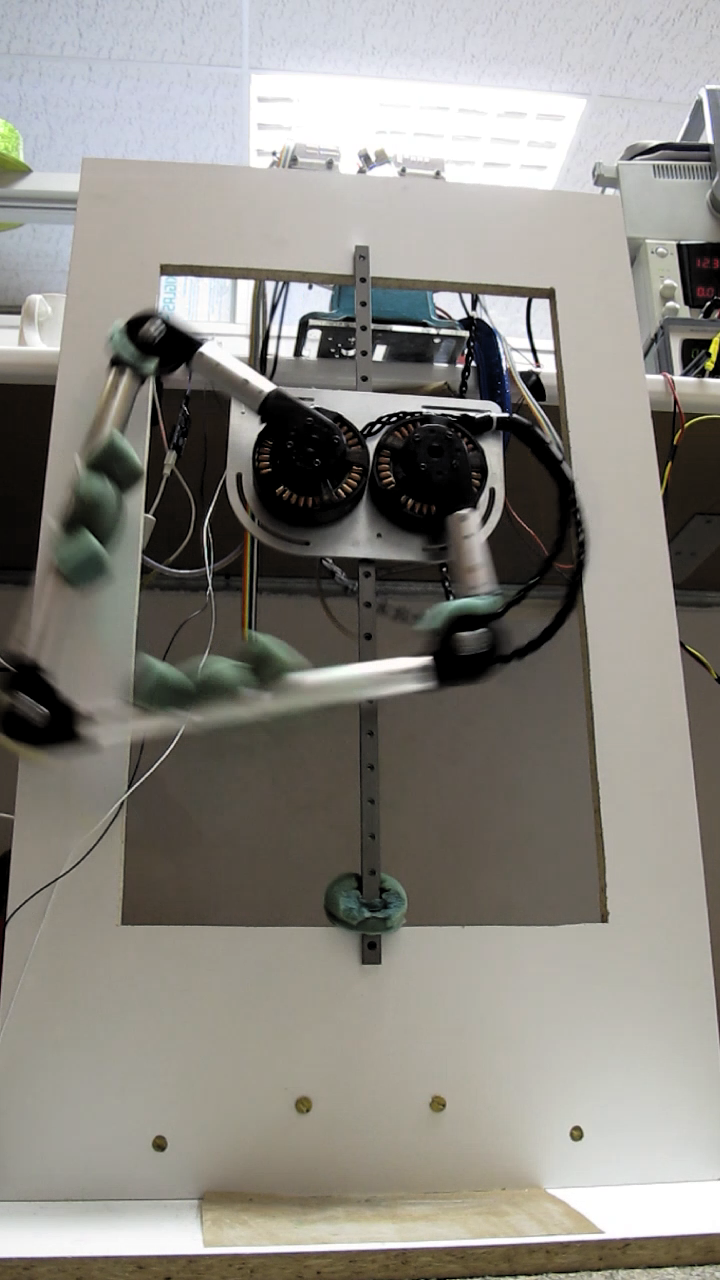
\includegraphics[width=0.3\textwidth]{images/experiments/failed-jump/2.png} 
}

\subfloat[][Frame 3.]{
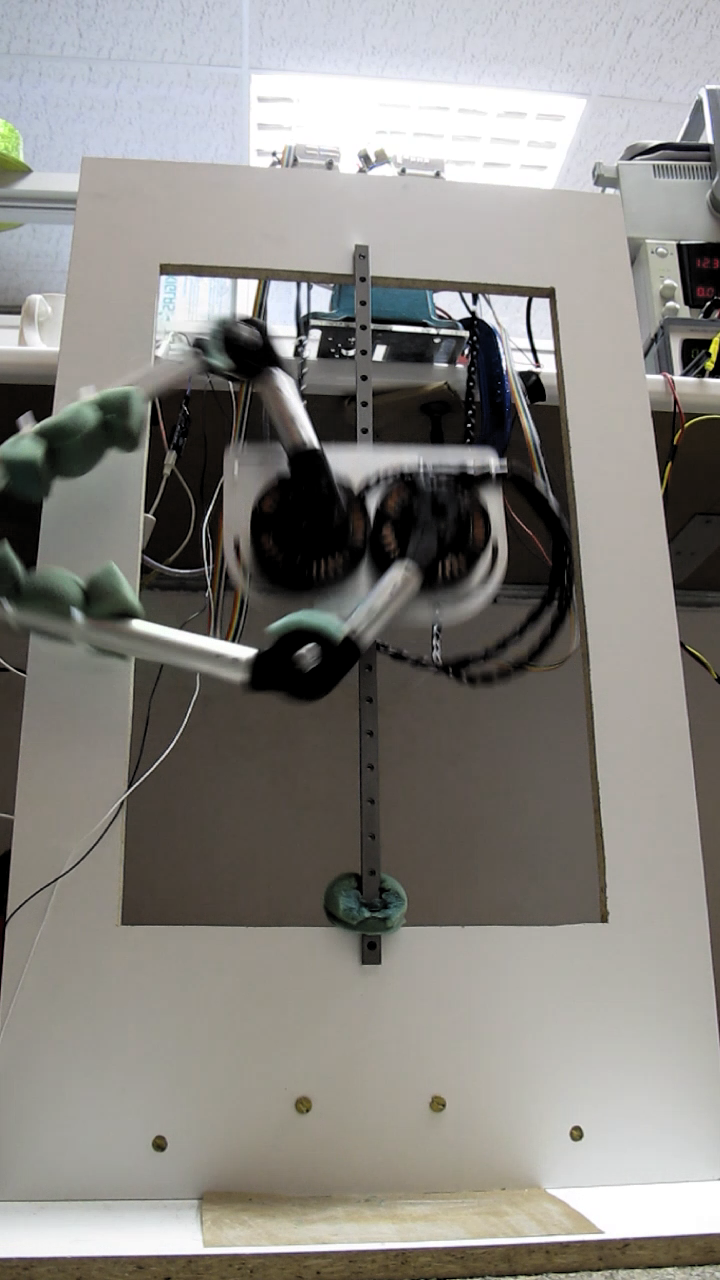
\includegraphics[width=0.3\textwidth]{images/experiments/failed-jump/3.png} 
}
~
\subfloat[][Frame 4.]{
\includegraphics[width=0.3\textwidth]{images/experiments/failed-jump/4.png} 
}
~
\subfloat[][Frame 5.]{
\includegraphics[width=0.3\textwidth]{images/experiments/failed-jump/5.png} 
}
\caption{Motor driver over-current cut-out.}
\label{fig:Motor driver over-current cut-out}
\end{figure}

\begin{listing}[ht]
\begin{minted}[
linenos,
bgcolor=smokyblack]{c}
if(SHOT && r_fbk >= 0.38) {
        r_cmd = 0.3;
        k_r = 1;
        k_s = 0.1;
        ks_r = 633;
        kd_r = 15;
        ks_s = 400;
        kd_s = 5;
        SHOT = 0;
        TRIGGER = 1; //DANGEROUS!
}
if(PULLED && (ELAPSED > 1000)) {
        r_cmd = 0.4;
        k_r = 1;
        k_s = 0.1;
        ks_r = 1726;
        kd_r = 0;
        ks_s = 400;
        kd_s = 5;
        SHOT = 1;
        PULLED = 0;
        ELAPSED = 0;
}
if(TRIGGER) {
        r_cmd = 0.25;
        k_r = 1;
        k_s = 0.1;
        ks_r = 633;
        kd_r = 15;
        ks_s = 400;
        kd_s = 5;
        ELAPSED = 0;
        TRIGGER = 0;
        PULLED = 1;
}
else{
        ELAPSED++;
}
\end{minted}
\caption{Jump control condition loop.}
\label{listing:Jump control condition loop}
\end{listing}

\end{document}
